% Options for packages loaded elsewhere
\PassOptionsToPackage{unicode}{hyperref}
\PassOptionsToPackage{hyphens}{url}
%
\documentclass[
]{article}
\usepackage{lmodern}
\usepackage{amssymb,amsmath}
\usepackage{ifxetex,ifluatex}
\ifnum 0\ifxetex 1\fi\ifluatex 1\fi=0 % if pdftex
  \usepackage[T1]{fontenc}
  \usepackage[utf8]{inputenc}
  \usepackage{textcomp} % provide euro and other symbols
\else % if luatex or xetex
  \usepackage{unicode-math}
  \defaultfontfeatures{Scale=MatchLowercase}
  \defaultfontfeatures[\rmfamily]{Ligatures=TeX,Scale=1}
\fi
% Use upquote if available, for straight quotes in verbatim environments
\IfFileExists{upquote.sty}{\usepackage{upquote}}{}
\IfFileExists{microtype.sty}{% use microtype if available
  \usepackage[]{microtype}
  \UseMicrotypeSet[protrusion]{basicmath} % disable protrusion for tt fonts
}{}
\makeatletter
\@ifundefined{KOMAClassName}{% if non-KOMA class
  \IfFileExists{parskip.sty}{%
    \usepackage{parskip}
  }{% else
    \setlength{\parindent}{0pt}
    \setlength{\parskip}{6pt plus 2pt minus 1pt}}
}{% if KOMA class
  \KOMAoptions{parskip=half}}
\makeatother
\usepackage{xcolor}
\IfFileExists{xurl.sty}{\usepackage{xurl}}{} % add URL line breaks if available
\IfFileExists{bookmark.sty}{\usepackage{bookmark}}{\usepackage{hyperref}}
\hypersetup{
  pdftitle={Codebook for tidydatasub},
  hidelinks,
  pdfcreator={LaTeX via pandoc}}
\urlstyle{same} % disable monospaced font for URLs
\usepackage[margin=2cm]{geometry}
\usepackage{longtable,booktabs}
% Correct order of tables after \paragraph or \subparagraph
\usepackage{etoolbox}
\makeatletter
\patchcmd\longtable{\par}{\if@noskipsec\mbox{}\fi\par}{}{}
\makeatother
% Allow footnotes in longtable head/foot
\IfFileExists{footnotehyper.sty}{\usepackage{footnotehyper}}{\usepackage{footnote}}
\makesavenoteenv{longtable}
\usepackage{graphicx,grffile}
\makeatletter
\def\maxwidth{\ifdim\Gin@nat@width>\linewidth\linewidth\else\Gin@nat@width\fi}
\def\maxheight{\ifdim\Gin@nat@height>\textheight\textheight\else\Gin@nat@height\fi}
\makeatother
% Scale images if necessary, so that they will not overflow the page
% margins by default, and it is still possible to overwrite the defaults
% using explicit options in \includegraphics[width, height, ...]{}
\setkeys{Gin}{width=\maxwidth,height=\maxheight,keepaspectratio}
% Set default figure placement to htbp
\makeatletter
\def\fps@figure{htbp}
\makeatother
\setlength{\emergencystretch}{3em} % prevent overfull lines
\providecommand{\tightlist}{%
  \setlength{\itemsep}{0pt}\setlength{\parskip}{0pt}}
\setcounter{secnumdepth}{-\maxdimen} % remove section numbering
\newcommand{\fullline}{\noindent\makebox[\linewidth]{\rule{\textwidth}{0.4pt}}}
\renewcommand\familydefault{\sfdefault}
\newcommand{\bminione}{\begin{minipage}{0.75 \textwidth}}
\newcommand{\bminitwo}{\begin{minipage}{0.25 \textwidth}}
\newcommand{\emini}{\end{minipage}}

\title{Codebook for tidydatasub}
\usepackage{etoolbox}
\makeatletter
\providecommand{\subtitle}[1]{% add subtitle to \maketitle
  \apptocmd{\@title}{\par {\large #1 \par}}{}{}
}
\makeatother
\subtitle{Autogenerated data summary from dataMaid}
\author{}
\date{\vspace{-2.5em}2020-12-29 16:24:28}

\begin{document}
\maketitle

\hypertarget{data-report-overview}{%
\section{Data report overview}\label{data-report-overview}}

The dataset examined has the following dimensions:

\begin{longtable}[]{@{}lr@{}}
\toprule
\begin{minipage}[b]{0.33\columnwidth}\raggedright
Feature\strut
\end{minipage} & \begin{minipage}[b]{0.12\columnwidth}\raggedleft
Result\strut
\end{minipage}\tabularnewline
\midrule
\endhead
\begin{minipage}[t]{0.33\columnwidth}\raggedright
Number of observations\strut
\end{minipage} & \begin{minipage}[t]{0.12\columnwidth}\raggedleft
180\strut
\end{minipage}\tabularnewline
\begin{minipage}[t]{0.33\columnwidth}\raggedright
Number of variables\strut
\end{minipage} & \begin{minipage}[t]{0.12\columnwidth}\raggedleft
81\strut
\end{minipage}\tabularnewline
\bottomrule
\end{longtable}

\hypertarget{codebook-summary-table}{%
\section{Codebook summary table}\label{codebook-summary-table}}

\begin{longtable}[]{@{}lllrcl@{}}
\toprule
\begin{minipage}[b]{0.06\columnwidth}\raggedright
Label\strut
\end{minipage} & \begin{minipage}[b]{0.45\columnwidth}\raggedright
Variable\strut
\end{minipage} & \begin{minipage}[b]{0.08\columnwidth}\raggedright
Class\strut
\end{minipage} & \begin{minipage}[b]{0.08\columnwidth}\raggedleft
\# unique values\strut
\end{minipage} & \begin{minipage}[b]{0.07\columnwidth}\centering
Missing\strut
\end{minipage} & \begin{minipage}[b]{0.10\columnwidth}\raggedright
Description\strut
\end{minipage}\tabularnewline
\midrule
\endhead
\begin{minipage}[t]{0.06\columnwidth}\raggedright
\strut
\end{minipage} & \begin{minipage}[t]{0.45\columnwidth}\raggedright
\textbf{\protect\hyperlink{activity}{activity}}\strut
\end{minipage} & \begin{minipage}[t]{0.08\columnwidth}\raggedright
character\strut
\end{minipage} & \begin{minipage}[t]{0.08\columnwidth}\raggedleft
6\strut
\end{minipage} & \begin{minipage}[t]{0.07\columnwidth}\centering
0.00 \%\strut
\end{minipage} & \begin{minipage}[t]{0.10\columnwidth}\raggedright
\strut
\end{minipage}\tabularnewline
\begin{minipage}[t]{0.06\columnwidth}\raggedright
\strut
\end{minipage} & \begin{minipage}[t]{0.45\columnwidth}\raggedright
\textbf{\protect\hyperlink{subject}{subject}}\strut
\end{minipage} & \begin{minipage}[t]{0.08\columnwidth}\raggedright
integer\strut
\end{minipage} & \begin{minipage}[t]{0.08\columnwidth}\raggedleft
30\strut
\end{minipage} & \begin{minipage}[t]{0.07\columnwidth}\centering
0.00 \%\strut
\end{minipage} & \begin{minipage}[t]{0.10\columnwidth}\raggedright
\strut
\end{minipage}\tabularnewline
\begin{minipage}[t]{0.06\columnwidth}\raggedright
\strut
\end{minipage} & \begin{minipage}[t]{0.45\columnwidth}\raggedright
\textbf{\protect\hyperlink{timedomain_bodyacceleration_-mean--x}{Timedomain\_BodyAcceleration\_-mean
-X}}\strut
\end{minipage} & \begin{minipage}[t]{0.08\columnwidth}\raggedright
numeric\strut
\end{minipage} & \begin{minipage}[t]{0.08\columnwidth}\raggedleft
180\strut
\end{minipage} & \begin{minipage}[t]{0.07\columnwidth}\centering
0.00 \%\strut
\end{minipage} & \begin{minipage}[t]{0.10\columnwidth}\raggedright
\strut
\end{minipage}\tabularnewline
\begin{minipage}[t]{0.06\columnwidth}\raggedright
\strut
\end{minipage} & \begin{minipage}[t]{0.45\columnwidth}\raggedright
\textbf{\protect\hyperlink{timedomain_bodyacceleration_-mean--y}{Timedomain\_BodyAcceleration\_-mean
-Y}}\strut
\end{minipage} & \begin{minipage}[t]{0.08\columnwidth}\raggedright
numeric\strut
\end{minipage} & \begin{minipage}[t]{0.08\columnwidth}\raggedleft
180\strut
\end{minipage} & \begin{minipage}[t]{0.07\columnwidth}\centering
0.00 \%\strut
\end{minipage} & \begin{minipage}[t]{0.10\columnwidth}\raggedright
\strut
\end{minipage}\tabularnewline
\begin{minipage}[t]{0.06\columnwidth}\raggedright
\strut
\end{minipage} & \begin{minipage}[t]{0.45\columnwidth}\raggedright
\textbf{\protect\hyperlink{timedomain_bodyacceleration_-mean--z}{Timedomain\_BodyAcceleration\_-mean
-Z}}\strut
\end{minipage} & \begin{minipage}[t]{0.08\columnwidth}\raggedright
numeric\strut
\end{minipage} & \begin{minipage}[t]{0.08\columnwidth}\raggedleft
180\strut
\end{minipage} & \begin{minipage}[t]{0.07\columnwidth}\centering
0.00 \%\strut
\end{minipage} & \begin{minipage}[t]{0.10\columnwidth}\raggedright
\strut
\end{minipage}\tabularnewline
\begin{minipage}[t]{0.06\columnwidth}\raggedright
\strut
\end{minipage} & \begin{minipage}[t]{0.45\columnwidth}\raggedright
\textbf{\protect\hyperlink{timedomain_bodyacceleration_-standard-deviation--x}{Timedomain\_BodyAcceleration\_-Standard-Deviation
-X}}\strut
\end{minipage} & \begin{minipage}[t]{0.08\columnwidth}\raggedright
numeric\strut
\end{minipage} & \begin{minipage}[t]{0.08\columnwidth}\raggedleft
180\strut
\end{minipage} & \begin{minipage}[t]{0.07\columnwidth}\centering
0.00 \%\strut
\end{minipage} & \begin{minipage}[t]{0.10\columnwidth}\raggedright
\strut
\end{minipage}\tabularnewline
\begin{minipage}[t]{0.06\columnwidth}\raggedright
\strut
\end{minipage} & \begin{minipage}[t]{0.45\columnwidth}\raggedright
\textbf{\protect\hyperlink{timedomain_bodyacceleration_-standard-deviation--y}{Timedomain\_BodyAcceleration\_-Standard-Deviation
-Y}}\strut
\end{minipage} & \begin{minipage}[t]{0.08\columnwidth}\raggedright
numeric\strut
\end{minipage} & \begin{minipage}[t]{0.08\columnwidth}\raggedleft
180\strut
\end{minipage} & \begin{minipage}[t]{0.07\columnwidth}\centering
0.00 \%\strut
\end{minipage} & \begin{minipage}[t]{0.10\columnwidth}\raggedright
\strut
\end{minipage}\tabularnewline
\begin{minipage}[t]{0.06\columnwidth}\raggedright
\strut
\end{minipage} & \begin{minipage}[t]{0.45\columnwidth}\raggedright
\textbf{\protect\hyperlink{timedomain_bodyacceleration_-standard-deviation--z}{Timedomain\_BodyAcceleration\_-Standard-Deviation
-Z}}\strut
\end{minipage} & \begin{minipage}[t]{0.08\columnwidth}\raggedright
numeric\strut
\end{minipage} & \begin{minipage}[t]{0.08\columnwidth}\raggedleft
180\strut
\end{minipage} & \begin{minipage}[t]{0.07\columnwidth}\centering
0.00 \%\strut
\end{minipage} & \begin{minipage}[t]{0.10\columnwidth}\raggedright
\strut
\end{minipage}\tabularnewline
\begin{minipage}[t]{0.06\columnwidth}\raggedright
\strut
\end{minipage} & \begin{minipage}[t]{0.45\columnwidth}\raggedright
\textbf{\protect\hyperlink{timedomain_gravityacceleration_-mean--x}{Timedomain\_GravityAcceleration\_-mean
-X}}\strut
\end{minipage} & \begin{minipage}[t]{0.08\columnwidth}\raggedright
numeric\strut
\end{minipage} & \begin{minipage}[t]{0.08\columnwidth}\raggedleft
180\strut
\end{minipage} & \begin{minipage}[t]{0.07\columnwidth}\centering
0.00 \%\strut
\end{minipage} & \begin{minipage}[t]{0.10\columnwidth}\raggedright
\strut
\end{minipage}\tabularnewline
\begin{minipage}[t]{0.06\columnwidth}\raggedright
\strut
\end{minipage} & \begin{minipage}[t]{0.45\columnwidth}\raggedright
\textbf{\protect\hyperlink{timedomain_gravityacceleration_-mean--y}{Timedomain\_GravityAcceleration\_-mean
-Y}}\strut
\end{minipage} & \begin{minipage}[t]{0.08\columnwidth}\raggedright
numeric\strut
\end{minipage} & \begin{minipage}[t]{0.08\columnwidth}\raggedleft
180\strut
\end{minipage} & \begin{minipage}[t]{0.07\columnwidth}\centering
0.00 \%\strut
\end{minipage} & \begin{minipage}[t]{0.10\columnwidth}\raggedright
\strut
\end{minipage}\tabularnewline
\begin{minipage}[t]{0.06\columnwidth}\raggedright
\strut
\end{minipage} & \begin{minipage}[t]{0.45\columnwidth}\raggedright
\textbf{\protect\hyperlink{timedomain_gravityacceleration_-mean--z}{Timedomain\_GravityAcceleration\_-mean
-Z}}\strut
\end{minipage} & \begin{minipage}[t]{0.08\columnwidth}\raggedright
numeric\strut
\end{minipage} & \begin{minipage}[t]{0.08\columnwidth}\raggedleft
180\strut
\end{minipage} & \begin{minipage}[t]{0.07\columnwidth}\centering
0.00 \%\strut
\end{minipage} & \begin{minipage}[t]{0.10\columnwidth}\raggedright
\strut
\end{minipage}\tabularnewline
\begin{minipage}[t]{0.06\columnwidth}\raggedright
\strut
\end{minipage} & \begin{minipage}[t]{0.45\columnwidth}\raggedright
\textbf{\protect\hyperlink{timedomain_gravityacceleration_-standard-deviation--x}{Timedomain\_GravityAcceleration\_-Standard-Deviation
-X}}\strut
\end{minipage} & \begin{minipage}[t]{0.08\columnwidth}\raggedright
numeric\strut
\end{minipage} & \begin{minipage}[t]{0.08\columnwidth}\raggedleft
180\strut
\end{minipage} & \begin{minipage}[t]{0.07\columnwidth}\centering
0.00 \%\strut
\end{minipage} & \begin{minipage}[t]{0.10\columnwidth}\raggedright
\strut
\end{minipage}\tabularnewline
\begin{minipage}[t]{0.06\columnwidth}\raggedright
\strut
\end{minipage} & \begin{minipage}[t]{0.45\columnwidth}\raggedright
\textbf{\protect\hyperlink{timedomain_gravityacceleration_-standard-deviation--y}{Timedomain\_GravityAcceleration\_-Standard-Deviation
-Y}}\strut
\end{minipage} & \begin{minipage}[t]{0.08\columnwidth}\raggedright
numeric\strut
\end{minipage} & \begin{minipage}[t]{0.08\columnwidth}\raggedleft
180\strut
\end{minipage} & \begin{minipage}[t]{0.07\columnwidth}\centering
0.00 \%\strut
\end{minipage} & \begin{minipage}[t]{0.10\columnwidth}\raggedright
\strut
\end{minipage}\tabularnewline
\begin{minipage}[t]{0.06\columnwidth}\raggedright
\strut
\end{minipage} & \begin{minipage}[t]{0.45\columnwidth}\raggedright
\textbf{\protect\hyperlink{timedomain_gravityacceleration_-standard-deviation--z}{Timedomain\_GravityAcceleration\_-Standard-Deviation
-Z}}\strut
\end{minipage} & \begin{minipage}[t]{0.08\columnwidth}\raggedright
numeric\strut
\end{minipage} & \begin{minipage}[t]{0.08\columnwidth}\raggedleft
180\strut
\end{minipage} & \begin{minipage}[t]{0.07\columnwidth}\centering
0.00 \%\strut
\end{minipage} & \begin{minipage}[t]{0.10\columnwidth}\raggedright
\strut
\end{minipage}\tabularnewline
\begin{minipage}[t]{0.06\columnwidth}\raggedright
\strut
\end{minipage} & \begin{minipage}[t]{0.45\columnwidth}\raggedright
\textbf{\protect\hyperlink{timedomain_bodyacceleration_jerk-mean--x}{Timedomain\_BodyAcceleration\_Jerk-mean
-X}}\strut
\end{minipage} & \begin{minipage}[t]{0.08\columnwidth}\raggedright
numeric\strut
\end{minipage} & \begin{minipage}[t]{0.08\columnwidth}\raggedleft
180\strut
\end{minipage} & \begin{minipage}[t]{0.07\columnwidth}\centering
0.00 \%\strut
\end{minipage} & \begin{minipage}[t]{0.10\columnwidth}\raggedright
\strut
\end{minipage}\tabularnewline
\begin{minipage}[t]{0.06\columnwidth}\raggedright
\strut
\end{minipage} & \begin{minipage}[t]{0.45\columnwidth}\raggedright
\textbf{\protect\hyperlink{timedomain_bodyacceleration_jerk-mean--y}{Timedomain\_BodyAcceleration\_Jerk-mean
-Y}}\strut
\end{minipage} & \begin{minipage}[t]{0.08\columnwidth}\raggedright
numeric\strut
\end{minipage} & \begin{minipage}[t]{0.08\columnwidth}\raggedleft
180\strut
\end{minipage} & \begin{minipage}[t]{0.07\columnwidth}\centering
0.00 \%\strut
\end{minipage} & \begin{minipage}[t]{0.10\columnwidth}\raggedright
\strut
\end{minipage}\tabularnewline
\begin{minipage}[t]{0.06\columnwidth}\raggedright
\strut
\end{minipage} & \begin{minipage}[t]{0.45\columnwidth}\raggedright
\textbf{\protect\hyperlink{timedomain_bodyacceleration_jerk-mean--z}{Timedomain\_BodyAcceleration\_Jerk-mean
-Z}}\strut
\end{minipage} & \begin{minipage}[t]{0.08\columnwidth}\raggedright
numeric\strut
\end{minipage} & \begin{minipage}[t]{0.08\columnwidth}\raggedleft
180\strut
\end{minipage} & \begin{minipage}[t]{0.07\columnwidth}\centering
0.00 \%\strut
\end{minipage} & \begin{minipage}[t]{0.10\columnwidth}\raggedright
\strut
\end{minipage}\tabularnewline
\begin{minipage}[t]{0.06\columnwidth}\raggedright
\strut
\end{minipage} & \begin{minipage}[t]{0.45\columnwidth}\raggedright
\textbf{\protect\hyperlink{timedomain_bodyacceleration_jerk-standard-deviation--x}{Timedomain\_BodyAcceleration\_Jerk-Standard-Deviation
-X}}\strut
\end{minipage} & \begin{minipage}[t]{0.08\columnwidth}\raggedright
numeric\strut
\end{minipage} & \begin{minipage}[t]{0.08\columnwidth}\raggedleft
180\strut
\end{minipage} & \begin{minipage}[t]{0.07\columnwidth}\centering
0.00 \%\strut
\end{minipage} & \begin{minipage}[t]{0.10\columnwidth}\raggedright
\strut
\end{minipage}\tabularnewline
\begin{minipage}[t]{0.06\columnwidth}\raggedright
\strut
\end{minipage} & \begin{minipage}[t]{0.45\columnwidth}\raggedright
\textbf{\protect\hyperlink{timedomain_bodyacceleration_jerk-standard-deviation--y}{Timedomain\_BodyAcceleration\_Jerk-Standard-Deviation
-Y}}\strut
\end{minipage} & \begin{minipage}[t]{0.08\columnwidth}\raggedright
numeric\strut
\end{minipage} & \begin{minipage}[t]{0.08\columnwidth}\raggedleft
180\strut
\end{minipage} & \begin{minipage}[t]{0.07\columnwidth}\centering
0.00 \%\strut
\end{minipage} & \begin{minipage}[t]{0.10\columnwidth}\raggedright
\strut
\end{minipage}\tabularnewline
\begin{minipage}[t]{0.06\columnwidth}\raggedright
\strut
\end{minipage} & \begin{minipage}[t]{0.45\columnwidth}\raggedright
\textbf{\protect\hyperlink{timedomain_bodyacceleration_jerk-standard-deviation--z}{Timedomain\_BodyAcceleration\_Jerk-Standard-Deviation
-Z}}\strut
\end{minipage} & \begin{minipage}[t]{0.08\columnwidth}\raggedright
numeric\strut
\end{minipage} & \begin{minipage}[t]{0.08\columnwidth}\raggedleft
180\strut
\end{minipage} & \begin{minipage}[t]{0.07\columnwidth}\centering
0.00 \%\strut
\end{minipage} & \begin{minipage}[t]{0.10\columnwidth}\raggedright
\strut
\end{minipage}\tabularnewline
\begin{minipage}[t]{0.06\columnwidth}\raggedright
\strut
\end{minipage} & \begin{minipage}[t]{0.45\columnwidth}\raggedright
\textbf{\protect\hyperlink{timedomain_bodygyroscope-mean--x}{Timedomain\_BodyGyroscope-mean
-X}}\strut
\end{minipage} & \begin{minipage}[t]{0.08\columnwidth}\raggedright
numeric\strut
\end{minipage} & \begin{minipage}[t]{0.08\columnwidth}\raggedleft
180\strut
\end{minipage} & \begin{minipage}[t]{0.07\columnwidth}\centering
0.00 \%\strut
\end{minipage} & \begin{minipage}[t]{0.10\columnwidth}\raggedright
\strut
\end{minipage}\tabularnewline
\begin{minipage}[t]{0.06\columnwidth}\raggedright
\strut
\end{minipage} & \begin{minipage}[t]{0.45\columnwidth}\raggedright
\textbf{\protect\hyperlink{timedomain_bodygyroscope-mean--y}{Timedomain\_BodyGyroscope-mean
-Y}}\strut
\end{minipage} & \begin{minipage}[t]{0.08\columnwidth}\raggedright
numeric\strut
\end{minipage} & \begin{minipage}[t]{0.08\columnwidth}\raggedleft
180\strut
\end{minipage} & \begin{minipage}[t]{0.07\columnwidth}\centering
0.00 \%\strut
\end{minipage} & \begin{minipage}[t]{0.10\columnwidth}\raggedright
\strut
\end{minipage}\tabularnewline
\begin{minipage}[t]{0.06\columnwidth}\raggedright
\strut
\end{minipage} & \begin{minipage}[t]{0.45\columnwidth}\raggedright
\textbf{\protect\hyperlink{timedomain_bodygyroscope-mean--z}{Timedomain\_BodyGyroscope-mean
-Z}}\strut
\end{minipage} & \begin{minipage}[t]{0.08\columnwidth}\raggedright
numeric\strut
\end{minipage} & \begin{minipage}[t]{0.08\columnwidth}\raggedleft
180\strut
\end{minipage} & \begin{minipage}[t]{0.07\columnwidth}\centering
0.00 \%\strut
\end{minipage} & \begin{minipage}[t]{0.10\columnwidth}\raggedright
\strut
\end{minipage}\tabularnewline
\begin{minipage}[t]{0.06\columnwidth}\raggedright
\strut
\end{minipage} & \begin{minipage}[t]{0.45\columnwidth}\raggedright
\textbf{\protect\hyperlink{timedomain_bodygyroscope-standard-deviation--x}{Timedomain\_BodyGyroscope-Standard-Deviation
-X}}\strut
\end{minipage} & \begin{minipage}[t]{0.08\columnwidth}\raggedright
numeric\strut
\end{minipage} & \begin{minipage}[t]{0.08\columnwidth}\raggedleft
180\strut
\end{minipage} & \begin{minipage}[t]{0.07\columnwidth}\centering
0.00 \%\strut
\end{minipage} & \begin{minipage}[t]{0.10\columnwidth}\raggedright
\strut
\end{minipage}\tabularnewline
\begin{minipage}[t]{0.06\columnwidth}\raggedright
\strut
\end{minipage} & \begin{minipage}[t]{0.45\columnwidth}\raggedright
\textbf{\protect\hyperlink{timedomain_bodygyroscope-standard-deviation--y}{Timedomain\_BodyGyroscope-Standard-Deviation
-Y}}\strut
\end{minipage} & \begin{minipage}[t]{0.08\columnwidth}\raggedright
numeric\strut
\end{minipage} & \begin{minipage}[t]{0.08\columnwidth}\raggedleft
180\strut
\end{minipage} & \begin{minipage}[t]{0.07\columnwidth}\centering
0.00 \%\strut
\end{minipage} & \begin{minipage}[t]{0.10\columnwidth}\raggedright
\strut
\end{minipage}\tabularnewline
\begin{minipage}[t]{0.06\columnwidth}\raggedright
\strut
\end{minipage} & \begin{minipage}[t]{0.45\columnwidth}\raggedright
\textbf{\protect\hyperlink{timedomain_bodygyroscope-standard-deviation--z}{Timedomain\_BodyGyroscope-Standard-Deviation
-Z}}\strut
\end{minipage} & \begin{minipage}[t]{0.08\columnwidth}\raggedright
numeric\strut
\end{minipage} & \begin{minipage}[t]{0.08\columnwidth}\raggedleft
180\strut
\end{minipage} & \begin{minipage}[t]{0.07\columnwidth}\centering
0.00 \%\strut
\end{minipage} & \begin{minipage}[t]{0.10\columnwidth}\raggedright
\strut
\end{minipage}\tabularnewline
\begin{minipage}[t]{0.06\columnwidth}\raggedright
\strut
\end{minipage} & \begin{minipage}[t]{0.45\columnwidth}\raggedright
\textbf{\protect\hyperlink{timedomain_bodygyroscopejerk-mean--x}{Timedomain\_BodyGyroscopeJerk-mean
-X}}\strut
\end{minipage} & \begin{minipage}[t]{0.08\columnwidth}\raggedright
numeric\strut
\end{minipage} & \begin{minipage}[t]{0.08\columnwidth}\raggedleft
180\strut
\end{minipage} & \begin{minipage}[t]{0.07\columnwidth}\centering
0.00 \%\strut
\end{minipage} & \begin{minipage}[t]{0.10\columnwidth}\raggedright
\strut
\end{minipage}\tabularnewline
\begin{minipage}[t]{0.06\columnwidth}\raggedright
\strut
\end{minipage} & \begin{minipage}[t]{0.45\columnwidth}\raggedright
\textbf{\protect\hyperlink{timedomain_bodygyroscopejerk-mean--y}{Timedomain\_BodyGyroscopeJerk-mean
-Y}}\strut
\end{minipage} & \begin{minipage}[t]{0.08\columnwidth}\raggedright
numeric\strut
\end{minipage} & \begin{minipage}[t]{0.08\columnwidth}\raggedleft
180\strut
\end{minipage} & \begin{minipage}[t]{0.07\columnwidth}\centering
0.00 \%\strut
\end{minipage} & \begin{minipage}[t]{0.10\columnwidth}\raggedright
\strut
\end{minipage}\tabularnewline
\begin{minipage}[t]{0.06\columnwidth}\raggedright
\strut
\end{minipage} & \begin{minipage}[t]{0.45\columnwidth}\raggedright
\textbf{\protect\hyperlink{timedomain_bodygyroscopejerk-mean--z}{Timedomain\_BodyGyroscopeJerk-mean
-Z}}\strut
\end{minipage} & \begin{minipage}[t]{0.08\columnwidth}\raggedright
numeric\strut
\end{minipage} & \begin{minipage}[t]{0.08\columnwidth}\raggedleft
180\strut
\end{minipage} & \begin{minipage}[t]{0.07\columnwidth}\centering
0.00 \%\strut
\end{minipage} & \begin{minipage}[t]{0.10\columnwidth}\raggedright
\strut
\end{minipage}\tabularnewline
\begin{minipage}[t]{0.06\columnwidth}\raggedright
\strut
\end{minipage} & \begin{minipage}[t]{0.45\columnwidth}\raggedright
\textbf{\protect\hyperlink{timedomain_bodygyroscopejerk-standard-deviation--x}{Timedomain\_BodyGyroscopeJerk-Standard-Deviation
-X}}\strut
\end{minipage} & \begin{minipage}[t]{0.08\columnwidth}\raggedright
numeric\strut
\end{minipage} & \begin{minipage}[t]{0.08\columnwidth}\raggedleft
180\strut
\end{minipage} & \begin{minipage}[t]{0.07\columnwidth}\centering
0.00 \%\strut
\end{minipage} & \begin{minipage}[t]{0.10\columnwidth}\raggedright
\strut
\end{minipage}\tabularnewline
\begin{minipage}[t]{0.06\columnwidth}\raggedright
\strut
\end{minipage} & \begin{minipage}[t]{0.45\columnwidth}\raggedright
\textbf{\protect\hyperlink{timedomain_bodygyroscopejerk-standard-deviation--y}{Timedomain\_BodyGyroscopeJerk-Standard-Deviation
-Y}}\strut
\end{minipage} & \begin{minipage}[t]{0.08\columnwidth}\raggedright
numeric\strut
\end{minipage} & \begin{minipage}[t]{0.08\columnwidth}\raggedleft
180\strut
\end{minipage} & \begin{minipage}[t]{0.07\columnwidth}\centering
0.00 \%\strut
\end{minipage} & \begin{minipage}[t]{0.10\columnwidth}\raggedright
\strut
\end{minipage}\tabularnewline
\begin{minipage}[t]{0.06\columnwidth}\raggedright
\strut
\end{minipage} & \begin{minipage}[t]{0.45\columnwidth}\raggedright
\textbf{\protect\hyperlink{timedomain_bodygyroscopejerk-standard-deviation--z}{Timedomain\_BodyGyroscopeJerk-Standard-Deviation
-Z}}\strut
\end{minipage} & \begin{minipage}[t]{0.08\columnwidth}\raggedright
numeric\strut
\end{minipage} & \begin{minipage}[t]{0.08\columnwidth}\raggedleft
180\strut
\end{minipage} & \begin{minipage}[t]{0.07\columnwidth}\centering
0.00 \%\strut
\end{minipage} & \begin{minipage}[t]{0.10\columnwidth}\raggedright
\strut
\end{minipage}\tabularnewline
\begin{minipage}[t]{0.06\columnwidth}\raggedright
\strut
\end{minipage} & \begin{minipage}[t]{0.45\columnwidth}\raggedright
\textbf{\protect\hyperlink{timedomain_bodyacceleration_mag-mean}{Timedomain\_BodyAcceleration\_Mag-mean}}\strut
\end{minipage} & \begin{minipage}[t]{0.08\columnwidth}\raggedright
numeric\strut
\end{minipage} & \begin{minipage}[t]{0.08\columnwidth}\raggedleft
180\strut
\end{minipage} & \begin{minipage}[t]{0.07\columnwidth}\centering
0.00 \%\strut
\end{minipage} & \begin{minipage}[t]{0.10\columnwidth}\raggedright
\strut
\end{minipage}\tabularnewline
\begin{minipage}[t]{0.06\columnwidth}\raggedright
\strut
\end{minipage} & \begin{minipage}[t]{0.45\columnwidth}\raggedright
\textbf{\protect\hyperlink{timedomain_bodyacceleration_mag-standard-deviation}{Timedomain\_BodyAcceleration\_Mag-Standard-Deviation}}\strut
\end{minipage} & \begin{minipage}[t]{0.08\columnwidth}\raggedright
numeric\strut
\end{minipage} & \begin{minipage}[t]{0.08\columnwidth}\raggedleft
180\strut
\end{minipage} & \begin{minipage}[t]{0.07\columnwidth}\centering
0.00 \%\strut
\end{minipage} & \begin{minipage}[t]{0.10\columnwidth}\raggedright
\strut
\end{minipage}\tabularnewline
\begin{minipage}[t]{0.06\columnwidth}\raggedright
\strut
\end{minipage} & \begin{minipage}[t]{0.45\columnwidth}\raggedright
\textbf{\protect\hyperlink{timedomain_gravityacceleration_mag-mean}{Timedomain\_GravityAcceleration\_Mag-mean}}\strut
\end{minipage} & \begin{minipage}[t]{0.08\columnwidth}\raggedright
numeric\strut
\end{minipage} & \begin{minipage}[t]{0.08\columnwidth}\raggedleft
180\strut
\end{minipage} & \begin{minipage}[t]{0.07\columnwidth}\centering
0.00 \%\strut
\end{minipage} & \begin{minipage}[t]{0.10\columnwidth}\raggedright
\strut
\end{minipage}\tabularnewline
\begin{minipage}[t]{0.06\columnwidth}\raggedright
\strut
\end{minipage} & \begin{minipage}[t]{0.45\columnwidth}\raggedright
\textbf{\protect\hyperlink{timedomain_gravityacceleration_mag-standard-deviation}{Timedomain\_GravityAcceleration\_Mag-Standard-Deviation}}\strut
\end{minipage} & \begin{minipage}[t]{0.08\columnwidth}\raggedright
numeric\strut
\end{minipage} & \begin{minipage}[t]{0.08\columnwidth}\raggedleft
180\strut
\end{minipage} & \begin{minipage}[t]{0.07\columnwidth}\centering
0.00 \%\strut
\end{minipage} & \begin{minipage}[t]{0.10\columnwidth}\raggedright
\strut
\end{minipage}\tabularnewline
\begin{minipage}[t]{0.06\columnwidth}\raggedright
\strut
\end{minipage} & \begin{minipage}[t]{0.45\columnwidth}\raggedright
\textbf{\protect\hyperlink{timedomain_bodyacceleration_jerkmag-mean}{Timedomain\_BodyAcceleration\_JerkMag-mean}}\strut
\end{minipage} & \begin{minipage}[t]{0.08\columnwidth}\raggedright
numeric\strut
\end{minipage} & \begin{minipage}[t]{0.08\columnwidth}\raggedleft
180\strut
\end{minipage} & \begin{minipage}[t]{0.07\columnwidth}\centering
0.00 \%\strut
\end{minipage} & \begin{minipage}[t]{0.10\columnwidth}\raggedright
\strut
\end{minipage}\tabularnewline
\begin{minipage}[t]{0.06\columnwidth}\raggedright
\strut
\end{minipage} & \begin{minipage}[t]{0.45\columnwidth}\raggedright
\textbf{\protect\hyperlink{timedomain_bodyacceleration_jerkmag-standard-deviation}{Timedomain\_BodyAcceleration\_JerkMag-Standard-Deviation}}\strut
\end{minipage} & \begin{minipage}[t]{0.08\columnwidth}\raggedright
numeric\strut
\end{minipage} & \begin{minipage}[t]{0.08\columnwidth}\raggedleft
180\strut
\end{minipage} & \begin{minipage}[t]{0.07\columnwidth}\centering
0.00 \%\strut
\end{minipage} & \begin{minipage}[t]{0.10\columnwidth}\raggedright
\strut
\end{minipage}\tabularnewline
\begin{minipage}[t]{0.06\columnwidth}\raggedright
\strut
\end{minipage} & \begin{minipage}[t]{0.45\columnwidth}\raggedright
\textbf{\protect\hyperlink{timedomain_bodygyroscopemag-mean}{Timedomain\_BodyGyroscopeMag-mean}}\strut
\end{minipage} & \begin{minipage}[t]{0.08\columnwidth}\raggedright
numeric\strut
\end{minipage} & \begin{minipage}[t]{0.08\columnwidth}\raggedleft
180\strut
\end{minipage} & \begin{minipage}[t]{0.07\columnwidth}\centering
0.00 \%\strut
\end{minipage} & \begin{minipage}[t]{0.10\columnwidth}\raggedright
\strut
\end{minipage}\tabularnewline
\begin{minipage}[t]{0.06\columnwidth}\raggedright
\strut
\end{minipage} & \begin{minipage}[t]{0.45\columnwidth}\raggedright
\textbf{\protect\hyperlink{timedomain_bodygyroscopemag-standard-deviation}{Timedomain\_BodyGyroscopeMag-Standard-Deviation}}\strut
\end{minipage} & \begin{minipage}[t]{0.08\columnwidth}\raggedright
numeric\strut
\end{minipage} & \begin{minipage}[t]{0.08\columnwidth}\raggedleft
180\strut
\end{minipage} & \begin{minipage}[t]{0.07\columnwidth}\centering
0.00 \%\strut
\end{minipage} & \begin{minipage}[t]{0.10\columnwidth}\raggedright
\strut
\end{minipage}\tabularnewline
\begin{minipage}[t]{0.06\columnwidth}\raggedright
\strut
\end{minipage} & \begin{minipage}[t]{0.45\columnwidth}\raggedright
\textbf{\protect\hyperlink{timedomain_bodygyroscopejerkmag-mean}{Timedomain\_BodyGyroscopeJerkMag-mean}}\strut
\end{minipage} & \begin{minipage}[t]{0.08\columnwidth}\raggedright
numeric\strut
\end{minipage} & \begin{minipage}[t]{0.08\columnwidth}\raggedleft
180\strut
\end{minipage} & \begin{minipage}[t]{0.07\columnwidth}\centering
0.00 \%\strut
\end{minipage} & \begin{minipage}[t]{0.10\columnwidth}\raggedright
\strut
\end{minipage}\tabularnewline
\begin{minipage}[t]{0.06\columnwidth}\raggedright
\strut
\end{minipage} & \begin{minipage}[t]{0.45\columnwidth}\raggedright
\textbf{\protect\hyperlink{timedomain_bodygyroscopejerkmag-standard-deviation}{Timedomain\_BodyGyroscopeJerkMag-Standard-Deviation}}\strut
\end{minipage} & \begin{minipage}[t]{0.08\columnwidth}\raggedright
numeric\strut
\end{minipage} & \begin{minipage}[t]{0.08\columnwidth}\raggedleft
180\strut
\end{minipage} & \begin{minipage}[t]{0.07\columnwidth}\centering
0.00 \%\strut
\end{minipage} & \begin{minipage}[t]{0.10\columnwidth}\raggedright
\strut
\end{minipage}\tabularnewline
\begin{minipage}[t]{0.06\columnwidth}\raggedright
\strut
\end{minipage} & \begin{minipage}[t]{0.45\columnwidth}\raggedright
\textbf{\protect\hyperlink{frequency_bodyacceleration_-mean--x}{Frequency\_BodyAcceleration\_-mean
-X}}\strut
\end{minipage} & \begin{minipage}[t]{0.08\columnwidth}\raggedright
numeric\strut
\end{minipage} & \begin{minipage}[t]{0.08\columnwidth}\raggedleft
180\strut
\end{minipage} & \begin{minipage}[t]{0.07\columnwidth}\centering
0.00 \%\strut
\end{minipage} & \begin{minipage}[t]{0.10\columnwidth}\raggedright
\strut
\end{minipage}\tabularnewline
\begin{minipage}[t]{0.06\columnwidth}\raggedright
\strut
\end{minipage} & \begin{minipage}[t]{0.45\columnwidth}\raggedright
\textbf{\protect\hyperlink{frequency_bodyacceleration_-mean--y}{Frequency\_BodyAcceleration\_-mean
-Y}}\strut
\end{minipage} & \begin{minipage}[t]{0.08\columnwidth}\raggedright
numeric\strut
\end{minipage} & \begin{minipage}[t]{0.08\columnwidth}\raggedleft
180\strut
\end{minipage} & \begin{minipage}[t]{0.07\columnwidth}\centering
0.00 \%\strut
\end{minipage} & \begin{minipage}[t]{0.10\columnwidth}\raggedright
\strut
\end{minipage}\tabularnewline
\begin{minipage}[t]{0.06\columnwidth}\raggedright
\strut
\end{minipage} & \begin{minipage}[t]{0.45\columnwidth}\raggedright
\textbf{\protect\hyperlink{frequency_bodyacceleration_-mean--z}{Frequency\_BodyAcceleration\_-mean
-Z}}\strut
\end{minipage} & \begin{minipage}[t]{0.08\columnwidth}\raggedright
numeric\strut
\end{minipage} & \begin{minipage}[t]{0.08\columnwidth}\raggedleft
180\strut
\end{minipage} & \begin{minipage}[t]{0.07\columnwidth}\centering
0.00 \%\strut
\end{minipage} & \begin{minipage}[t]{0.10\columnwidth}\raggedright
\strut
\end{minipage}\tabularnewline
\begin{minipage}[t]{0.06\columnwidth}\raggedright
\strut
\end{minipage} & \begin{minipage}[t]{0.45\columnwidth}\raggedright
\textbf{\protect\hyperlink{frequency_bodyacceleration_-standard-deviation--x}{Frequency\_BodyAcceleration\_-Standard-Deviation
-X}}\strut
\end{minipage} & \begin{minipage}[t]{0.08\columnwidth}\raggedright
numeric\strut
\end{minipage} & \begin{minipage}[t]{0.08\columnwidth}\raggedleft
180\strut
\end{minipage} & \begin{minipage}[t]{0.07\columnwidth}\centering
0.00 \%\strut
\end{minipage} & \begin{minipage}[t]{0.10\columnwidth}\raggedright
\strut
\end{minipage}\tabularnewline
\begin{minipage}[t]{0.06\columnwidth}\raggedright
\strut
\end{minipage} & \begin{minipage}[t]{0.45\columnwidth}\raggedright
\textbf{\protect\hyperlink{frequency_bodyacceleration_-standard-deviation--y}{Frequency\_BodyAcceleration\_-Standard-Deviation
-Y}}\strut
\end{minipage} & \begin{minipage}[t]{0.08\columnwidth}\raggedright
numeric\strut
\end{minipage} & \begin{minipage}[t]{0.08\columnwidth}\raggedleft
180\strut
\end{minipage} & \begin{minipage}[t]{0.07\columnwidth}\centering
0.00 \%\strut
\end{minipage} & \begin{minipage}[t]{0.10\columnwidth}\raggedright
\strut
\end{minipage}\tabularnewline
\begin{minipage}[t]{0.06\columnwidth}\raggedright
\strut
\end{minipage} & \begin{minipage}[t]{0.45\columnwidth}\raggedright
\textbf{\protect\hyperlink{frequency_bodyacceleration_-standard-deviation--z}{Frequency\_BodyAcceleration\_-Standard-Deviation
-Z}}\strut
\end{minipage} & \begin{minipage}[t]{0.08\columnwidth}\raggedright
numeric\strut
\end{minipage} & \begin{minipage}[t]{0.08\columnwidth}\raggedleft
180\strut
\end{minipage} & \begin{minipage}[t]{0.07\columnwidth}\centering
0.00 \%\strut
\end{minipage} & \begin{minipage}[t]{0.10\columnwidth}\raggedright
\strut
\end{minipage}\tabularnewline
\begin{minipage}[t]{0.06\columnwidth}\raggedright
\strut
\end{minipage} & \begin{minipage}[t]{0.45\columnwidth}\raggedright
\textbf{\protect\hyperlink{frequency_bodyacceleration_-meanfreq--x}{Frequency\_BodyAcceleration\_-meanFreq
-X}}\strut
\end{minipage} & \begin{minipage}[t]{0.08\columnwidth}\raggedright
numeric\strut
\end{minipage} & \begin{minipage}[t]{0.08\columnwidth}\raggedleft
180\strut
\end{minipage} & \begin{minipage}[t]{0.07\columnwidth}\centering
0.00 \%\strut
\end{minipage} & \begin{minipage}[t]{0.10\columnwidth}\raggedright
\strut
\end{minipage}\tabularnewline
\begin{minipage}[t]{0.06\columnwidth}\raggedright
\strut
\end{minipage} & \begin{minipage}[t]{0.45\columnwidth}\raggedright
\textbf{\protect\hyperlink{frequency_bodyacceleration_-meanfreq--y}{Frequency\_BodyAcceleration\_-meanFreq
-Y}}\strut
\end{minipage} & \begin{minipage}[t]{0.08\columnwidth}\raggedright
numeric\strut
\end{minipage} & \begin{minipage}[t]{0.08\columnwidth}\raggedleft
180\strut
\end{minipage} & \begin{minipage}[t]{0.07\columnwidth}\centering
0.00 \%\strut
\end{minipage} & \begin{minipage}[t]{0.10\columnwidth}\raggedright
\strut
\end{minipage}\tabularnewline
\begin{minipage}[t]{0.06\columnwidth}\raggedright
\strut
\end{minipage} & \begin{minipage}[t]{0.45\columnwidth}\raggedright
\textbf{\protect\hyperlink{frequency_bodyacceleration_-meanfreq--z}{Frequency\_BodyAcceleration\_-meanFreq
-Z}}\strut
\end{minipage} & \begin{minipage}[t]{0.08\columnwidth}\raggedright
numeric\strut
\end{minipage} & \begin{minipage}[t]{0.08\columnwidth}\raggedleft
180\strut
\end{minipage} & \begin{minipage}[t]{0.07\columnwidth}\centering
0.00 \%\strut
\end{minipage} & \begin{minipage}[t]{0.10\columnwidth}\raggedright
\strut
\end{minipage}\tabularnewline
\begin{minipage}[t]{0.06\columnwidth}\raggedright
\strut
\end{minipage} & \begin{minipage}[t]{0.45\columnwidth}\raggedright
\textbf{\protect\hyperlink{frequency_bodyacceleration_jerk-mean--x}{Frequency\_BodyAcceleration\_Jerk-mean
-X}}\strut
\end{minipage} & \begin{minipage}[t]{0.08\columnwidth}\raggedright
numeric\strut
\end{minipage} & \begin{minipage}[t]{0.08\columnwidth}\raggedleft
180\strut
\end{minipage} & \begin{minipage}[t]{0.07\columnwidth}\centering
0.00 \%\strut
\end{minipage} & \begin{minipage}[t]{0.10\columnwidth}\raggedright
\strut
\end{minipage}\tabularnewline
\begin{minipage}[t]{0.06\columnwidth}\raggedright
\strut
\end{minipage} & \begin{minipage}[t]{0.45\columnwidth}\raggedright
\textbf{\protect\hyperlink{frequency_bodyacceleration_jerk-mean--y}{Frequency\_BodyAcceleration\_Jerk-mean
-Y}}\strut
\end{minipage} & \begin{minipage}[t]{0.08\columnwidth}\raggedright
numeric\strut
\end{minipage} & \begin{minipage}[t]{0.08\columnwidth}\raggedleft
180\strut
\end{minipage} & \begin{minipage}[t]{0.07\columnwidth}\centering
0.00 \%\strut
\end{minipage} & \begin{minipage}[t]{0.10\columnwidth}\raggedright
\strut
\end{minipage}\tabularnewline
\begin{minipage}[t]{0.06\columnwidth}\raggedright
\strut
\end{minipage} & \begin{minipage}[t]{0.45\columnwidth}\raggedright
\textbf{\protect\hyperlink{frequency_bodyacceleration_jerk-mean--z}{Frequency\_BodyAcceleration\_Jerk-mean
-Z}}\strut
\end{minipage} & \begin{minipage}[t]{0.08\columnwidth}\raggedright
numeric\strut
\end{minipage} & \begin{minipage}[t]{0.08\columnwidth}\raggedleft
180\strut
\end{minipage} & \begin{minipage}[t]{0.07\columnwidth}\centering
0.00 \%\strut
\end{minipage} & \begin{minipage}[t]{0.10\columnwidth}\raggedright
\strut
\end{minipage}\tabularnewline
\begin{minipage}[t]{0.06\columnwidth}\raggedright
\strut
\end{minipage} & \begin{minipage}[t]{0.45\columnwidth}\raggedright
\textbf{\protect\hyperlink{frequency_bodyacceleration_jerk-standard-deviation--x}{Frequency\_BodyAcceleration\_Jerk-Standard-Deviation
-X}}\strut
\end{minipage} & \begin{minipage}[t]{0.08\columnwidth}\raggedright
numeric\strut
\end{minipage} & \begin{minipage}[t]{0.08\columnwidth}\raggedleft
180\strut
\end{minipage} & \begin{minipage}[t]{0.07\columnwidth}\centering
0.00 \%\strut
\end{minipage} & \begin{minipage}[t]{0.10\columnwidth}\raggedright
\strut
\end{minipage}\tabularnewline
\begin{minipage}[t]{0.06\columnwidth}\raggedright
\strut
\end{minipage} & \begin{minipage}[t]{0.45\columnwidth}\raggedright
\textbf{\protect\hyperlink{frequency_bodyacceleration_jerk-standard-deviation--y}{Frequency\_BodyAcceleration\_Jerk-Standard-Deviation
-Y}}\strut
\end{minipage} & \begin{minipage}[t]{0.08\columnwidth}\raggedright
numeric\strut
\end{minipage} & \begin{minipage}[t]{0.08\columnwidth}\raggedleft
180\strut
\end{minipage} & \begin{minipage}[t]{0.07\columnwidth}\centering
0.00 \%\strut
\end{minipage} & \begin{minipage}[t]{0.10\columnwidth}\raggedright
\strut
\end{minipage}\tabularnewline
\begin{minipage}[t]{0.06\columnwidth}\raggedright
\strut
\end{minipage} & \begin{minipage}[t]{0.45\columnwidth}\raggedright
\textbf{\protect\hyperlink{frequency_bodyacceleration_jerk-standard-deviation--z}{Frequency\_BodyAcceleration\_Jerk-Standard-Deviation
-Z}}\strut
\end{minipage} & \begin{minipage}[t]{0.08\columnwidth}\raggedright
numeric\strut
\end{minipage} & \begin{minipage}[t]{0.08\columnwidth}\raggedleft
180\strut
\end{minipage} & \begin{minipage}[t]{0.07\columnwidth}\centering
0.00 \%\strut
\end{minipage} & \begin{minipage}[t]{0.10\columnwidth}\raggedright
\strut
\end{minipage}\tabularnewline
\begin{minipage}[t]{0.06\columnwidth}\raggedright
\strut
\end{minipage} & \begin{minipage}[t]{0.45\columnwidth}\raggedright
\textbf{\protect\hyperlink{frequency_bodyacceleration_jerk-meanfreq--x}{Frequency\_BodyAcceleration\_Jerk-meanFreq
-X}}\strut
\end{minipage} & \begin{minipage}[t]{0.08\columnwidth}\raggedright
numeric\strut
\end{minipage} & \begin{minipage}[t]{0.08\columnwidth}\raggedleft
180\strut
\end{minipage} & \begin{minipage}[t]{0.07\columnwidth}\centering
0.00 \%\strut
\end{minipage} & \begin{minipage}[t]{0.10\columnwidth}\raggedright
\strut
\end{minipage}\tabularnewline
\begin{minipage}[t]{0.06\columnwidth}\raggedright
\strut
\end{minipage} & \begin{minipage}[t]{0.45\columnwidth}\raggedright
\textbf{\protect\hyperlink{frequency_bodyacceleration_jerk-meanfreq--y}{Frequency\_BodyAcceleration\_Jerk-meanFreq
-Y}}\strut
\end{minipage} & \begin{minipage}[t]{0.08\columnwidth}\raggedright
numeric\strut
\end{minipage} & \begin{minipage}[t]{0.08\columnwidth}\raggedleft
180\strut
\end{minipage} & \begin{minipage}[t]{0.07\columnwidth}\centering
0.00 \%\strut
\end{minipage} & \begin{minipage}[t]{0.10\columnwidth}\raggedright
\strut
\end{minipage}\tabularnewline
\begin{minipage}[t]{0.06\columnwidth}\raggedright
\strut
\end{minipage} & \begin{minipage}[t]{0.45\columnwidth}\raggedright
\textbf{\protect\hyperlink{frequency_bodyacceleration_jerk-meanfreq--z}{Frequency\_BodyAcceleration\_Jerk-meanFreq
-Z}}\strut
\end{minipage} & \begin{minipage}[t]{0.08\columnwidth}\raggedright
numeric\strut
\end{minipage} & \begin{minipage}[t]{0.08\columnwidth}\raggedleft
180\strut
\end{minipage} & \begin{minipage}[t]{0.07\columnwidth}\centering
0.00 \%\strut
\end{minipage} & \begin{minipage}[t]{0.10\columnwidth}\raggedright
\strut
\end{minipage}\tabularnewline
\begin{minipage}[t]{0.06\columnwidth}\raggedright
\strut
\end{minipage} & \begin{minipage}[t]{0.45\columnwidth}\raggedright
\textbf{\protect\hyperlink{frequency_bodygyroscope-mean--x}{Frequency\_BodyGyroscope-mean
-X}}\strut
\end{minipage} & \begin{minipage}[t]{0.08\columnwidth}\raggedright
numeric\strut
\end{minipage} & \begin{minipage}[t]{0.08\columnwidth}\raggedleft
180\strut
\end{minipage} & \begin{minipage}[t]{0.07\columnwidth}\centering
0.00 \%\strut
\end{minipage} & \begin{minipage}[t]{0.10\columnwidth}\raggedright
\strut
\end{minipage}\tabularnewline
\begin{minipage}[t]{0.06\columnwidth}\raggedright
\strut
\end{minipage} & \begin{minipage}[t]{0.45\columnwidth}\raggedright
\textbf{\protect\hyperlink{frequency_bodygyroscope-mean--y}{Frequency\_BodyGyroscope-mean
-Y}}\strut
\end{minipage} & \begin{minipage}[t]{0.08\columnwidth}\raggedright
numeric\strut
\end{minipage} & \begin{minipage}[t]{0.08\columnwidth}\raggedleft
180\strut
\end{minipage} & \begin{minipage}[t]{0.07\columnwidth}\centering
0.00 \%\strut
\end{minipage} & \begin{minipage}[t]{0.10\columnwidth}\raggedright
\strut
\end{minipage}\tabularnewline
\begin{minipage}[t]{0.06\columnwidth}\raggedright
\strut
\end{minipage} & \begin{minipage}[t]{0.45\columnwidth}\raggedright
\textbf{\protect\hyperlink{frequency_bodygyroscope-mean--z}{Frequency\_BodyGyroscope-mean
-Z}}\strut
\end{minipage} & \begin{minipage}[t]{0.08\columnwidth}\raggedright
numeric\strut
\end{minipage} & \begin{minipage}[t]{0.08\columnwidth}\raggedleft
180\strut
\end{minipage} & \begin{minipage}[t]{0.07\columnwidth}\centering
0.00 \%\strut
\end{minipage} & \begin{minipage}[t]{0.10\columnwidth}\raggedright
\strut
\end{minipage}\tabularnewline
\begin{minipage}[t]{0.06\columnwidth}\raggedright
\strut
\end{minipage} & \begin{minipage}[t]{0.45\columnwidth}\raggedright
\textbf{\protect\hyperlink{frequency_bodygyroscope-standard-deviation--x}{Frequency\_BodyGyroscope-Standard-Deviation
-X}}\strut
\end{minipage} & \begin{minipage}[t]{0.08\columnwidth}\raggedright
numeric\strut
\end{minipage} & \begin{minipage}[t]{0.08\columnwidth}\raggedleft
180\strut
\end{minipage} & \begin{minipage}[t]{0.07\columnwidth}\centering
0.00 \%\strut
\end{minipage} & \begin{minipage}[t]{0.10\columnwidth}\raggedright
\strut
\end{minipage}\tabularnewline
\begin{minipage}[t]{0.06\columnwidth}\raggedright
\strut
\end{minipage} & \begin{minipage}[t]{0.45\columnwidth}\raggedright
\textbf{\protect\hyperlink{frequency_bodygyroscope-standard-deviation--y}{Frequency\_BodyGyroscope-Standard-Deviation
-Y}}\strut
\end{minipage} & \begin{minipage}[t]{0.08\columnwidth}\raggedright
numeric\strut
\end{minipage} & \begin{minipage}[t]{0.08\columnwidth}\raggedleft
180\strut
\end{minipage} & \begin{minipage}[t]{0.07\columnwidth}\centering
0.00 \%\strut
\end{minipage} & \begin{minipage}[t]{0.10\columnwidth}\raggedright
\strut
\end{minipage}\tabularnewline
\begin{minipage}[t]{0.06\columnwidth}\raggedright
\strut
\end{minipage} & \begin{minipage}[t]{0.45\columnwidth}\raggedright
\textbf{\protect\hyperlink{frequency_bodygyroscope-standard-deviation--z}{Frequency\_BodyGyroscope-Standard-Deviation
-Z}}\strut
\end{minipage} & \begin{minipage}[t]{0.08\columnwidth}\raggedright
numeric\strut
\end{minipage} & \begin{minipage}[t]{0.08\columnwidth}\raggedleft
180\strut
\end{minipage} & \begin{minipage}[t]{0.07\columnwidth}\centering
0.00 \%\strut
\end{minipage} & \begin{minipage}[t]{0.10\columnwidth}\raggedright
\strut
\end{minipage}\tabularnewline
\begin{minipage}[t]{0.06\columnwidth}\raggedright
\strut
\end{minipage} & \begin{minipage}[t]{0.45\columnwidth}\raggedright
\textbf{\protect\hyperlink{frequency_bodygyroscope-meanfreq--x}{Frequency\_BodyGyroscope-meanFreq
-X}}\strut
\end{minipage} & \begin{minipage}[t]{0.08\columnwidth}\raggedright
numeric\strut
\end{minipage} & \begin{minipage}[t]{0.08\columnwidth}\raggedleft
180\strut
\end{minipage} & \begin{minipage}[t]{0.07\columnwidth}\centering
0.00 \%\strut
\end{minipage} & \begin{minipage}[t]{0.10\columnwidth}\raggedright
\strut
\end{minipage}\tabularnewline
\begin{minipage}[t]{0.06\columnwidth}\raggedright
\strut
\end{minipage} & \begin{minipage}[t]{0.45\columnwidth}\raggedright
\textbf{\protect\hyperlink{frequency_bodygyroscope-meanfreq--y}{Frequency\_BodyGyroscope-meanFreq
-Y}}\strut
\end{minipage} & \begin{minipage}[t]{0.08\columnwidth}\raggedright
numeric\strut
\end{minipage} & \begin{minipage}[t]{0.08\columnwidth}\raggedleft
180\strut
\end{minipage} & \begin{minipage}[t]{0.07\columnwidth}\centering
0.00 \%\strut
\end{minipage} & \begin{minipage}[t]{0.10\columnwidth}\raggedright
\strut
\end{minipage}\tabularnewline
\begin{minipage}[t]{0.06\columnwidth}\raggedright
\strut
\end{minipage} & \begin{minipage}[t]{0.45\columnwidth}\raggedright
\textbf{\protect\hyperlink{frequency_bodygyroscope-meanfreq--z}{Frequency\_BodyGyroscope-meanFreq
-Z}}\strut
\end{minipage} & \begin{minipage}[t]{0.08\columnwidth}\raggedright
numeric\strut
\end{minipage} & \begin{minipage}[t]{0.08\columnwidth}\raggedleft
180\strut
\end{minipage} & \begin{minipage}[t]{0.07\columnwidth}\centering
0.00 \%\strut
\end{minipage} & \begin{minipage}[t]{0.10\columnwidth}\raggedright
\strut
\end{minipage}\tabularnewline
\begin{minipage}[t]{0.06\columnwidth}\raggedright
\strut
\end{minipage} & \begin{minipage}[t]{0.45\columnwidth}\raggedright
\textbf{\protect\hyperlink{frequency_bodyacceleration_mag-mean}{Frequency\_BodyAcceleration\_Mag-mean}}\strut
\end{minipage} & \begin{minipage}[t]{0.08\columnwidth}\raggedright
numeric\strut
\end{minipage} & \begin{minipage}[t]{0.08\columnwidth}\raggedleft
180\strut
\end{minipage} & \begin{minipage}[t]{0.07\columnwidth}\centering
0.00 \%\strut
\end{minipage} & \begin{minipage}[t]{0.10\columnwidth}\raggedright
\strut
\end{minipage}\tabularnewline
\begin{minipage}[t]{0.06\columnwidth}\raggedright
\strut
\end{minipage} & \begin{minipage}[t]{0.45\columnwidth}\raggedright
\textbf{\protect\hyperlink{frequency_bodyacceleration_mag-standard-deviation}{Frequency\_BodyAcceleration\_Mag-Standard-Deviation}}\strut
\end{minipage} & \begin{minipage}[t]{0.08\columnwidth}\raggedright
numeric\strut
\end{minipage} & \begin{minipage}[t]{0.08\columnwidth}\raggedleft
180\strut
\end{minipage} & \begin{minipage}[t]{0.07\columnwidth}\centering
0.00 \%\strut
\end{minipage} & \begin{minipage}[t]{0.10\columnwidth}\raggedright
\strut
\end{minipage}\tabularnewline
\begin{minipage}[t]{0.06\columnwidth}\raggedright
\strut
\end{minipage} & \begin{minipage}[t]{0.45\columnwidth}\raggedright
\textbf{\protect\hyperlink{frequency_bodyacceleration_mag-meanfreq}{Frequency\_BodyAcceleration\_Mag-meanFreq}}\strut
\end{minipage} & \begin{minipage}[t]{0.08\columnwidth}\raggedright
numeric\strut
\end{minipage} & \begin{minipage}[t]{0.08\columnwidth}\raggedleft
180\strut
\end{minipage} & \begin{minipage}[t]{0.07\columnwidth}\centering
0.00 \%\strut
\end{minipage} & \begin{minipage}[t]{0.10\columnwidth}\raggedright
\strut
\end{minipage}\tabularnewline
\begin{minipage}[t]{0.06\columnwidth}\raggedright
\strut
\end{minipage} & \begin{minipage}[t]{0.45\columnwidth}\raggedright
\textbf{\protect\hyperlink{frequency_bodybodyacceleration_jerkmag-mean}{Frequency\_BodyBodyAcceleration\_JerkMag-mean}}\strut
\end{minipage} & \begin{minipage}[t]{0.08\columnwidth}\raggedright
numeric\strut
\end{minipage} & \begin{minipage}[t]{0.08\columnwidth}\raggedleft
180\strut
\end{minipage} & \begin{minipage}[t]{0.07\columnwidth}\centering
0.00 \%\strut
\end{minipage} & \begin{minipage}[t]{0.10\columnwidth}\raggedright
\strut
\end{minipage}\tabularnewline
\begin{minipage}[t]{0.06\columnwidth}\raggedright
\strut
\end{minipage} & \begin{minipage}[t]{0.45\columnwidth}\raggedright
\textbf{\protect\hyperlink{frequency_bodybodyacceleration_jerkmag-standard-deviation}{Frequency\_BodyBodyAcceleration\_JerkMag-Standard-Deviation}}\strut
\end{minipage} & \begin{minipage}[t]{0.08\columnwidth}\raggedright
numeric\strut
\end{minipage} & \begin{minipage}[t]{0.08\columnwidth}\raggedleft
180\strut
\end{minipage} & \begin{minipage}[t]{0.07\columnwidth}\centering
0.00 \%\strut
\end{minipage} & \begin{minipage}[t]{0.10\columnwidth}\raggedright
\strut
\end{minipage}\tabularnewline
\begin{minipage}[t]{0.06\columnwidth}\raggedright
\strut
\end{minipage} & \begin{minipage}[t]{0.45\columnwidth}\raggedright
\textbf{\protect\hyperlink{frequency_bodybodyacceleration_jerkmag-meanfreq}{Frequency\_BodyBodyAcceleration\_JerkMag-meanFreq}}\strut
\end{minipage} & \begin{minipage}[t]{0.08\columnwidth}\raggedright
numeric\strut
\end{minipage} & \begin{minipage}[t]{0.08\columnwidth}\raggedleft
180\strut
\end{minipage} & \begin{minipage}[t]{0.07\columnwidth}\centering
0.00 \%\strut
\end{minipage} & \begin{minipage}[t]{0.10\columnwidth}\raggedright
\strut
\end{minipage}\tabularnewline
\begin{minipage}[t]{0.06\columnwidth}\raggedright
\strut
\end{minipage} & \begin{minipage}[t]{0.45\columnwidth}\raggedright
\textbf{\protect\hyperlink{frequency_bodybodygyroscopemag-mean}{Frequency\_BodyBodyGyroscopeMag-mean}}\strut
\end{minipage} & \begin{minipage}[t]{0.08\columnwidth}\raggedright
numeric\strut
\end{minipage} & \begin{minipage}[t]{0.08\columnwidth}\raggedleft
180\strut
\end{minipage} & \begin{minipage}[t]{0.07\columnwidth}\centering
0.00 \%\strut
\end{minipage} & \begin{minipage}[t]{0.10\columnwidth}\raggedright
\strut
\end{minipage}\tabularnewline
\begin{minipage}[t]{0.06\columnwidth}\raggedright
\strut
\end{minipage} & \begin{minipage}[t]{0.45\columnwidth}\raggedright
\textbf{\protect\hyperlink{frequency_bodybodygyroscopemag-standard-deviation}{Frequency\_BodyBodyGyroscopeMag-Standard-Deviation}}\strut
\end{minipage} & \begin{minipage}[t]{0.08\columnwidth}\raggedright
numeric\strut
\end{minipage} & \begin{minipage}[t]{0.08\columnwidth}\raggedleft
180\strut
\end{minipage} & \begin{minipage}[t]{0.07\columnwidth}\centering
0.00 \%\strut
\end{minipage} & \begin{minipage}[t]{0.10\columnwidth}\raggedright
\strut
\end{minipage}\tabularnewline
\begin{minipage}[t]{0.06\columnwidth}\raggedright
\strut
\end{minipage} & \begin{minipage}[t]{0.45\columnwidth}\raggedright
\textbf{\protect\hyperlink{frequency_bodybodygyroscopemag-meanfreq}{Frequency\_BodyBodyGyroscopeMag-meanFreq}}\strut
\end{minipage} & \begin{minipage}[t]{0.08\columnwidth}\raggedright
numeric\strut
\end{minipage} & \begin{minipage}[t]{0.08\columnwidth}\raggedleft
180\strut
\end{minipage} & \begin{minipage}[t]{0.07\columnwidth}\centering
0.00 \%\strut
\end{minipage} & \begin{minipage}[t]{0.10\columnwidth}\raggedright
\strut
\end{minipage}\tabularnewline
\begin{minipage}[t]{0.06\columnwidth}\raggedright
\strut
\end{minipage} & \begin{minipage}[t]{0.45\columnwidth}\raggedright
\textbf{\protect\hyperlink{frequency_bodybodygyroscopejerkmag-mean}{Frequency\_BodyBodyGyroscopeJerkMag-mean}}\strut
\end{minipage} & \begin{minipage}[t]{0.08\columnwidth}\raggedright
numeric\strut
\end{minipage} & \begin{minipage}[t]{0.08\columnwidth}\raggedleft
180\strut
\end{minipage} & \begin{minipage}[t]{0.07\columnwidth}\centering
0.00 \%\strut
\end{minipage} & \begin{minipage}[t]{0.10\columnwidth}\raggedright
\strut
\end{minipage}\tabularnewline
\begin{minipage}[t]{0.06\columnwidth}\raggedright
\strut
\end{minipage} & \begin{minipage}[t]{0.45\columnwidth}\raggedright
\textbf{\protect\hyperlink{frequency_bodybodygyroscopejerkmag-standard-deviation}{Frequency\_BodyBodyGyroscopeJerkMag-Standard-Deviation}}\strut
\end{minipage} & \begin{minipage}[t]{0.08\columnwidth}\raggedright
numeric\strut
\end{minipage} & \begin{minipage}[t]{0.08\columnwidth}\raggedleft
180\strut
\end{minipage} & \begin{minipage}[t]{0.07\columnwidth}\centering
0.00 \%\strut
\end{minipage} & \begin{minipage}[t]{0.10\columnwidth}\raggedright
\strut
\end{minipage}\tabularnewline
\begin{minipage}[t]{0.06\columnwidth}\raggedright
\strut
\end{minipage} & \begin{minipage}[t]{0.45\columnwidth}\raggedright
\textbf{\protect\hyperlink{frequency_bodybodygyroscopejerkmag-meanfreq}{Frequency\_BodyBodyGyroscopeJerkMag-meanFreq}}\strut
\end{minipage} & \begin{minipage}[t]{0.08\columnwidth}\raggedright
numeric\strut
\end{minipage} & \begin{minipage}[t]{0.08\columnwidth}\raggedleft
180\strut
\end{minipage} & \begin{minipage}[t]{0.07\columnwidth}\centering
0.00 \%\strut
\end{minipage} & \begin{minipage}[t]{0.10\columnwidth}\raggedright
\strut
\end{minipage}\tabularnewline
\bottomrule
\end{longtable}

\hypertarget{variable-list}{%
\section{Variable list}\label{variable-list}}

\hypertarget{activity}{%
\subsection{activity}\label{activity}}

\begin{minipage}{0.75 \textwidth}

\begin{longtable}[]{@{}lr@{}}
\toprule
\begin{minipage}[b]{0.34\columnwidth}\raggedright
Feature\strut
\end{minipage} & \begin{minipage}[b]{0.16\columnwidth}\raggedleft
Result\strut
\end{minipage}\tabularnewline
\midrule
\endhead
\begin{minipage}[t]{0.34\columnwidth}\raggedright
Variable type\strut
\end{minipage} & \begin{minipage}[t]{0.16\columnwidth}\raggedleft
character\strut
\end{minipage}\tabularnewline
\begin{minipage}[t]{0.34\columnwidth}\raggedright
Number of missing obs.\strut
\end{minipage} & \begin{minipage}[t]{0.16\columnwidth}\raggedleft
0 (0 \%)\strut
\end{minipage}\tabularnewline
\begin{minipage}[t]{0.34\columnwidth}\raggedright
Number of unique values\strut
\end{minipage} & \begin{minipage}[t]{0.16\columnwidth}\raggedleft
6\strut
\end{minipage}\tabularnewline
\begin{minipage}[t]{0.34\columnwidth}\raggedright
Mode\strut
\end{minipage} & \begin{minipage}[t]{0.16\columnwidth}\raggedleft
``LAYING''\strut
\end{minipage}\tabularnewline
\bottomrule
\end{longtable}

\end{minipage}
\begin{minipage}{0.25 \textwidth}

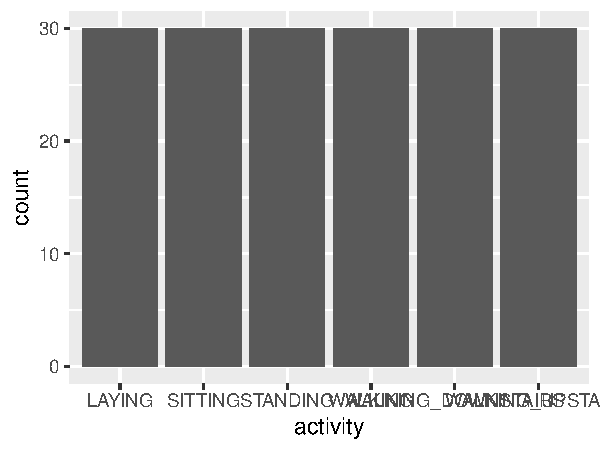
\includegraphics{codebook_tidydatasub_files/figure-latex/Var-1-activity-1.pdf}

\end{minipage}

\begin{itemize}
\tightlist
\item
  Observed factor levels: "LAYING", "SITTING", "STANDING", "WALKING",
  "WALKING\_DOWNSTAIRS", "WALKING\_UPSTAIRS".
\end{itemize}

\noindent\makebox[\linewidth]{\rule{\textwidth}{0.4pt}}

\hypertarget{subject}{%
\subsection{subject}\label{subject}}

\begin{minipage}{0.75 \textwidth}

\begin{longtable}[]{@{}lr@{}}
\toprule
\begin{minipage}[b]{0.34\columnwidth}\raggedright
Feature\strut
\end{minipage} & \begin{minipage}[b]{0.13\columnwidth}\raggedleft
Result\strut
\end{minipage}\tabularnewline
\midrule
\endhead
\begin{minipage}[t]{0.34\columnwidth}\raggedright
Variable type\strut
\end{minipage} & \begin{minipage}[t]{0.13\columnwidth}\raggedleft
integer\strut
\end{minipage}\tabularnewline
\begin{minipage}[t]{0.34\columnwidth}\raggedright
Number of missing obs.\strut
\end{minipage} & \begin{minipage}[t]{0.13\columnwidth}\raggedleft
0 (0 \%)\strut
\end{minipage}\tabularnewline
\begin{minipage}[t]{0.34\columnwidth}\raggedright
Number of unique values\strut
\end{minipage} & \begin{minipage}[t]{0.13\columnwidth}\raggedleft
30\strut
\end{minipage}\tabularnewline
\begin{minipage}[t]{0.34\columnwidth}\raggedright
Median\strut
\end{minipage} & \begin{minipage}[t]{0.13\columnwidth}\raggedleft
15.5\strut
\end{minipage}\tabularnewline
\begin{minipage}[t]{0.34\columnwidth}\raggedright
1st and 3rd quartiles\strut
\end{minipage} & \begin{minipage}[t]{0.13\columnwidth}\raggedleft
8; 23\strut
\end{minipage}\tabularnewline
\begin{minipage}[t]{0.34\columnwidth}\raggedright
Min. and max.\strut
\end{minipage} & \begin{minipage}[t]{0.13\columnwidth}\raggedleft
1; 30\strut
\end{minipage}\tabularnewline
\bottomrule
\end{longtable}

\end{minipage}
\begin{minipage}{0.25 \textwidth}

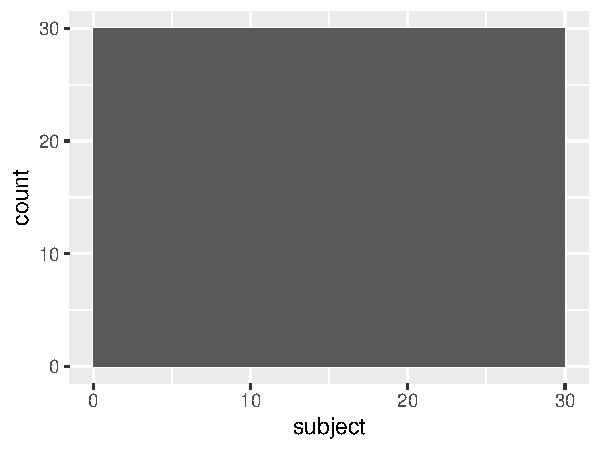
\includegraphics{codebook_tidydatasub_files/figure-latex/Var-2-subject-1.pdf}

\end{minipage}

\noindent\makebox[\linewidth]{\rule{\textwidth}{0.4pt}}

\hypertarget{timedomain_bodyacceleration_-mean--x}{%
\subsection{Timedomain\_BodyAcceleration\_-mean
-X}\label{timedomain_bodyacceleration_-mean--x}}

\begin{minipage}{0.75 \textwidth}

\begin{longtable}[]{@{}lr@{}}
\toprule
\begin{minipage}[b]{0.34\columnwidth}\raggedright
Feature\strut
\end{minipage} & \begin{minipage}[b]{0.17\columnwidth}\raggedleft
Result\strut
\end{minipage}\tabularnewline
\midrule
\endhead
\begin{minipage}[t]{0.34\columnwidth}\raggedright
Variable type\strut
\end{minipage} & \begin{minipage}[t]{0.17\columnwidth}\raggedleft
numeric\strut
\end{minipage}\tabularnewline
\begin{minipage}[t]{0.34\columnwidth}\raggedright
Number of missing obs.\strut
\end{minipage} & \begin{minipage}[t]{0.17\columnwidth}\raggedleft
0 (0 \%)\strut
\end{minipage}\tabularnewline
\begin{minipage}[t]{0.34\columnwidth}\raggedright
Number of unique values\strut
\end{minipage} & \begin{minipage}[t]{0.17\columnwidth}\raggedleft
180\strut
\end{minipage}\tabularnewline
\begin{minipage}[t]{0.34\columnwidth}\raggedright
Median\strut
\end{minipage} & \begin{minipage}[t]{0.17\columnwidth}\raggedleft
0.28\strut
\end{minipage}\tabularnewline
\begin{minipage}[t]{0.34\columnwidth}\raggedright
1st and 3rd quartiles\strut
\end{minipage} & \begin{minipage}[t]{0.17\columnwidth}\raggedleft
0.27; 0.28\strut
\end{minipage}\tabularnewline
\begin{minipage}[t]{0.34\columnwidth}\raggedright
Min. and max.\strut
\end{minipage} & \begin{minipage}[t]{0.17\columnwidth}\raggedleft
0.22; 0.3\strut
\end{minipage}\tabularnewline
\bottomrule
\end{longtable}

\end{minipage}
\begin{minipage}{0.25 \textwidth}

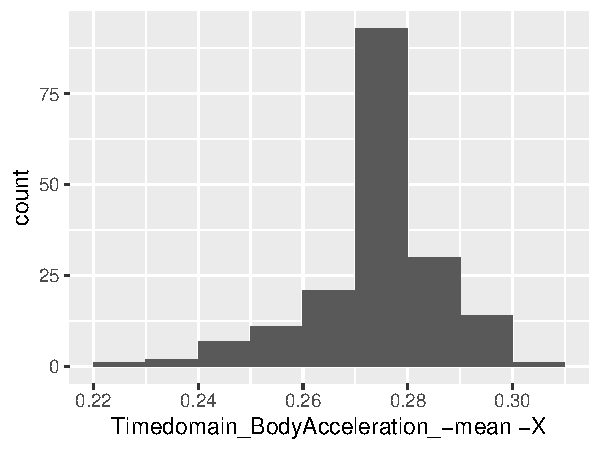
\includegraphics{codebook_tidydatasub_files/figure-latex/Var-3-Timedomain-BodyAcceleration--mean--X-1.pdf}

\end{minipage}

\noindent\makebox[\linewidth]{\rule{\textwidth}{0.4pt}}

\hypertarget{timedomain_bodyacceleration_-mean--y}{%
\subsection{Timedomain\_BodyAcceleration\_-mean
-Y}\label{timedomain_bodyacceleration_-mean--y}}

\begin{minipage}{0.75 \textwidth}

\begin{longtable}[]{@{}lr@{}}
\toprule
\begin{minipage}[b]{0.34\columnwidth}\raggedright
Feature\strut
\end{minipage} & \begin{minipage}[b]{0.20\columnwidth}\raggedleft
Result\strut
\end{minipage}\tabularnewline
\midrule
\endhead
\begin{minipage}[t]{0.34\columnwidth}\raggedright
Variable type\strut
\end{minipage} & \begin{minipage}[t]{0.20\columnwidth}\raggedleft
numeric\strut
\end{minipage}\tabularnewline
\begin{minipage}[t]{0.34\columnwidth}\raggedright
Number of missing obs.\strut
\end{minipage} & \begin{minipage}[t]{0.20\columnwidth}\raggedleft
0 (0 \%)\strut
\end{minipage}\tabularnewline
\begin{minipage}[t]{0.34\columnwidth}\raggedright
Number of unique values\strut
\end{minipage} & \begin{minipage}[t]{0.20\columnwidth}\raggedleft
180\strut
\end{minipage}\tabularnewline
\begin{minipage}[t]{0.34\columnwidth}\raggedright
Median\strut
\end{minipage} & \begin{minipage}[t]{0.20\columnwidth}\raggedleft
-0.02\strut
\end{minipage}\tabularnewline
\begin{minipage}[t]{0.34\columnwidth}\raggedright
1st and 3rd quartiles\strut
\end{minipage} & \begin{minipage}[t]{0.20\columnwidth}\raggedleft
-0.02; -0.01\strut
\end{minipage}\tabularnewline
\begin{minipage}[t]{0.34\columnwidth}\raggedright
Min. and max.\strut
\end{minipage} & \begin{minipage}[t]{0.20\columnwidth}\raggedleft
-0.04; 0\strut
\end{minipage}\tabularnewline
\bottomrule
\end{longtable}

\end{minipage}
\begin{minipage}{0.25 \textwidth}

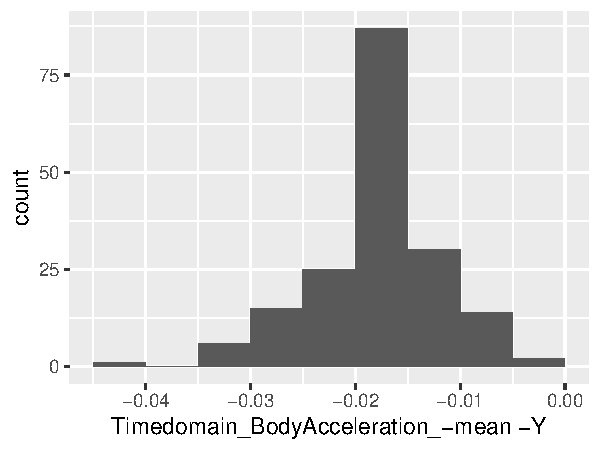
\includegraphics{codebook_tidydatasub_files/figure-latex/Var-4-Timedomain-BodyAcceleration--mean--Y-1.pdf}

\end{minipage}

\noindent\makebox[\linewidth]{\rule{\textwidth}{0.4pt}}

\hypertarget{timedomain_bodyacceleration_-mean--z}{%
\subsection{Timedomain\_BodyAcceleration\_-mean
-Z}\label{timedomain_bodyacceleration_-mean--z}}

\begin{minipage}{0.75 \textwidth}

\begin{longtable}[]{@{}lr@{}}
\toprule
\begin{minipage}[b]{0.34\columnwidth}\raggedright
Feature\strut
\end{minipage} & \begin{minipage}[b]{0.20\columnwidth}\raggedleft
Result\strut
\end{minipage}\tabularnewline
\midrule
\endhead
\begin{minipage}[t]{0.34\columnwidth}\raggedright
Variable type\strut
\end{minipage} & \begin{minipage}[t]{0.20\columnwidth}\raggedleft
numeric\strut
\end{minipage}\tabularnewline
\begin{minipage}[t]{0.34\columnwidth}\raggedright
Number of missing obs.\strut
\end{minipage} & \begin{minipage}[t]{0.20\columnwidth}\raggedleft
0 (0 \%)\strut
\end{minipage}\tabularnewline
\begin{minipage}[t]{0.34\columnwidth}\raggedright
Number of unique values\strut
\end{minipage} & \begin{minipage}[t]{0.20\columnwidth}\raggedleft
180\strut
\end{minipage}\tabularnewline
\begin{minipage}[t]{0.34\columnwidth}\raggedright
Median\strut
\end{minipage} & \begin{minipage}[t]{0.20\columnwidth}\raggedleft
-0.11\strut
\end{minipage}\tabularnewline
\begin{minipage}[t]{0.34\columnwidth}\raggedright
1st and 3rd quartiles\strut
\end{minipage} & \begin{minipage}[t]{0.20\columnwidth}\raggedleft
-0.11; -0.1\strut
\end{minipage}\tabularnewline
\begin{minipage}[t]{0.34\columnwidth}\raggedright
Min. and max.\strut
\end{minipage} & \begin{minipage}[t]{0.20\columnwidth}\raggedleft
-0.15; -0.08\strut
\end{minipage}\tabularnewline
\bottomrule
\end{longtable}

\end{minipage}
\begin{minipage}{0.25 \textwidth}

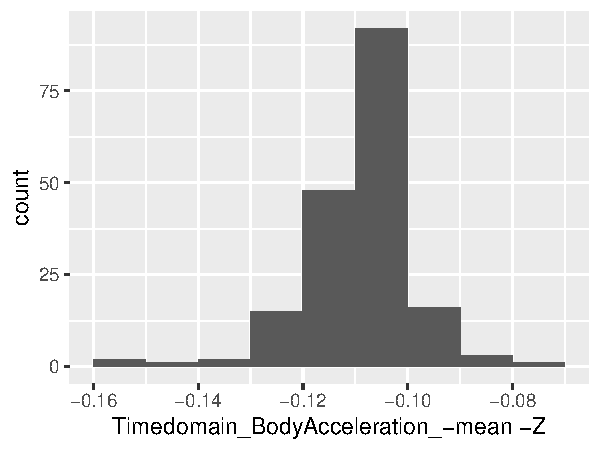
\includegraphics{codebook_tidydatasub_files/figure-latex/Var-5-Timedomain-BodyAcceleration--mean--Z-1.pdf}

\end{minipage}

\noindent\makebox[\linewidth]{\rule{\textwidth}{0.4pt}}

\hypertarget{timedomain_bodyacceleration_-standard-deviation--x}{%
\subsection{Timedomain\_BodyAcceleration\_-Standard-Deviation
-X}\label{timedomain_bodyacceleration_-standard-deviation--x}}

\begin{minipage}{0.75 \textwidth}

\begin{longtable}[]{@{}lr@{}}
\toprule
\begin{minipage}[b]{0.34\columnwidth}\raggedright
Feature\strut
\end{minipage} & \begin{minipage}[b]{0.18\columnwidth}\raggedleft
Result\strut
\end{minipage}\tabularnewline
\midrule
\endhead
\begin{minipage}[t]{0.34\columnwidth}\raggedright
Variable type\strut
\end{minipage} & \begin{minipage}[t]{0.18\columnwidth}\raggedleft
numeric\strut
\end{minipage}\tabularnewline
\begin{minipage}[t]{0.34\columnwidth}\raggedright
Number of missing obs.\strut
\end{minipage} & \begin{minipage}[t]{0.18\columnwidth}\raggedleft
0 (0 \%)\strut
\end{minipage}\tabularnewline
\begin{minipage}[t]{0.34\columnwidth}\raggedright
Number of unique values\strut
\end{minipage} & \begin{minipage}[t]{0.18\columnwidth}\raggedleft
180\strut
\end{minipage}\tabularnewline
\begin{minipage}[t]{0.34\columnwidth}\raggedright
Median\strut
\end{minipage} & \begin{minipage}[t]{0.18\columnwidth}\raggedleft
-0.75\strut
\end{minipage}\tabularnewline
\begin{minipage}[t]{0.34\columnwidth}\raggedright
1st and 3rd quartiles\strut
\end{minipage} & \begin{minipage}[t]{0.18\columnwidth}\raggedleft
-0.98; -0.2\strut
\end{minipage}\tabularnewline
\begin{minipage}[t]{0.34\columnwidth}\raggedright
Min. and max.\strut
\end{minipage} & \begin{minipage}[t]{0.18\columnwidth}\raggedleft
-1; 0.63\strut
\end{minipage}\tabularnewline
\bottomrule
\end{longtable}

\end{minipage}
\begin{minipage}{0.25 \textwidth}

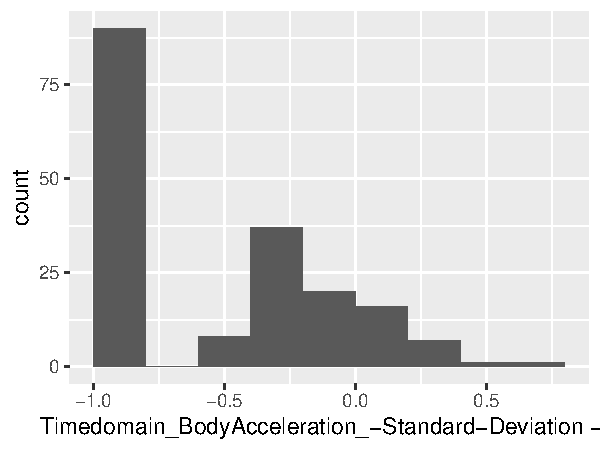
\includegraphics{codebook_tidydatasub_files/figure-latex/Var-6-Timedomain-BodyAcceleration--Standard-Deviation--X-1.pdf}

\end{minipage}

\noindent\makebox[\linewidth]{\rule{\textwidth}{0.4pt}}

\hypertarget{timedomain_bodyacceleration_-standard-deviation--y}{%
\subsection{Timedomain\_BodyAcceleration\_-Standard-Deviation
-Y}\label{timedomain_bodyacceleration_-standard-deviation--y}}

\begin{minipage}{0.75 \textwidth}

\begin{longtable}[]{@{}lr@{}}
\toprule
\begin{minipage}[b]{0.34\columnwidth}\raggedright
Feature\strut
\end{minipage} & \begin{minipage}[b]{0.20\columnwidth}\raggedleft
Result\strut
\end{minipage}\tabularnewline
\midrule
\endhead
\begin{minipage}[t]{0.34\columnwidth}\raggedright
Variable type\strut
\end{minipage} & \begin{minipage}[t]{0.20\columnwidth}\raggedleft
numeric\strut
\end{minipage}\tabularnewline
\begin{minipage}[t]{0.34\columnwidth}\raggedright
Number of missing obs.\strut
\end{minipage} & \begin{minipage}[t]{0.20\columnwidth}\raggedleft
0 (0 \%)\strut
\end{minipage}\tabularnewline
\begin{minipage}[t]{0.34\columnwidth}\raggedright
Number of unique values\strut
\end{minipage} & \begin{minipage}[t]{0.20\columnwidth}\raggedleft
180\strut
\end{minipage}\tabularnewline
\begin{minipage}[t]{0.34\columnwidth}\raggedright
Median\strut
\end{minipage} & \begin{minipage}[t]{0.20\columnwidth}\raggedleft
-0.51\strut
\end{minipage}\tabularnewline
\begin{minipage}[t]{0.34\columnwidth}\raggedright
1st and 3rd quartiles\strut
\end{minipage} & \begin{minipage}[t]{0.20\columnwidth}\raggedleft
-0.94; -0.03\strut
\end{minipage}\tabularnewline
\begin{minipage}[t]{0.34\columnwidth}\raggedright
Min. and max.\strut
\end{minipage} & \begin{minipage}[t]{0.20\columnwidth}\raggedleft
-0.99; 0.62\strut
\end{minipage}\tabularnewline
\bottomrule
\end{longtable}

\end{minipage}
\begin{minipage}{0.25 \textwidth}

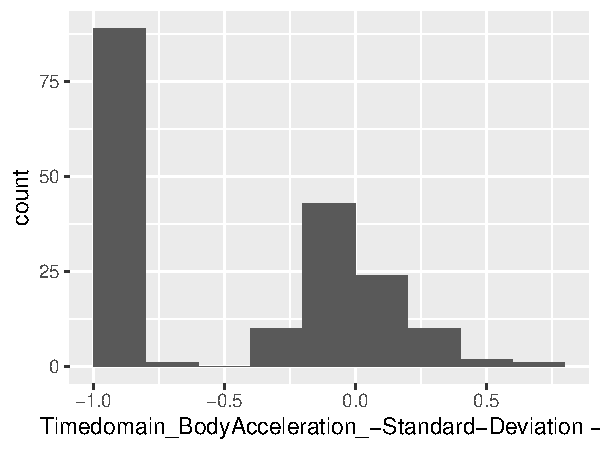
\includegraphics{codebook_tidydatasub_files/figure-latex/Var-7-Timedomain-BodyAcceleration--Standard-Deviation--Y-1.pdf}

\end{minipage}

\noindent\makebox[\linewidth]{\rule{\textwidth}{0.4pt}}

\hypertarget{timedomain_bodyacceleration_-standard-deviation--z}{%
\subsection{Timedomain\_BodyAcceleration\_-Standard-Deviation
-Z}\label{timedomain_bodyacceleration_-standard-deviation--z}}

\begin{minipage}{0.75 \textwidth}

\begin{longtable}[]{@{}lr@{}}
\toprule
\begin{minipage}[b]{0.34\columnwidth}\raggedright
Feature\strut
\end{minipage} & \begin{minipage}[b]{0.20\columnwidth}\raggedleft
Result\strut
\end{minipage}\tabularnewline
\midrule
\endhead
\begin{minipage}[t]{0.34\columnwidth}\raggedright
Variable type\strut
\end{minipage} & \begin{minipage}[t]{0.20\columnwidth}\raggedleft
numeric\strut
\end{minipage}\tabularnewline
\begin{minipage}[t]{0.34\columnwidth}\raggedright
Number of missing obs.\strut
\end{minipage} & \begin{minipage}[t]{0.20\columnwidth}\raggedleft
0 (0 \%)\strut
\end{minipage}\tabularnewline
\begin{minipage}[t]{0.34\columnwidth}\raggedright
Number of unique values\strut
\end{minipage} & \begin{minipage}[t]{0.20\columnwidth}\raggedleft
180\strut
\end{minipage}\tabularnewline
\begin{minipage}[t]{0.34\columnwidth}\raggedright
Median\strut
\end{minipage} & \begin{minipage}[t]{0.20\columnwidth}\raggedleft
-0.65\strut
\end{minipage}\tabularnewline
\begin{minipage}[t]{0.34\columnwidth}\raggedright
1st and 3rd quartiles\strut
\end{minipage} & \begin{minipage}[t]{0.20\columnwidth}\raggedleft
-0.95; -0.23\strut
\end{minipage}\tabularnewline
\begin{minipage}[t]{0.34\columnwidth}\raggedright
Min. and max.\strut
\end{minipage} & \begin{minipage}[t]{0.20\columnwidth}\raggedleft
-0.99; 0.61\strut
\end{minipage}\tabularnewline
\bottomrule
\end{longtable}

\end{minipage}
\begin{minipage}{0.25 \textwidth}

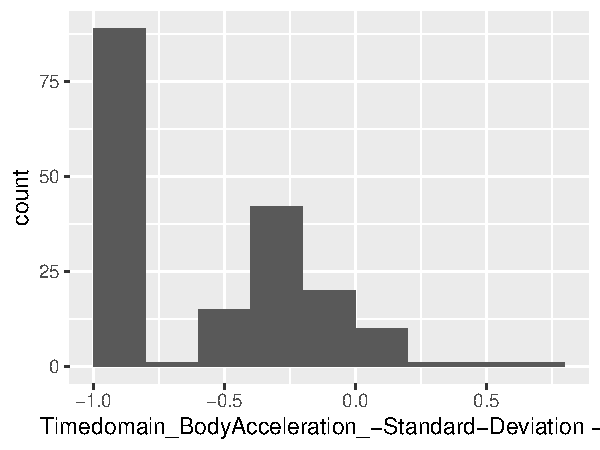
\includegraphics{codebook_tidydatasub_files/figure-latex/Var-8-Timedomain-BodyAcceleration--Standard-Deviation--Z-1.pdf}

\end{minipage}

\noindent\makebox[\linewidth]{\rule{\textwidth}{0.4pt}}

\hypertarget{timedomain_gravityacceleration_-mean--x}{%
\subsection{Timedomain\_GravityAcceleration\_-mean
-X}\label{timedomain_gravityacceleration_-mean--x}}

\begin{minipage}{0.75 \textwidth}

\begin{longtable}[]{@{}lr@{}}
\toprule
\begin{minipage}[b]{0.34\columnwidth}\raggedright
Feature\strut
\end{minipage} & \begin{minipage}[b]{0.18\columnwidth}\raggedleft
Result\strut
\end{minipage}\tabularnewline
\midrule
\endhead
\begin{minipage}[t]{0.34\columnwidth}\raggedright
Variable type\strut
\end{minipage} & \begin{minipage}[t]{0.18\columnwidth}\raggedleft
numeric\strut
\end{minipage}\tabularnewline
\begin{minipage}[t]{0.34\columnwidth}\raggedright
Number of missing obs.\strut
\end{minipage} & \begin{minipage}[t]{0.18\columnwidth}\raggedleft
0 (0 \%)\strut
\end{minipage}\tabularnewline
\begin{minipage}[t]{0.34\columnwidth}\raggedright
Number of unique values\strut
\end{minipage} & \begin{minipage}[t]{0.18\columnwidth}\raggedleft
180\strut
\end{minipage}\tabularnewline
\begin{minipage}[t]{0.34\columnwidth}\raggedright
Median\strut
\end{minipage} & \begin{minipage}[t]{0.18\columnwidth}\raggedleft
0.92\strut
\end{minipage}\tabularnewline
\begin{minipage}[t]{0.34\columnwidth}\raggedright
1st and 3rd quartiles\strut
\end{minipage} & \begin{minipage}[t]{0.18\columnwidth}\raggedleft
0.84; 0.94\strut
\end{minipage}\tabularnewline
\begin{minipage}[t]{0.34\columnwidth}\raggedright
Min. and max.\strut
\end{minipage} & \begin{minipage}[t]{0.18\columnwidth}\raggedleft
-0.68; 0.97\strut
\end{minipage}\tabularnewline
\bottomrule
\end{longtable}

\end{minipage}
\begin{minipage}{0.25 \textwidth}

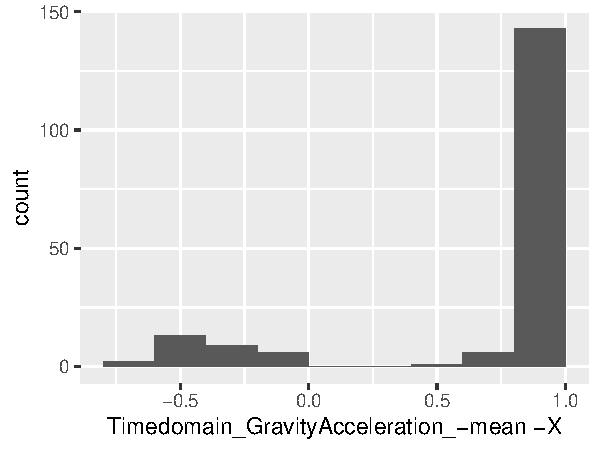
\includegraphics{codebook_tidydatasub_files/figure-latex/Var-9-Timedomain-GravityAcceleration--mean--X-1.pdf}

\end{minipage}

\noindent\makebox[\linewidth]{\rule{\textwidth}{0.4pt}}

\hypertarget{timedomain_gravityacceleration_-mean--y}{%
\subsection{Timedomain\_GravityAcceleration\_-mean
-Y}\label{timedomain_gravityacceleration_-mean--y}}

\begin{minipage}{0.75 \textwidth}

\begin{longtable}[]{@{}lr@{}}
\toprule
\begin{minipage}[b]{0.34\columnwidth}\raggedright
Feature\strut
\end{minipage} & \begin{minipage}[b]{0.18\columnwidth}\raggedleft
Result\strut
\end{minipage}\tabularnewline
\midrule
\endhead
\begin{minipage}[t]{0.34\columnwidth}\raggedright
Variable type\strut
\end{minipage} & \begin{minipage}[t]{0.18\columnwidth}\raggedleft
numeric\strut
\end{minipage}\tabularnewline
\begin{minipage}[t]{0.34\columnwidth}\raggedright
Number of missing obs.\strut
\end{minipage} & \begin{minipage}[t]{0.18\columnwidth}\raggedleft
0 (0 \%)\strut
\end{minipage}\tabularnewline
\begin{minipage}[t]{0.34\columnwidth}\raggedright
Number of unique values\strut
\end{minipage} & \begin{minipage}[t]{0.18\columnwidth}\raggedleft
180\strut
\end{minipage}\tabularnewline
\begin{minipage}[t]{0.34\columnwidth}\raggedright
Median\strut
\end{minipage} & \begin{minipage}[t]{0.18\columnwidth}\raggedleft
-0.13\strut
\end{minipage}\tabularnewline
\begin{minipage}[t]{0.34\columnwidth}\raggedright
1st and 3rd quartiles\strut
\end{minipage} & \begin{minipage}[t]{0.18\columnwidth}\raggedleft
-0.23; 0.09\strut
\end{minipage}\tabularnewline
\begin{minipage}[t]{0.34\columnwidth}\raggedright
Min. and max.\strut
\end{minipage} & \begin{minipage}[t]{0.18\columnwidth}\raggedleft
-0.48; 0.96\strut
\end{minipage}\tabularnewline
\bottomrule
\end{longtable}

\end{minipage}
\begin{minipage}{0.25 \textwidth}

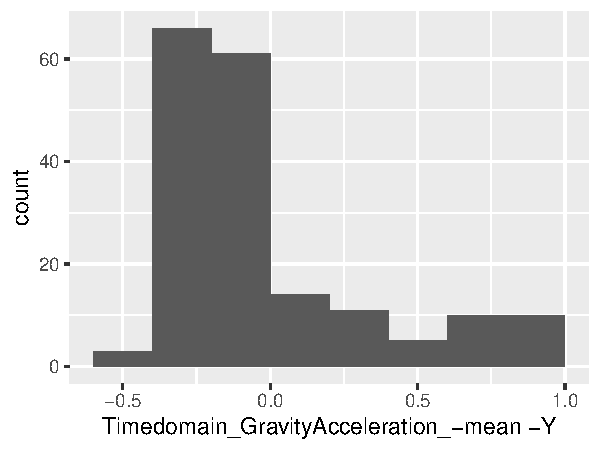
\includegraphics{codebook_tidydatasub_files/figure-latex/Var-10-Timedomain-GravityAcceleration--mean--Y-1.pdf}

\end{minipage}

\noindent\makebox[\linewidth]{\rule{\textwidth}{0.4pt}}

\hypertarget{timedomain_gravityacceleration_-mean--z}{%
\subsection{Timedomain\_GravityAcceleration\_-mean
-Z}\label{timedomain_gravityacceleration_-mean--z}}

\begin{minipage}{0.75 \textwidth}

\begin{longtable}[]{@{}lr@{}}
\toprule
\begin{minipage}[b]{0.34\columnwidth}\raggedright
Feature\strut
\end{minipage} & \begin{minipage}[b]{0.18\columnwidth}\raggedleft
Result\strut
\end{minipage}\tabularnewline
\midrule
\endhead
\begin{minipage}[t]{0.34\columnwidth}\raggedright
Variable type\strut
\end{minipage} & \begin{minipage}[t]{0.18\columnwidth}\raggedleft
numeric\strut
\end{minipage}\tabularnewline
\begin{minipage}[t]{0.34\columnwidth}\raggedright
Number of missing obs.\strut
\end{minipage} & \begin{minipage}[t]{0.18\columnwidth}\raggedleft
0 (0 \%)\strut
\end{minipage}\tabularnewline
\begin{minipage}[t]{0.34\columnwidth}\raggedright
Number of unique values\strut
\end{minipage} & \begin{minipage}[t]{0.18\columnwidth}\raggedleft
180\strut
\end{minipage}\tabularnewline
\begin{minipage}[t]{0.34\columnwidth}\raggedright
Median\strut
\end{minipage} & \begin{minipage}[t]{0.18\columnwidth}\raggedleft
0.02\strut
\end{minipage}\tabularnewline
\begin{minipage}[t]{0.34\columnwidth}\raggedright
1st and 3rd quartiles\strut
\end{minipage} & \begin{minipage}[t]{0.18\columnwidth}\raggedleft
-0.12; 0.15\strut
\end{minipage}\tabularnewline
\begin{minipage}[t]{0.34\columnwidth}\raggedright
Min. and max.\strut
\end{minipage} & \begin{minipage}[t]{0.18\columnwidth}\raggedleft
-0.5; 0.96\strut
\end{minipage}\tabularnewline
\bottomrule
\end{longtable}

\end{minipage}
\begin{minipage}{0.25 \textwidth}

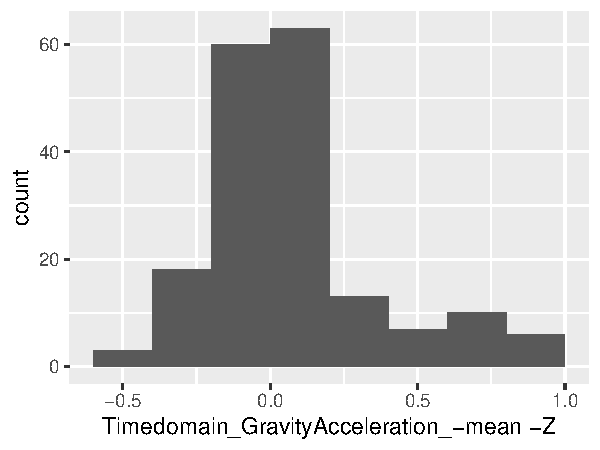
\includegraphics{codebook_tidydatasub_files/figure-latex/Var-11-Timedomain-GravityAcceleration--mean--Z-1.pdf}

\end{minipage}

\noindent\makebox[\linewidth]{\rule{\textwidth}{0.4pt}}

\hypertarget{timedomain_gravityacceleration_-standard-deviation--x}{%
\subsection{Timedomain\_GravityAcceleration\_-Standard-Deviation
-X}\label{timedomain_gravityacceleration_-standard-deviation--x}}

\begin{minipage}{0.75 \textwidth}

\begin{longtable}[]{@{}lr@{}}
\toprule
\begin{minipage}[b]{0.34\columnwidth}\raggedright
Feature\strut
\end{minipage} & \begin{minipage}[b]{0.20\columnwidth}\raggedleft
Result\strut
\end{minipage}\tabularnewline
\midrule
\endhead
\begin{minipage}[t]{0.34\columnwidth}\raggedright
Variable type\strut
\end{minipage} & \begin{minipage}[t]{0.20\columnwidth}\raggedleft
numeric\strut
\end{minipage}\tabularnewline
\begin{minipage}[t]{0.34\columnwidth}\raggedright
Number of missing obs.\strut
\end{minipage} & \begin{minipage}[t]{0.20\columnwidth}\raggedleft
0 (0 \%)\strut
\end{minipage}\tabularnewline
\begin{minipage}[t]{0.34\columnwidth}\raggedright
Number of unique values\strut
\end{minipage} & \begin{minipage}[t]{0.20\columnwidth}\raggedleft
180\strut
\end{minipage}\tabularnewline
\begin{minipage}[t]{0.34\columnwidth}\raggedright
Median\strut
\end{minipage} & \begin{minipage}[t]{0.20\columnwidth}\raggedleft
-0.97\strut
\end{minipage}\tabularnewline
\begin{minipage}[t]{0.34\columnwidth}\raggedright
1st and 3rd quartiles\strut
\end{minipage} & \begin{minipage}[t]{0.20\columnwidth}\raggedleft
-0.98; -0.95\strut
\end{minipage}\tabularnewline
\begin{minipage}[t]{0.34\columnwidth}\raggedright
Min. and max.\strut
\end{minipage} & \begin{minipage}[t]{0.20\columnwidth}\raggedleft
-1; -0.83\strut
\end{minipage}\tabularnewline
\bottomrule
\end{longtable}

\end{minipage}
\begin{minipage}{0.25 \textwidth}

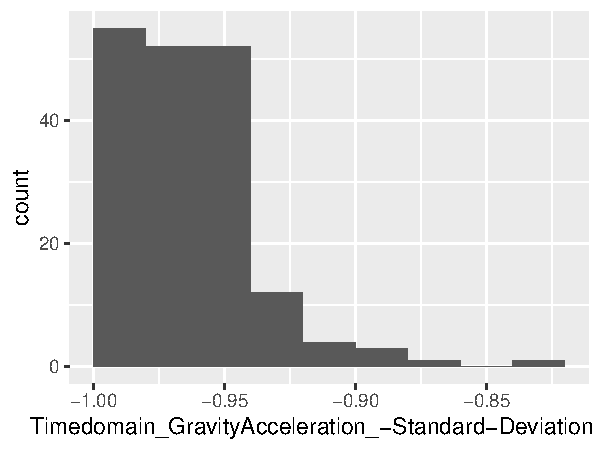
\includegraphics{codebook_tidydatasub_files/figure-latex/Var-12-Timedomain-GravityAcceleration--Standard-Deviation--X-1.pdf}

\end{minipage}

\noindent\makebox[\linewidth]{\rule{\textwidth}{0.4pt}}

\hypertarget{timedomain_gravityacceleration_-standard-deviation--y}{%
\subsection{Timedomain\_GravityAcceleration\_-Standard-Deviation
-Y}\label{timedomain_gravityacceleration_-standard-deviation--y}}

\begin{minipage}{0.75 \textwidth}

\begin{longtable}[]{@{}lr@{}}
\toprule
\begin{minipage}[b]{0.34\columnwidth}\raggedright
Feature\strut
\end{minipage} & \begin{minipage}[b]{0.20\columnwidth}\raggedleft
Result\strut
\end{minipage}\tabularnewline
\midrule
\endhead
\begin{minipage}[t]{0.34\columnwidth}\raggedright
Variable type\strut
\end{minipage} & \begin{minipage}[t]{0.20\columnwidth}\raggedleft
numeric\strut
\end{minipage}\tabularnewline
\begin{minipage}[t]{0.34\columnwidth}\raggedright
Number of missing obs.\strut
\end{minipage} & \begin{minipage}[t]{0.20\columnwidth}\raggedleft
0 (0 \%)\strut
\end{minipage}\tabularnewline
\begin{minipage}[t]{0.34\columnwidth}\raggedright
Number of unique values\strut
\end{minipage} & \begin{minipage}[t]{0.20\columnwidth}\raggedleft
180\strut
\end{minipage}\tabularnewline
\begin{minipage}[t]{0.34\columnwidth}\raggedright
Median\strut
\end{minipage} & \begin{minipage}[t]{0.20\columnwidth}\raggedleft
-0.96\strut
\end{minipage}\tabularnewline
\begin{minipage}[t]{0.34\columnwidth}\raggedright
1st and 3rd quartiles\strut
\end{minipage} & \begin{minipage}[t]{0.20\columnwidth}\raggedleft
-0.97; -0.94\strut
\end{minipage}\tabularnewline
\begin{minipage}[t]{0.34\columnwidth}\raggedright
Min. and max.\strut
\end{minipage} & \begin{minipage}[t]{0.20\columnwidth}\raggedleft
-0.99; -0.64\strut
\end{minipage}\tabularnewline
\bottomrule
\end{longtable}

\end{minipage}
\begin{minipage}{0.25 \textwidth}

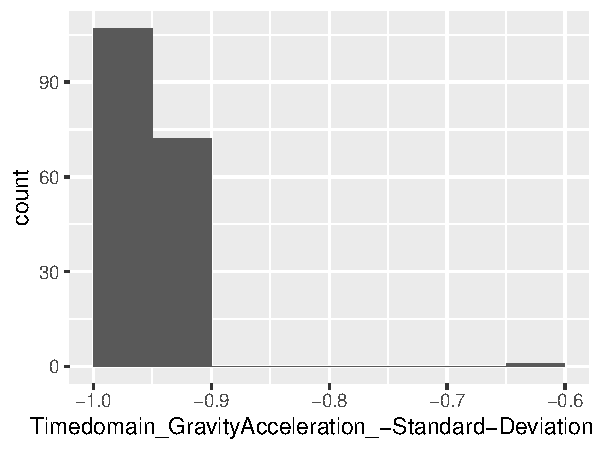
\includegraphics{codebook_tidydatasub_files/figure-latex/Var-13-Timedomain-GravityAcceleration--Standard-Deviation--Y-1.pdf}

\end{minipage}

\noindent\makebox[\linewidth]{\rule{\textwidth}{0.4pt}}

\hypertarget{timedomain_gravityacceleration_-standard-deviation--z}{%
\subsection{Timedomain\_GravityAcceleration\_-Standard-Deviation
-Z}\label{timedomain_gravityacceleration_-standard-deviation--z}}

\begin{minipage}{0.75 \textwidth}

\begin{longtable}[]{@{}lr@{}}
\toprule
\begin{minipage}[b]{0.34\columnwidth}\raggedright
Feature\strut
\end{minipage} & \begin{minipage}[b]{0.20\columnwidth}\raggedleft
Result\strut
\end{minipage}\tabularnewline
\midrule
\endhead
\begin{minipage}[t]{0.34\columnwidth}\raggedright
Variable type\strut
\end{minipage} & \begin{minipage}[t]{0.20\columnwidth}\raggedleft
numeric\strut
\end{minipage}\tabularnewline
\begin{minipage}[t]{0.34\columnwidth}\raggedright
Number of missing obs.\strut
\end{minipage} & \begin{minipage}[t]{0.20\columnwidth}\raggedleft
0 (0 \%)\strut
\end{minipage}\tabularnewline
\begin{minipage}[t]{0.34\columnwidth}\raggedright
Number of unique values\strut
\end{minipage} & \begin{minipage}[t]{0.20\columnwidth}\raggedleft
180\strut
\end{minipage}\tabularnewline
\begin{minipage}[t]{0.34\columnwidth}\raggedright
Median\strut
\end{minipage} & \begin{minipage}[t]{0.20\columnwidth}\raggedleft
-0.95\strut
\end{minipage}\tabularnewline
\begin{minipage}[t]{0.34\columnwidth}\raggedright
1st and 3rd quartiles\strut
\end{minipage} & \begin{minipage}[t]{0.20\columnwidth}\raggedleft
-0.96; -0.92\strut
\end{minipage}\tabularnewline
\begin{minipage}[t]{0.34\columnwidth}\raggedright
Min. and max.\strut
\end{minipage} & \begin{minipage}[t]{0.20\columnwidth}\raggedleft
-0.99; -0.61\strut
\end{minipage}\tabularnewline
\bottomrule
\end{longtable}

\end{minipage}
\begin{minipage}{0.25 \textwidth}

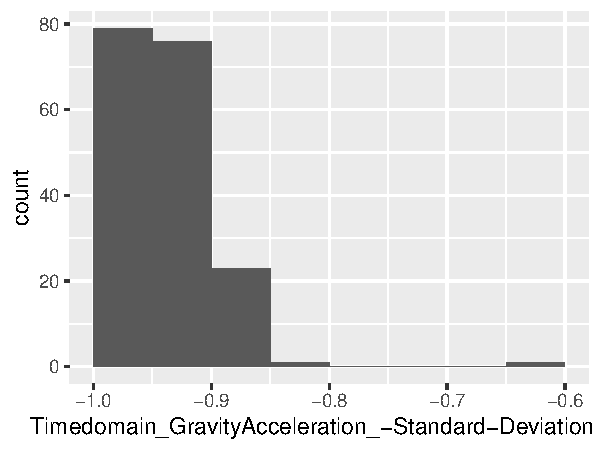
\includegraphics{codebook_tidydatasub_files/figure-latex/Var-14-Timedomain-GravityAcceleration--Standard-Deviation--Z-1.pdf}

\end{minipage}

\noindent\makebox[\linewidth]{\rule{\textwidth}{0.4pt}}

\hypertarget{timedomain_bodyacceleration_jerk-mean--x}{%
\subsection{Timedomain\_BodyAcceleration\_Jerk-mean
-X}\label{timedomain_bodyacceleration_jerk-mean--x}}

\begin{minipage}{0.75 \textwidth}

\begin{longtable}[]{@{}lr@{}}
\toprule
\begin{minipage}[b]{0.34\columnwidth}\raggedright
Feature\strut
\end{minipage} & \begin{minipage}[b]{0.17\columnwidth}\raggedleft
Result\strut
\end{minipage}\tabularnewline
\midrule
\endhead
\begin{minipage}[t]{0.34\columnwidth}\raggedright
Variable type\strut
\end{minipage} & \begin{minipage}[t]{0.17\columnwidth}\raggedleft
numeric\strut
\end{minipage}\tabularnewline
\begin{minipage}[t]{0.34\columnwidth}\raggedright
Number of missing obs.\strut
\end{minipage} & \begin{minipage}[t]{0.17\columnwidth}\raggedleft
0 (0 \%)\strut
\end{minipage}\tabularnewline
\begin{minipage}[t]{0.34\columnwidth}\raggedright
Number of unique values\strut
\end{minipage} & \begin{minipage}[t]{0.17\columnwidth}\raggedleft
180\strut
\end{minipage}\tabularnewline
\begin{minipage}[t]{0.34\columnwidth}\raggedright
Median\strut
\end{minipage} & \begin{minipage}[t]{0.17\columnwidth}\raggedleft
0.08\strut
\end{minipage}\tabularnewline
\begin{minipage}[t]{0.34\columnwidth}\raggedright
1st and 3rd quartiles\strut
\end{minipage} & \begin{minipage}[t]{0.17\columnwidth}\raggedleft
0.07; 0.08\strut
\end{minipage}\tabularnewline
\begin{minipage}[t]{0.34\columnwidth}\raggedright
Min. and max.\strut
\end{minipage} & \begin{minipage}[t]{0.17\columnwidth}\raggedleft
0.04; 0.13\strut
\end{minipage}\tabularnewline
\bottomrule
\end{longtable}

\end{minipage}
\begin{minipage}{0.25 \textwidth}

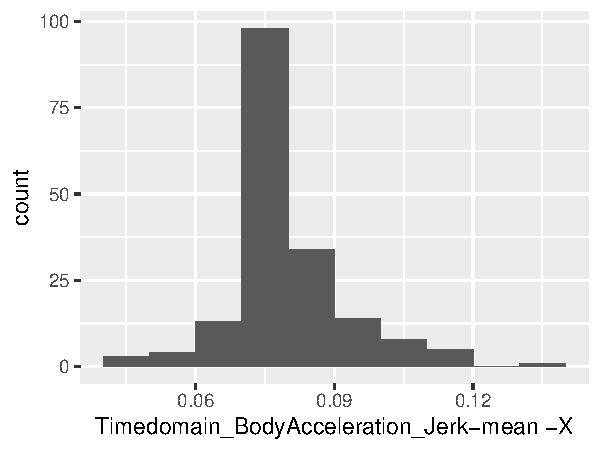
\includegraphics{codebook_tidydatasub_files/figure-latex/Var-15-Timedomain-BodyAcceleration-Jerk-mean--X-1.pdf}

\end{minipage}

\noindent\makebox[\linewidth]{\rule{\textwidth}{0.4pt}}

\hypertarget{timedomain_bodyacceleration_jerk-mean--y}{%
\subsection{Timedomain\_BodyAcceleration\_Jerk-mean
-Y}\label{timedomain_bodyacceleration_jerk-mean--y}}

\begin{minipage}{0.75 \textwidth}

\begin{longtable}[]{@{}lr@{}}
\toprule
\begin{minipage}[b]{0.34\columnwidth}\raggedright
Feature\strut
\end{minipage} & \begin{minipage}[b]{0.18\columnwidth}\raggedleft
Result\strut
\end{minipage}\tabularnewline
\midrule
\endhead
\begin{minipage}[t]{0.34\columnwidth}\raggedright
Variable type\strut
\end{minipage} & \begin{minipage}[t]{0.18\columnwidth}\raggedleft
numeric\strut
\end{minipage}\tabularnewline
\begin{minipage}[t]{0.34\columnwidth}\raggedright
Number of missing obs.\strut
\end{minipage} & \begin{minipage}[t]{0.18\columnwidth}\raggedleft
0 (0 \%)\strut
\end{minipage}\tabularnewline
\begin{minipage}[t]{0.34\columnwidth}\raggedright
Number of unique values\strut
\end{minipage} & \begin{minipage}[t]{0.18\columnwidth}\raggedleft
180\strut
\end{minipage}\tabularnewline
\begin{minipage}[t]{0.34\columnwidth}\raggedright
Median\strut
\end{minipage} & \begin{minipage}[t]{0.18\columnwidth}\raggedleft
0.01\strut
\end{minipage}\tabularnewline
\begin{minipage}[t]{0.34\columnwidth}\raggedright
1st and 3rd quartiles\strut
\end{minipage} & \begin{minipage}[t]{0.18\columnwidth}\raggedleft
0; 0.01\strut
\end{minipage}\tabularnewline
\begin{minipage}[t]{0.34\columnwidth}\raggedright
Min. and max.\strut
\end{minipage} & \begin{minipage}[t]{0.18\columnwidth}\raggedleft
-0.04; 0.06\strut
\end{minipage}\tabularnewline
\bottomrule
\end{longtable}

\end{minipage}
\begin{minipage}{0.25 \textwidth}

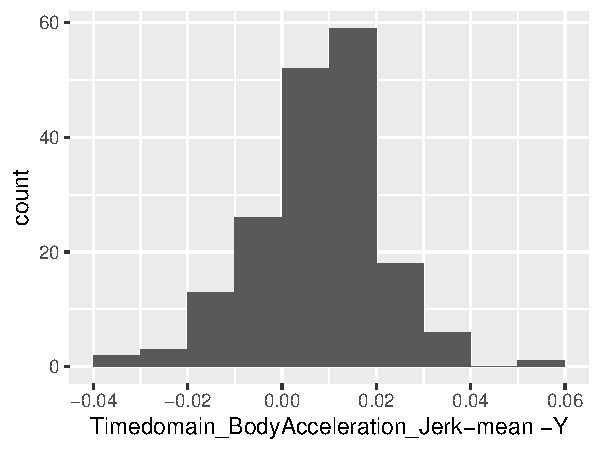
\includegraphics{codebook_tidydatasub_files/figure-latex/Var-16-Timedomain-BodyAcceleration-Jerk-mean--Y-1.pdf}

\end{minipage}

\noindent\makebox[\linewidth]{\rule{\textwidth}{0.4pt}}

\hypertarget{timedomain_bodyacceleration_jerk-mean--z}{%
\subsection{Timedomain\_BodyAcceleration\_Jerk-mean
-Z}\label{timedomain_bodyacceleration_jerk-mean--z}}

\begin{minipage}{0.75 \textwidth}

\begin{longtable}[]{@{}lr@{}}
\toprule
\begin{minipage}[b]{0.34\columnwidth}\raggedright
Feature\strut
\end{minipage} & \begin{minipage}[b]{0.18\columnwidth}\raggedleft
Result\strut
\end{minipage}\tabularnewline
\midrule
\endhead
\begin{minipage}[t]{0.34\columnwidth}\raggedright
Variable type\strut
\end{minipage} & \begin{minipage}[t]{0.18\columnwidth}\raggedleft
numeric\strut
\end{minipage}\tabularnewline
\begin{minipage}[t]{0.34\columnwidth}\raggedright
Number of missing obs.\strut
\end{minipage} & \begin{minipage}[t]{0.18\columnwidth}\raggedleft
0 (0 \%)\strut
\end{minipage}\tabularnewline
\begin{minipage}[t]{0.34\columnwidth}\raggedright
Number of unique values\strut
\end{minipage} & \begin{minipage}[t]{0.18\columnwidth}\raggedleft
180\strut
\end{minipage}\tabularnewline
\begin{minipage}[t]{0.34\columnwidth}\raggedright
Median\strut
\end{minipage} & \begin{minipage}[t]{0.18\columnwidth}\raggedleft
0\strut
\end{minipage}\tabularnewline
\begin{minipage}[t]{0.34\columnwidth}\raggedright
1st and 3rd quartiles\strut
\end{minipage} & \begin{minipage}[t]{0.18\columnwidth}\raggedleft
-0.01; 0\strut
\end{minipage}\tabularnewline
\begin{minipage}[t]{0.34\columnwidth}\raggedright
Min. and max.\strut
\end{minipage} & \begin{minipage}[t]{0.18\columnwidth}\raggedleft
-0.07; 0.04\strut
\end{minipage}\tabularnewline
\bottomrule
\end{longtable}

\end{minipage}
\begin{minipage}{0.25 \textwidth}

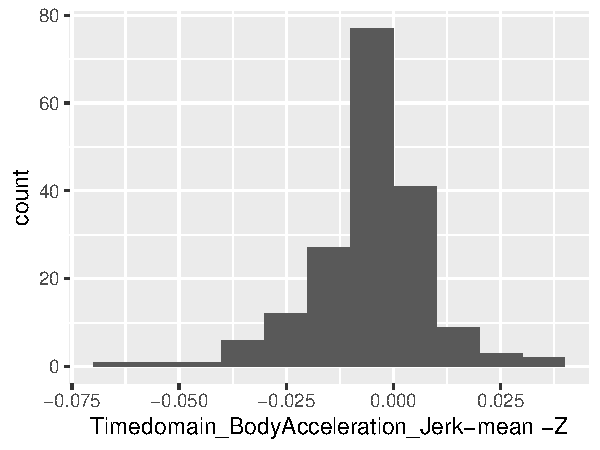
\includegraphics{codebook_tidydatasub_files/figure-latex/Var-17-Timedomain-BodyAcceleration-Jerk-mean--Z-1.pdf}

\end{minipage}

\noindent\makebox[\linewidth]{\rule{\textwidth}{0.4pt}}

\hypertarget{timedomain_bodyacceleration_jerk-standard-deviation--x}{%
\subsection{Timedomain\_BodyAcceleration\_Jerk-Standard-Deviation
-X}\label{timedomain_bodyacceleration_jerk-standard-deviation--x}}

\begin{minipage}{0.75 \textwidth}

\begin{longtable}[]{@{}lr@{}}
\toprule
\begin{minipage}[b]{0.34\columnwidth}\raggedright
Feature\strut
\end{minipage} & \begin{minipage}[b]{0.20\columnwidth}\raggedleft
Result\strut
\end{minipage}\tabularnewline
\midrule
\endhead
\begin{minipage}[t]{0.34\columnwidth}\raggedright
Variable type\strut
\end{minipage} & \begin{minipage}[t]{0.20\columnwidth}\raggedleft
numeric\strut
\end{minipage}\tabularnewline
\begin{minipage}[t]{0.34\columnwidth}\raggedright
Number of missing obs.\strut
\end{minipage} & \begin{minipage}[t]{0.20\columnwidth}\raggedleft
0 (0 \%)\strut
\end{minipage}\tabularnewline
\begin{minipage}[t]{0.34\columnwidth}\raggedright
Number of unique values\strut
\end{minipage} & \begin{minipage}[t]{0.20\columnwidth}\raggedleft
180\strut
\end{minipage}\tabularnewline
\begin{minipage}[t]{0.34\columnwidth}\raggedright
Median\strut
\end{minipage} & \begin{minipage}[t]{0.20\columnwidth}\raggedleft
-0.81\strut
\end{minipage}\tabularnewline
\begin{minipage}[t]{0.34\columnwidth}\raggedright
1st and 3rd quartiles\strut
\end{minipage} & \begin{minipage}[t]{0.20\columnwidth}\raggedleft
-0.98; -0.22\strut
\end{minipage}\tabularnewline
\begin{minipage}[t]{0.34\columnwidth}\raggedright
Min. and max.\strut
\end{minipage} & \begin{minipage}[t]{0.20\columnwidth}\raggedleft
-0.99; 0.54\strut
\end{minipage}\tabularnewline
\bottomrule
\end{longtable}

\end{minipage}
\begin{minipage}{0.25 \textwidth}

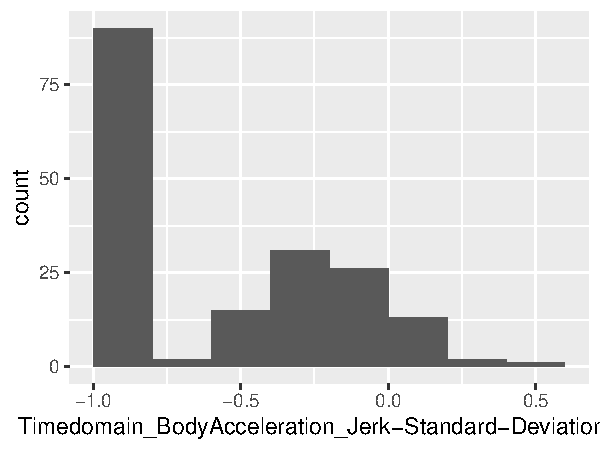
\includegraphics{codebook_tidydatasub_files/figure-latex/Var-18-Timedomain-BodyAcceleration-Jerk-Standard-Deviation--X-1.pdf}

\end{minipage}

\noindent\makebox[\linewidth]{\rule{\textwidth}{0.4pt}}

\hypertarget{timedomain_bodyacceleration_jerk-standard-deviation--y}{%
\subsection{Timedomain\_BodyAcceleration\_Jerk-Standard-Deviation
-Y}\label{timedomain_bodyacceleration_jerk-standard-deviation--y}}

\begin{minipage}{0.75 \textwidth}

\begin{longtable}[]{@{}lr@{}}
\toprule
\begin{minipage}[b]{0.34\columnwidth}\raggedright
Feature\strut
\end{minipage} & \begin{minipage}[b]{0.20\columnwidth}\raggedleft
Result\strut
\end{minipage}\tabularnewline
\midrule
\endhead
\begin{minipage}[t]{0.34\columnwidth}\raggedright
Variable type\strut
\end{minipage} & \begin{minipage}[t]{0.20\columnwidth}\raggedleft
numeric\strut
\end{minipage}\tabularnewline
\begin{minipage}[t]{0.34\columnwidth}\raggedright
Number of missing obs.\strut
\end{minipage} & \begin{minipage}[t]{0.20\columnwidth}\raggedleft
0 (0 \%)\strut
\end{minipage}\tabularnewline
\begin{minipage}[t]{0.34\columnwidth}\raggedright
Number of unique values\strut
\end{minipage} & \begin{minipage}[t]{0.20\columnwidth}\raggedleft
180\strut
\end{minipage}\tabularnewline
\begin{minipage}[t]{0.34\columnwidth}\raggedright
Median\strut
\end{minipage} & \begin{minipage}[t]{0.20\columnwidth}\raggedleft
-0.78\strut
\end{minipage}\tabularnewline
\begin{minipage}[t]{0.34\columnwidth}\raggedright
1st and 3rd quartiles\strut
\end{minipage} & \begin{minipage}[t]{0.20\columnwidth}\raggedleft
-0.97; -0.15\strut
\end{minipage}\tabularnewline
\begin{minipage}[t]{0.34\columnwidth}\raggedright
Min. and max.\strut
\end{minipage} & \begin{minipage}[t]{0.20\columnwidth}\raggedleft
-0.99; 0.36\strut
\end{minipage}\tabularnewline
\bottomrule
\end{longtable}

\end{minipage}
\begin{minipage}{0.25 \textwidth}

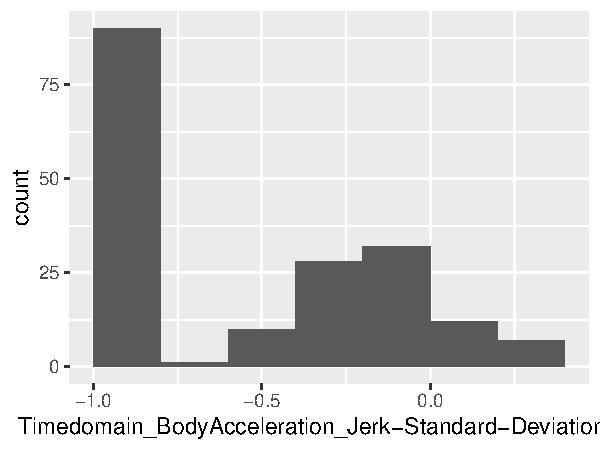
\includegraphics{codebook_tidydatasub_files/figure-latex/Var-19-Timedomain-BodyAcceleration-Jerk-Standard-Deviation--Y-1.pdf}

\end{minipage}

\noindent\makebox[\linewidth]{\rule{\textwidth}{0.4pt}}

\hypertarget{timedomain_bodyacceleration_jerk-standard-deviation--z}{%
\subsection{Timedomain\_BodyAcceleration\_Jerk-Standard-Deviation
-Z}\label{timedomain_bodyacceleration_jerk-standard-deviation--z}}

\begin{minipage}{0.75 \textwidth}

\begin{longtable}[]{@{}lr@{}}
\toprule
\begin{minipage}[b]{0.34\columnwidth}\raggedright
Feature\strut
\end{minipage} & \begin{minipage}[b]{0.20\columnwidth}\raggedleft
Result\strut
\end{minipage}\tabularnewline
\midrule
\endhead
\begin{minipage}[t]{0.34\columnwidth}\raggedright
Variable type\strut
\end{minipage} & \begin{minipage}[t]{0.20\columnwidth}\raggedleft
numeric\strut
\end{minipage}\tabularnewline
\begin{minipage}[t]{0.34\columnwidth}\raggedright
Number of missing obs.\strut
\end{minipage} & \begin{minipage}[t]{0.20\columnwidth}\raggedleft
0 (0 \%)\strut
\end{minipage}\tabularnewline
\begin{minipage}[t]{0.34\columnwidth}\raggedright
Number of unique values\strut
\end{minipage} & \begin{minipage}[t]{0.20\columnwidth}\raggedleft
180\strut
\end{minipage}\tabularnewline
\begin{minipage}[t]{0.34\columnwidth}\raggedright
Median\strut
\end{minipage} & \begin{minipage}[t]{0.20\columnwidth}\raggedleft
-0.88\strut
\end{minipage}\tabularnewline
\begin{minipage}[t]{0.34\columnwidth}\raggedright
1st and 3rd quartiles\strut
\end{minipage} & \begin{minipage}[t]{0.20\columnwidth}\raggedleft
-0.98; -0.51\strut
\end{minipage}\tabularnewline
\begin{minipage}[t]{0.34\columnwidth}\raggedright
Min. and max.\strut
\end{minipage} & \begin{minipage}[t]{0.20\columnwidth}\raggedleft
-0.99; 0.03\strut
\end{minipage}\tabularnewline
\bottomrule
\end{longtable}

\end{minipage}
\begin{minipage}{0.25 \textwidth}

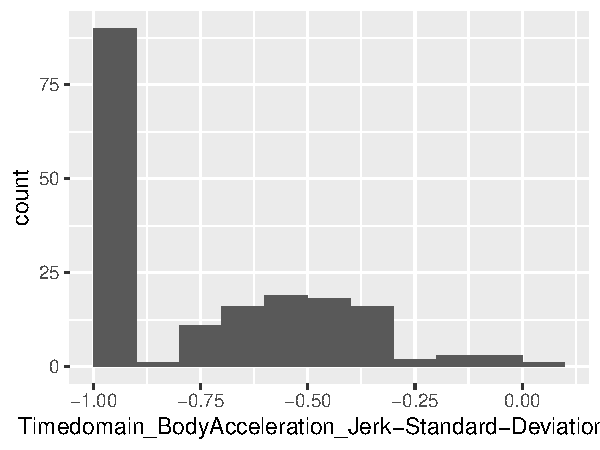
\includegraphics{codebook_tidydatasub_files/figure-latex/Var-20-Timedomain-BodyAcceleration-Jerk-Standard-Deviation--Z-1.pdf}

\end{minipage}

\noindent\makebox[\linewidth]{\rule{\textwidth}{0.4pt}}

\hypertarget{timedomain_bodygyroscope-mean--x}{%
\subsection{Timedomain\_BodyGyroscope-mean
-X}\label{timedomain_bodygyroscope-mean--x}}

\begin{minipage}{0.75 \textwidth}

\begin{longtable}[]{@{}lr@{}}
\toprule
\begin{minipage}[b]{0.34\columnwidth}\raggedright
Feature\strut
\end{minipage} & \begin{minipage}[b]{0.20\columnwidth}\raggedleft
Result\strut
\end{minipage}\tabularnewline
\midrule
\endhead
\begin{minipage}[t]{0.34\columnwidth}\raggedright
Variable type\strut
\end{minipage} & \begin{minipage}[t]{0.20\columnwidth}\raggedleft
numeric\strut
\end{minipage}\tabularnewline
\begin{minipage}[t]{0.34\columnwidth}\raggedright
Number of missing obs.\strut
\end{minipage} & \begin{minipage}[t]{0.20\columnwidth}\raggedleft
0 (0 \%)\strut
\end{minipage}\tabularnewline
\begin{minipage}[t]{0.34\columnwidth}\raggedright
Number of unique values\strut
\end{minipage} & \begin{minipage}[t]{0.20\columnwidth}\raggedleft
180\strut
\end{minipage}\tabularnewline
\begin{minipage}[t]{0.34\columnwidth}\raggedright
Median\strut
\end{minipage} & \begin{minipage}[t]{0.20\columnwidth}\raggedleft
-0.03\strut
\end{minipage}\tabularnewline
\begin{minipage}[t]{0.34\columnwidth}\raggedright
1st and 3rd quartiles\strut
\end{minipage} & \begin{minipage}[t]{0.20\columnwidth}\raggedleft
-0.05; -0.02\strut
\end{minipage}\tabularnewline
\begin{minipage}[t]{0.34\columnwidth}\raggedright
Min. and max.\strut
\end{minipage} & \begin{minipage}[t]{0.20\columnwidth}\raggedleft
-0.21; 0.19\strut
\end{minipage}\tabularnewline
\bottomrule
\end{longtable}

\end{minipage}
\begin{minipage}{0.25 \textwidth}

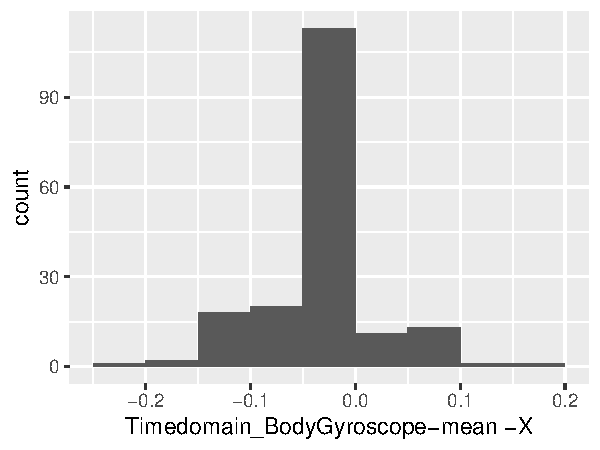
\includegraphics{codebook_tidydatasub_files/figure-latex/Var-21-Timedomain-BodyGyroscope-mean--X-1.pdf}

\end{minipage}

\noindent\makebox[\linewidth]{\rule{\textwidth}{0.4pt}}

\hypertarget{timedomain_bodygyroscope-mean--y}{%
\subsection{Timedomain\_BodyGyroscope-mean
-Y}\label{timedomain_bodygyroscope-mean--y}}

\begin{minipage}{0.75 \textwidth}

\begin{longtable}[]{@{}lr@{}}
\toprule
\begin{minipage}[b]{0.34\columnwidth}\raggedright
Feature\strut
\end{minipage} & \begin{minipage}[b]{0.20\columnwidth}\raggedleft
Result\strut
\end{minipage}\tabularnewline
\midrule
\endhead
\begin{minipage}[t]{0.34\columnwidth}\raggedright
Variable type\strut
\end{minipage} & \begin{minipage}[t]{0.20\columnwidth}\raggedleft
numeric\strut
\end{minipage}\tabularnewline
\begin{minipage}[t]{0.34\columnwidth}\raggedright
Number of missing obs.\strut
\end{minipage} & \begin{minipage}[t]{0.20\columnwidth}\raggedleft
0 (0 \%)\strut
\end{minipage}\tabularnewline
\begin{minipage}[t]{0.34\columnwidth}\raggedright
Number of unique values\strut
\end{minipage} & \begin{minipage}[t]{0.20\columnwidth}\raggedleft
180\strut
\end{minipage}\tabularnewline
\begin{minipage}[t]{0.34\columnwidth}\raggedright
Median\strut
\end{minipage} & \begin{minipage}[t]{0.20\columnwidth}\raggedleft
-0.07\strut
\end{minipage}\tabularnewline
\begin{minipage}[t]{0.34\columnwidth}\raggedright
1st and 3rd quartiles\strut
\end{minipage} & \begin{minipage}[t]{0.20\columnwidth}\raggedleft
-0.09; -0.06\strut
\end{minipage}\tabularnewline
\begin{minipage}[t]{0.34\columnwidth}\raggedright
Min. and max.\strut
\end{minipage} & \begin{minipage}[t]{0.20\columnwidth}\raggedleft
-0.2; 0.03\strut
\end{minipage}\tabularnewline
\bottomrule
\end{longtable}

\end{minipage}
\begin{minipage}{0.25 \textwidth}

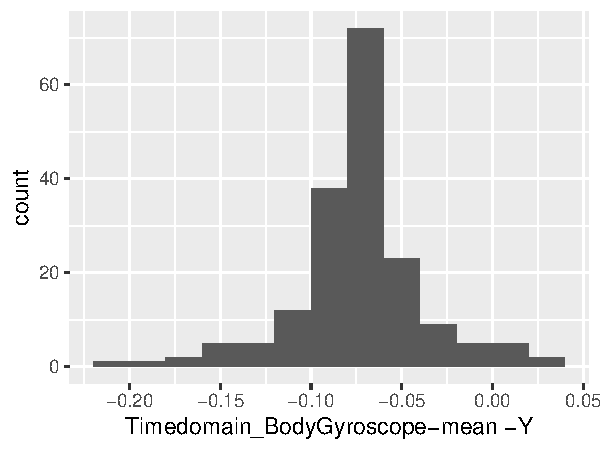
\includegraphics{codebook_tidydatasub_files/figure-latex/Var-22-Timedomain-BodyGyroscope-mean--Y-1.pdf}

\end{minipage}

\noindent\makebox[\linewidth]{\rule{\textwidth}{0.4pt}}

\hypertarget{timedomain_bodygyroscope-mean--z}{%
\subsection{Timedomain\_BodyGyroscope-mean
-Z}\label{timedomain_bodygyroscope-mean--z}}

\begin{minipage}{0.75 \textwidth}

\begin{longtable}[]{@{}lr@{}}
\toprule
\begin{minipage}[b]{0.34\columnwidth}\raggedright
Feature\strut
\end{minipage} & \begin{minipage}[b]{0.18\columnwidth}\raggedleft
Result\strut
\end{minipage}\tabularnewline
\midrule
\endhead
\begin{minipage}[t]{0.34\columnwidth}\raggedright
Variable type\strut
\end{minipage} & \begin{minipage}[t]{0.18\columnwidth}\raggedleft
numeric\strut
\end{minipage}\tabularnewline
\begin{minipage}[t]{0.34\columnwidth}\raggedright
Number of missing obs.\strut
\end{minipage} & \begin{minipage}[t]{0.18\columnwidth}\raggedleft
0 (0 \%)\strut
\end{minipage}\tabularnewline
\begin{minipage}[t]{0.34\columnwidth}\raggedright
Number of unique values\strut
\end{minipage} & \begin{minipage}[t]{0.18\columnwidth}\raggedleft
180\strut
\end{minipage}\tabularnewline
\begin{minipage}[t]{0.34\columnwidth}\raggedright
Median\strut
\end{minipage} & \begin{minipage}[t]{0.18\columnwidth}\raggedleft
0.09\strut
\end{minipage}\tabularnewline
\begin{minipage}[t]{0.34\columnwidth}\raggedright
1st and 3rd quartiles\strut
\end{minipage} & \begin{minipage}[t]{0.18\columnwidth}\raggedleft
0.07; 0.1\strut
\end{minipage}\tabularnewline
\begin{minipage}[t]{0.34\columnwidth}\raggedright
Min. and max.\strut
\end{minipage} & \begin{minipage}[t]{0.18\columnwidth}\raggedleft
-0.07; 0.18\strut
\end{minipage}\tabularnewline
\bottomrule
\end{longtable}

\end{minipage}
\begin{minipage}{0.25 \textwidth}

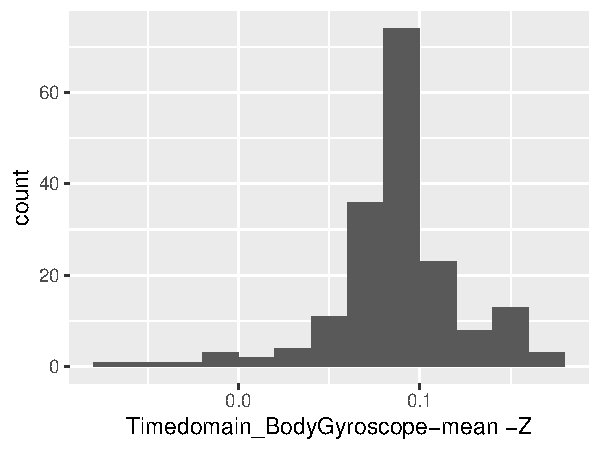
\includegraphics{codebook_tidydatasub_files/figure-latex/Var-23-Timedomain-BodyGyroscope-mean--Z-1.pdf}

\end{minipage}

\noindent\makebox[\linewidth]{\rule{\textwidth}{0.4pt}}

\hypertarget{timedomain_bodygyroscope-standard-deviation--x}{%
\subsection{Timedomain\_BodyGyroscope-Standard-Deviation
-X}\label{timedomain_bodygyroscope-standard-deviation--x}}

\begin{minipage}{0.75 \textwidth}

\begin{longtable}[]{@{}lr@{}}
\toprule
\begin{minipage}[b]{0.34\columnwidth}\raggedright
Feature\strut
\end{minipage} & \begin{minipage}[b]{0.20\columnwidth}\raggedleft
Result\strut
\end{minipage}\tabularnewline
\midrule
\endhead
\begin{minipage}[t]{0.34\columnwidth}\raggedright
Variable type\strut
\end{minipage} & \begin{minipage}[t]{0.20\columnwidth}\raggedleft
numeric\strut
\end{minipage}\tabularnewline
\begin{minipage}[t]{0.34\columnwidth}\raggedright
Number of missing obs.\strut
\end{minipage} & \begin{minipage}[t]{0.20\columnwidth}\raggedleft
0 (0 \%)\strut
\end{minipage}\tabularnewline
\begin{minipage}[t]{0.34\columnwidth}\raggedright
Number of unique values\strut
\end{minipage} & \begin{minipage}[t]{0.20\columnwidth}\raggedleft
180\strut
\end{minipage}\tabularnewline
\begin{minipage}[t]{0.34\columnwidth}\raggedright
Median\strut
\end{minipage} & \begin{minipage}[t]{0.20\columnwidth}\raggedleft
-0.79\strut
\end{minipage}\tabularnewline
\begin{minipage}[t]{0.34\columnwidth}\raggedright
1st and 3rd quartiles\strut
\end{minipage} & \begin{minipage}[t]{0.20\columnwidth}\raggedleft
-0.97; -0.44\strut
\end{minipage}\tabularnewline
\begin{minipage}[t]{0.34\columnwidth}\raggedright
Min. and max.\strut
\end{minipage} & \begin{minipage}[t]{0.20\columnwidth}\raggedleft
-0.99; 0.27\strut
\end{minipage}\tabularnewline
\bottomrule
\end{longtable}

\end{minipage}
\begin{minipage}{0.25 \textwidth}

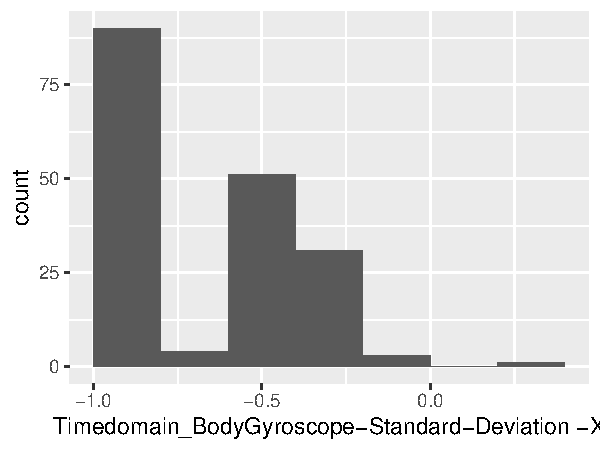
\includegraphics{codebook_tidydatasub_files/figure-latex/Var-24-Timedomain-BodyGyroscope-Standard-Deviation--X-1.pdf}

\end{minipage}

\noindent\makebox[\linewidth]{\rule{\textwidth}{0.4pt}}

\hypertarget{timedomain_bodygyroscope-standard-deviation--y}{%
\subsection{Timedomain\_BodyGyroscope-Standard-Deviation
-Y}\label{timedomain_bodygyroscope-standard-deviation--y}}

\begin{minipage}{0.75 \textwidth}

\begin{longtable}[]{@{}lr@{}}
\toprule
\begin{minipage}[b]{0.34\columnwidth}\raggedright
Feature\strut
\end{minipage} & \begin{minipage}[b]{0.20\columnwidth}\raggedleft
Result\strut
\end{minipage}\tabularnewline
\midrule
\endhead
\begin{minipage}[t]{0.34\columnwidth}\raggedright
Variable type\strut
\end{minipage} & \begin{minipage}[t]{0.20\columnwidth}\raggedleft
numeric\strut
\end{minipage}\tabularnewline
\begin{minipage}[t]{0.34\columnwidth}\raggedright
Number of missing obs.\strut
\end{minipage} & \begin{minipage}[t]{0.20\columnwidth}\raggedleft
0 (0 \%)\strut
\end{minipage}\tabularnewline
\begin{minipage}[t]{0.34\columnwidth}\raggedright
Number of unique values\strut
\end{minipage} & \begin{minipage}[t]{0.20\columnwidth}\raggedleft
180\strut
\end{minipage}\tabularnewline
\begin{minipage}[t]{0.34\columnwidth}\raggedright
Median\strut
\end{minipage} & \begin{minipage}[t]{0.20\columnwidth}\raggedleft
-0.8\strut
\end{minipage}\tabularnewline
\begin{minipage}[t]{0.34\columnwidth}\raggedright
1st and 3rd quartiles\strut
\end{minipage} & \begin{minipage}[t]{0.20\columnwidth}\raggedleft
-0.96; -0.42\strut
\end{minipage}\tabularnewline
\begin{minipage}[t]{0.34\columnwidth}\raggedright
Min. and max.\strut
\end{minipage} & \begin{minipage}[t]{0.20\columnwidth}\raggedleft
-0.99; 0.48\strut
\end{minipage}\tabularnewline
\bottomrule
\end{longtable}

\end{minipage}
\begin{minipage}{0.25 \textwidth}

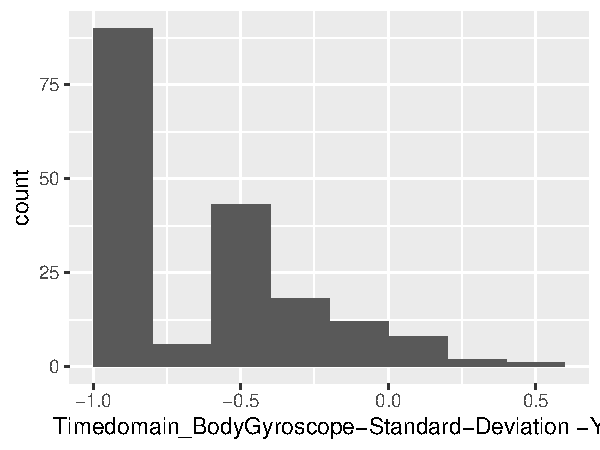
\includegraphics{codebook_tidydatasub_files/figure-latex/Var-25-Timedomain-BodyGyroscope-Standard-Deviation--Y-1.pdf}

\end{minipage}

\noindent\makebox[\linewidth]{\rule{\textwidth}{0.4pt}}

\hypertarget{timedomain_bodygyroscope-standard-deviation--z}{%
\subsection{Timedomain\_BodyGyroscope-Standard-Deviation
-Z}\label{timedomain_bodygyroscope-standard-deviation--z}}

\begin{minipage}{0.75 \textwidth}

\begin{longtable}[]{@{}lr@{}}
\toprule
\begin{minipage}[b]{0.34\columnwidth}\raggedright
Feature\strut
\end{minipage} & \begin{minipage}[b]{0.20\columnwidth}\raggedleft
Result\strut
\end{minipage}\tabularnewline
\midrule
\endhead
\begin{minipage}[t]{0.34\columnwidth}\raggedright
Variable type\strut
\end{minipage} & \begin{minipage}[t]{0.20\columnwidth}\raggedleft
numeric\strut
\end{minipage}\tabularnewline
\begin{minipage}[t]{0.34\columnwidth}\raggedright
Number of missing obs.\strut
\end{minipage} & \begin{minipage}[t]{0.20\columnwidth}\raggedleft
0 (0 \%)\strut
\end{minipage}\tabularnewline
\begin{minipage}[t]{0.34\columnwidth}\raggedright
Number of unique values\strut
\end{minipage} & \begin{minipage}[t]{0.20\columnwidth}\raggedleft
180\strut
\end{minipage}\tabularnewline
\begin{minipage}[t]{0.34\columnwidth}\raggedright
Median\strut
\end{minipage} & \begin{minipage}[t]{0.20\columnwidth}\raggedleft
-0.8\strut
\end{minipage}\tabularnewline
\begin{minipage}[t]{0.34\columnwidth}\raggedright
1st and 3rd quartiles\strut
\end{minipage} & \begin{minipage}[t]{0.20\columnwidth}\raggedleft
-0.96; -0.31\strut
\end{minipage}\tabularnewline
\begin{minipage}[t]{0.34\columnwidth}\raggedright
Min. and max.\strut
\end{minipage} & \begin{minipage}[t]{0.20\columnwidth}\raggedleft
-0.99; 0.56\strut
\end{minipage}\tabularnewline
\bottomrule
\end{longtable}

\end{minipage}
\begin{minipage}{0.25 \textwidth}

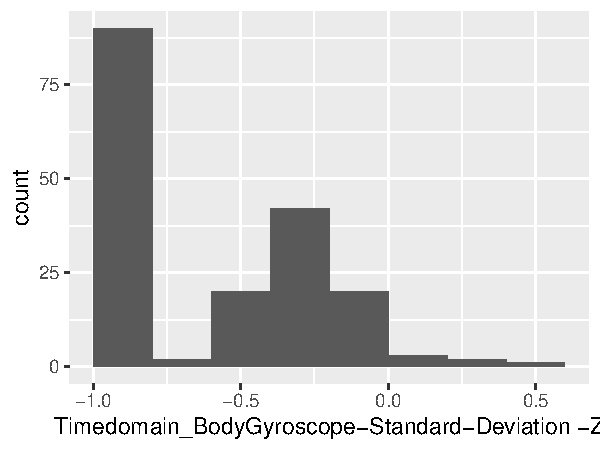
\includegraphics{codebook_tidydatasub_files/figure-latex/Var-26-Timedomain-BodyGyroscope-Standard-Deviation--Z-1.pdf}

\end{minipage}

\noindent\makebox[\linewidth]{\rule{\textwidth}{0.4pt}}

\hypertarget{timedomain_bodygyroscopejerk-mean--x}{%
\subsection{Timedomain\_BodyGyroscopeJerk-mean
-X}\label{timedomain_bodygyroscopejerk-mean--x}}

\begin{minipage}{0.75 \textwidth}

\begin{longtable}[]{@{}lr@{}}
\toprule
\begin{minipage}[b]{0.34\columnwidth}\raggedright
Feature\strut
\end{minipage} & \begin{minipage}[b]{0.20\columnwidth}\raggedleft
Result\strut
\end{minipage}\tabularnewline
\midrule
\endhead
\begin{minipage}[t]{0.34\columnwidth}\raggedright
Variable type\strut
\end{minipage} & \begin{minipage}[t]{0.20\columnwidth}\raggedleft
numeric\strut
\end{minipage}\tabularnewline
\begin{minipage}[t]{0.34\columnwidth}\raggedright
Number of missing obs.\strut
\end{minipage} & \begin{minipage}[t]{0.20\columnwidth}\raggedleft
0 (0 \%)\strut
\end{minipage}\tabularnewline
\begin{minipage}[t]{0.34\columnwidth}\raggedright
Number of unique values\strut
\end{minipage} & \begin{minipage}[t]{0.20\columnwidth}\raggedleft
180\strut
\end{minipage}\tabularnewline
\begin{minipage}[t]{0.34\columnwidth}\raggedright
Median\strut
\end{minipage} & \begin{minipage}[t]{0.20\columnwidth}\raggedleft
-0.1\strut
\end{minipage}\tabularnewline
\begin{minipage}[t]{0.34\columnwidth}\raggedright
1st and 3rd quartiles\strut
\end{minipage} & \begin{minipage}[t]{0.20\columnwidth}\raggedleft
-0.1; -0.09\strut
\end{minipage}\tabularnewline
\begin{minipage}[t]{0.34\columnwidth}\raggedright
Min. and max.\strut
\end{minipage} & \begin{minipage}[t]{0.20\columnwidth}\raggedleft
-0.16; -0.02\strut
\end{minipage}\tabularnewline
\bottomrule
\end{longtable}

\end{minipage}
\begin{minipage}{0.25 \textwidth}

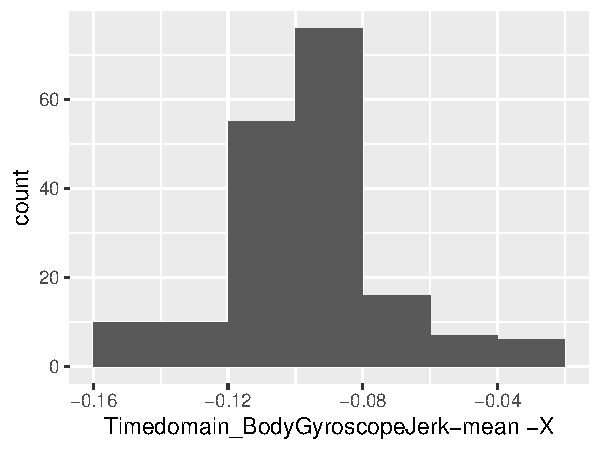
\includegraphics{codebook_tidydatasub_files/figure-latex/Var-27-Timedomain-BodyGyroscopeJerk-mean--X-1.pdf}

\end{minipage}

\noindent\makebox[\linewidth]{\rule{\textwidth}{0.4pt}}

\hypertarget{timedomain_bodygyroscopejerk-mean--y}{%
\subsection{Timedomain\_BodyGyroscopeJerk-mean
-Y}\label{timedomain_bodygyroscopejerk-mean--y}}

\begin{minipage}{0.75 \textwidth}

\begin{longtable}[]{@{}lr@{}}
\toprule
\begin{minipage}[b]{0.34\columnwidth}\raggedright
Feature\strut
\end{minipage} & \begin{minipage}[b]{0.20\columnwidth}\raggedleft
Result\strut
\end{minipage}\tabularnewline
\midrule
\endhead
\begin{minipage}[t]{0.34\columnwidth}\raggedright
Variable type\strut
\end{minipage} & \begin{minipage}[t]{0.20\columnwidth}\raggedleft
numeric\strut
\end{minipage}\tabularnewline
\begin{minipage}[t]{0.34\columnwidth}\raggedright
Number of missing obs.\strut
\end{minipage} & \begin{minipage}[t]{0.20\columnwidth}\raggedleft
0 (0 \%)\strut
\end{minipage}\tabularnewline
\begin{minipage}[t]{0.34\columnwidth}\raggedright
Number of unique values\strut
\end{minipage} & \begin{minipage}[t]{0.20\columnwidth}\raggedleft
180\strut
\end{minipage}\tabularnewline
\begin{minipage}[t]{0.34\columnwidth}\raggedright
Median\strut
\end{minipage} & \begin{minipage}[t]{0.20\columnwidth}\raggedleft
-0.04\strut
\end{minipage}\tabularnewline
\begin{minipage}[t]{0.34\columnwidth}\raggedright
1st and 3rd quartiles\strut
\end{minipage} & \begin{minipage}[t]{0.20\columnwidth}\raggedleft
-0.05; -0.04\strut
\end{minipage}\tabularnewline
\begin{minipage}[t]{0.34\columnwidth}\raggedright
Min. and max.\strut
\end{minipage} & \begin{minipage}[t]{0.20\columnwidth}\raggedleft
-0.08; -0.01\strut
\end{minipage}\tabularnewline
\bottomrule
\end{longtable}

\end{minipage}
\begin{minipage}{0.25 \textwidth}

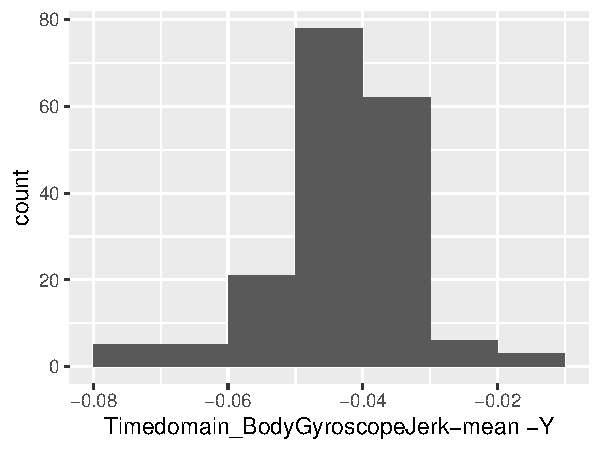
\includegraphics{codebook_tidydatasub_files/figure-latex/Var-28-Timedomain-BodyGyroscopeJerk-mean--Y-1.pdf}

\end{minipage}

\noindent\makebox[\linewidth]{\rule{\textwidth}{0.4pt}}

\hypertarget{timedomain_bodygyroscopejerk-mean--z}{%
\subsection{Timedomain\_BodyGyroscopeJerk-mean
-Z}\label{timedomain_bodygyroscopejerk-mean--z}}

\begin{minipage}{0.75 \textwidth}

\begin{longtable}[]{@{}lr@{}}
\toprule
\begin{minipage}[b]{0.34\columnwidth}\raggedright
Feature\strut
\end{minipage} & \begin{minipage}[b]{0.20\columnwidth}\raggedleft
Result\strut
\end{minipage}\tabularnewline
\midrule
\endhead
\begin{minipage}[t]{0.34\columnwidth}\raggedright
Variable type\strut
\end{minipage} & \begin{minipage}[t]{0.20\columnwidth}\raggedleft
numeric\strut
\end{minipage}\tabularnewline
\begin{minipage}[t]{0.34\columnwidth}\raggedright
Number of missing obs.\strut
\end{minipage} & \begin{minipage}[t]{0.20\columnwidth}\raggedleft
0 (0 \%)\strut
\end{minipage}\tabularnewline
\begin{minipage}[t]{0.34\columnwidth}\raggedright
Number of unique values\strut
\end{minipage} & \begin{minipage}[t]{0.20\columnwidth}\raggedleft
180\strut
\end{minipage}\tabularnewline
\begin{minipage}[t]{0.34\columnwidth}\raggedright
Median\strut
\end{minipage} & \begin{minipage}[t]{0.20\columnwidth}\raggedleft
-0.05\strut
\end{minipage}\tabularnewline
\begin{minipage}[t]{0.34\columnwidth}\raggedright
1st and 3rd quartiles\strut
\end{minipage} & \begin{minipage}[t]{0.20\columnwidth}\raggedleft
-0.06; -0.05\strut
\end{minipage}\tabularnewline
\begin{minipage}[t]{0.34\columnwidth}\raggedright
Min. and max.\strut
\end{minipage} & \begin{minipage}[t]{0.20\columnwidth}\raggedleft
-0.09; -0.01\strut
\end{minipage}\tabularnewline
\bottomrule
\end{longtable}

\end{minipage}
\begin{minipage}{0.25 \textwidth}

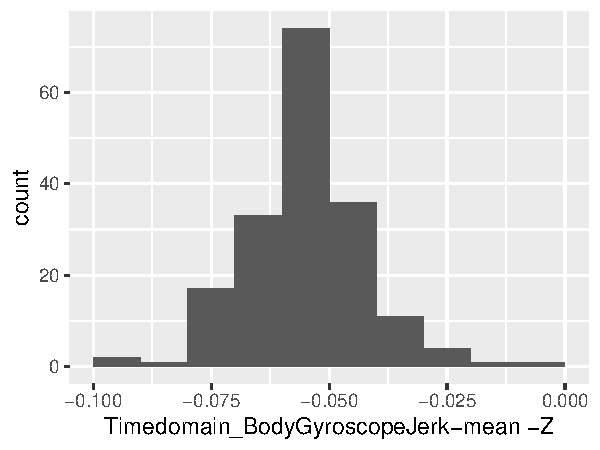
\includegraphics{codebook_tidydatasub_files/figure-latex/Var-29-Timedomain-BodyGyroscopeJerk-mean--Z-1.pdf}

\end{minipage}

\noindent\makebox[\linewidth]{\rule{\textwidth}{0.4pt}}

\hypertarget{timedomain_bodygyroscopejerk-standard-deviation--x}{%
\subsection{Timedomain\_BodyGyroscopeJerk-Standard-Deviation
-X}\label{timedomain_bodygyroscopejerk-standard-deviation--x}}

\begin{minipage}{0.75 \textwidth}

\begin{longtable}[]{@{}lr@{}}
\toprule
\begin{minipage}[b]{0.34\columnwidth}\raggedright
Feature\strut
\end{minipage} & \begin{minipage}[b]{0.20\columnwidth}\raggedleft
Result\strut
\end{minipage}\tabularnewline
\midrule
\endhead
\begin{minipage}[t]{0.34\columnwidth}\raggedright
Variable type\strut
\end{minipage} & \begin{minipage}[t]{0.20\columnwidth}\raggedleft
numeric\strut
\end{minipage}\tabularnewline
\begin{minipage}[t]{0.34\columnwidth}\raggedright
Number of missing obs.\strut
\end{minipage} & \begin{minipage}[t]{0.20\columnwidth}\raggedleft
0 (0 \%)\strut
\end{minipage}\tabularnewline
\begin{minipage}[t]{0.34\columnwidth}\raggedright
Number of unique values\strut
\end{minipage} & \begin{minipage}[t]{0.20\columnwidth}\raggedleft
180\strut
\end{minipage}\tabularnewline
\begin{minipage}[t]{0.34\columnwidth}\raggedright
Median\strut
\end{minipage} & \begin{minipage}[t]{0.20\columnwidth}\raggedleft
-0.84\strut
\end{minipage}\tabularnewline
\begin{minipage}[t]{0.34\columnwidth}\raggedright
1st and 3rd quartiles\strut
\end{minipage} & \begin{minipage}[t]{0.20\columnwidth}\raggedleft
-0.98; -0.46\strut
\end{minipage}\tabularnewline
\begin{minipage}[t]{0.34\columnwidth}\raggedright
Min. and max.\strut
\end{minipage} & \begin{minipage}[t]{0.20\columnwidth}\raggedleft
-1; 0.18\strut
\end{minipage}\tabularnewline
\bottomrule
\end{longtable}

\end{minipage}
\begin{minipage}{0.25 \textwidth}

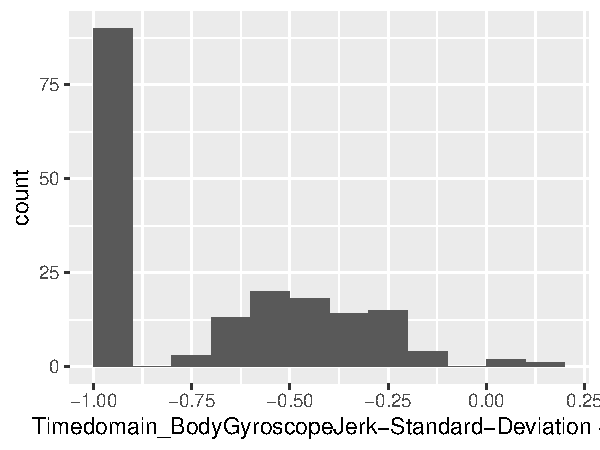
\includegraphics{codebook_tidydatasub_files/figure-latex/Var-30-Timedomain-BodyGyroscopeJerk-Standard-Deviation--X-1.pdf}

\end{minipage}

\noindent\makebox[\linewidth]{\rule{\textwidth}{0.4pt}}

\hypertarget{timedomain_bodygyroscopejerk-standard-deviation--y}{%
\subsection{Timedomain\_BodyGyroscopeJerk-Standard-Deviation
-Y}\label{timedomain_bodygyroscopejerk-standard-deviation--y}}

\begin{minipage}{0.75 \textwidth}

\begin{longtable}[]{@{}lr@{}}
\toprule
\begin{minipage}[b]{0.34\columnwidth}\raggedright
Feature\strut
\end{minipage} & \begin{minipage}[b]{0.20\columnwidth}\raggedleft
Result\strut
\end{minipage}\tabularnewline
\midrule
\endhead
\begin{minipage}[t]{0.34\columnwidth}\raggedright
Variable type\strut
\end{minipage} & \begin{minipage}[t]{0.20\columnwidth}\raggedleft
numeric\strut
\end{minipage}\tabularnewline
\begin{minipage}[t]{0.34\columnwidth}\raggedright
Number of missing obs.\strut
\end{minipage} & \begin{minipage}[t]{0.20\columnwidth}\raggedleft
0 (0 \%)\strut
\end{minipage}\tabularnewline
\begin{minipage}[t]{0.34\columnwidth}\raggedright
Number of unique values\strut
\end{minipage} & \begin{minipage}[t]{0.20\columnwidth}\raggedleft
180\strut
\end{minipage}\tabularnewline
\begin{minipage}[t]{0.34\columnwidth}\raggedright
Median\strut
\end{minipage} & \begin{minipage}[t]{0.20\columnwidth}\raggedleft
-0.89\strut
\end{minipage}\tabularnewline
\begin{minipage}[t]{0.34\columnwidth}\raggedright
1st and 3rd quartiles\strut
\end{minipage} & \begin{minipage}[t]{0.20\columnwidth}\raggedleft
-0.98; -0.59\strut
\end{minipage}\tabularnewline
\begin{minipage}[t]{0.34\columnwidth}\raggedright
Min. and max.\strut
\end{minipage} & \begin{minipage}[t]{0.20\columnwidth}\raggedleft
-1; 0.3\strut
\end{minipage}\tabularnewline
\bottomrule
\end{longtable}

\end{minipage}
\begin{minipage}{0.25 \textwidth}

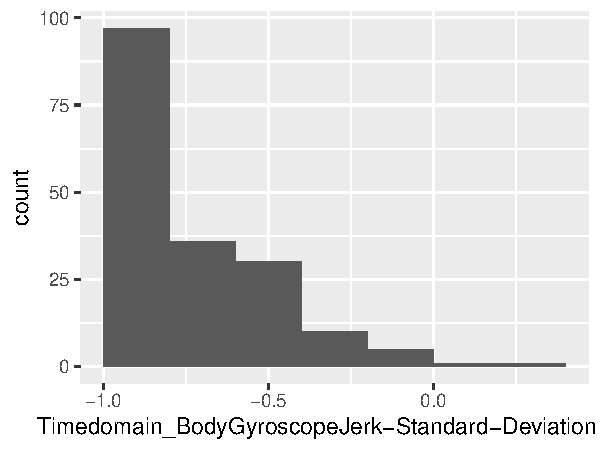
\includegraphics{codebook_tidydatasub_files/figure-latex/Var-31-Timedomain-BodyGyroscopeJerk-Standard-Deviation--Y-1.pdf}

\end{minipage}

\noindent\makebox[\linewidth]{\rule{\textwidth}{0.4pt}}

\hypertarget{timedomain_bodygyroscopejerk-standard-deviation--z}{%
\subsection{Timedomain\_BodyGyroscopeJerk-Standard-Deviation
-Z}\label{timedomain_bodygyroscopejerk-standard-deviation--z}}

\begin{minipage}{0.75 \textwidth}

\begin{longtable}[]{@{}lr@{}}
\toprule
\begin{minipage}[b]{0.34\columnwidth}\raggedright
Feature\strut
\end{minipage} & \begin{minipage}[b]{0.20\columnwidth}\raggedleft
Result\strut
\end{minipage}\tabularnewline
\midrule
\endhead
\begin{minipage}[t]{0.34\columnwidth}\raggedright
Variable type\strut
\end{minipage} & \begin{minipage}[t]{0.20\columnwidth}\raggedleft
numeric\strut
\end{minipage}\tabularnewline
\begin{minipage}[t]{0.34\columnwidth}\raggedright
Number of missing obs.\strut
\end{minipage} & \begin{minipage}[t]{0.20\columnwidth}\raggedleft
0 (0 \%)\strut
\end{minipage}\tabularnewline
\begin{minipage}[t]{0.34\columnwidth}\raggedright
Number of unique values\strut
\end{minipage} & \begin{minipage}[t]{0.20\columnwidth}\raggedleft
180\strut
\end{minipage}\tabularnewline
\begin{minipage}[t]{0.34\columnwidth}\raggedright
Median\strut
\end{minipage} & \begin{minipage}[t]{0.20\columnwidth}\raggedleft
-0.86\strut
\end{minipage}\tabularnewline
\begin{minipage}[t]{0.34\columnwidth}\raggedright
1st and 3rd quartiles\strut
\end{minipage} & \begin{minipage}[t]{0.20\columnwidth}\raggedleft
-0.98; -0.47\strut
\end{minipage}\tabularnewline
\begin{minipage}[t]{0.34\columnwidth}\raggedright
Min. and max.\strut
\end{minipage} & \begin{minipage}[t]{0.20\columnwidth}\raggedleft
-1; 0.19\strut
\end{minipage}\tabularnewline
\bottomrule
\end{longtable}

\end{minipage}
\begin{minipage}{0.25 \textwidth}

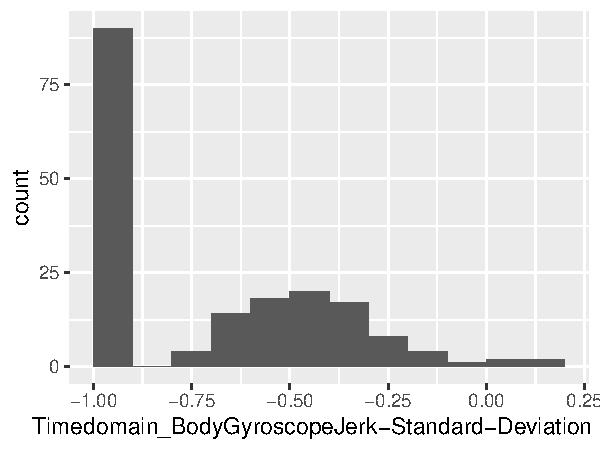
\includegraphics{codebook_tidydatasub_files/figure-latex/Var-32-Timedomain-BodyGyroscopeJerk-Standard-Deviation--Z-1.pdf}

\end{minipage}

\noindent\makebox[\linewidth]{\rule{\textwidth}{0.4pt}}

\hypertarget{timedomain_bodyacceleration_mag-mean}{%
\subsection{Timedomain\_BodyAcceleration\_Mag-mean}\label{timedomain_bodyacceleration_mag-mean}}

\begin{minipage}{0.75 \textwidth}

\begin{longtable}[]{@{}lr@{}}
\toprule
\begin{minipage}[b]{0.34\columnwidth}\raggedright
Feature\strut
\end{minipage} & \begin{minipage}[b]{0.20\columnwidth}\raggedleft
Result\strut
\end{minipage}\tabularnewline
\midrule
\endhead
\begin{minipage}[t]{0.34\columnwidth}\raggedright
Variable type\strut
\end{minipage} & \begin{minipage}[t]{0.20\columnwidth}\raggedleft
numeric\strut
\end{minipage}\tabularnewline
\begin{minipage}[t]{0.34\columnwidth}\raggedright
Number of missing obs.\strut
\end{minipage} & \begin{minipage}[t]{0.20\columnwidth}\raggedleft
0 (0 \%)\strut
\end{minipage}\tabularnewline
\begin{minipage}[t]{0.34\columnwidth}\raggedright
Number of unique values\strut
\end{minipage} & \begin{minipage}[t]{0.20\columnwidth}\raggedleft
180\strut
\end{minipage}\tabularnewline
\begin{minipage}[t]{0.34\columnwidth}\raggedright
Median\strut
\end{minipage} & \begin{minipage}[t]{0.20\columnwidth}\raggedleft
-0.48\strut
\end{minipage}\tabularnewline
\begin{minipage}[t]{0.34\columnwidth}\raggedright
1st and 3rd quartiles\strut
\end{minipage} & \begin{minipage}[t]{0.20\columnwidth}\raggedleft
-0.96; -0.09\strut
\end{minipage}\tabularnewline
\begin{minipage}[t]{0.34\columnwidth}\raggedright
Min. and max.\strut
\end{minipage} & \begin{minipage}[t]{0.20\columnwidth}\raggedleft
-0.99; 0.64\strut
\end{minipage}\tabularnewline
\bottomrule
\end{longtable}

\end{minipage}
\begin{minipage}{0.25 \textwidth}

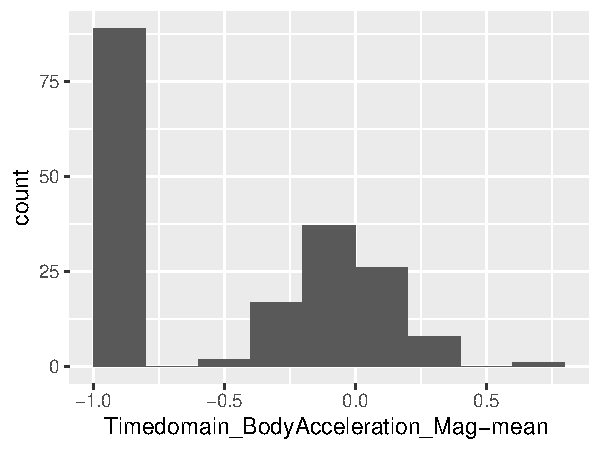
\includegraphics{codebook_tidydatasub_files/figure-latex/Var-33-Timedomain-BodyAcceleration-Mag-mean--1.pdf}

\end{minipage}

\noindent\makebox[\linewidth]{\rule{\textwidth}{0.4pt}}

\hypertarget{timedomain_bodyacceleration_mag-standard-deviation}{%
\subsection{Timedomain\_BodyAcceleration\_Mag-Standard-Deviation}\label{timedomain_bodyacceleration_mag-standard-deviation}}

\begin{minipage}{0.75 \textwidth}

\begin{longtable}[]{@{}lr@{}}
\toprule
\begin{minipage}[b]{0.34\columnwidth}\raggedright
Feature\strut
\end{minipage} & \begin{minipage}[b]{0.20\columnwidth}\raggedleft
Result\strut
\end{minipage}\tabularnewline
\midrule
\endhead
\begin{minipage}[t]{0.34\columnwidth}\raggedright
Variable type\strut
\end{minipage} & \begin{minipage}[t]{0.20\columnwidth}\raggedleft
numeric\strut
\end{minipage}\tabularnewline
\begin{minipage}[t]{0.34\columnwidth}\raggedright
Number of missing obs.\strut
\end{minipage} & \begin{minipage}[t]{0.20\columnwidth}\raggedleft
0 (0 \%)\strut
\end{minipage}\tabularnewline
\begin{minipage}[t]{0.34\columnwidth}\raggedright
Number of unique values\strut
\end{minipage} & \begin{minipage}[t]{0.20\columnwidth}\raggedleft
180\strut
\end{minipage}\tabularnewline
\begin{minipage}[t]{0.34\columnwidth}\raggedright
Median\strut
\end{minipage} & \begin{minipage}[t]{0.20\columnwidth}\raggedleft
-0.61\strut
\end{minipage}\tabularnewline
\begin{minipage}[t]{0.34\columnwidth}\raggedright
1st and 3rd quartiles\strut
\end{minipage} & \begin{minipage}[t]{0.20\columnwidth}\raggedleft
-0.94; -0.21\strut
\end{minipage}\tabularnewline
\begin{minipage}[t]{0.34\columnwidth}\raggedright
Min. and max.\strut
\end{minipage} & \begin{minipage}[t]{0.20\columnwidth}\raggedleft
-0.99; 0.43\strut
\end{minipage}\tabularnewline
\bottomrule
\end{longtable}

\end{minipage}
\begin{minipage}{0.25 \textwidth}

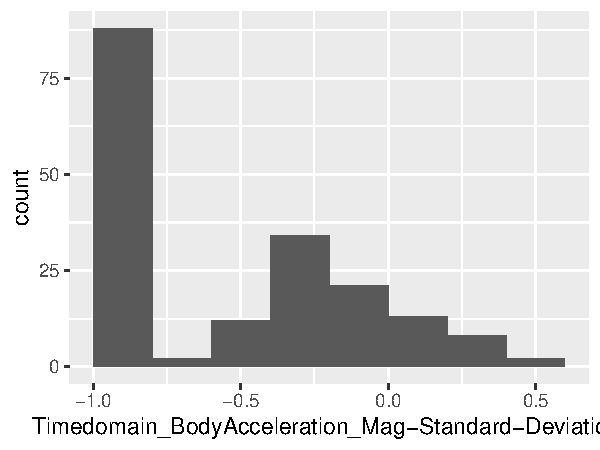
\includegraphics{codebook_tidydatasub_files/figure-latex/Var-34-Timedomain-BodyAcceleration-Mag-Standard-Deviation--1.pdf}

\end{minipage}

\noindent\makebox[\linewidth]{\rule{\textwidth}{0.4pt}}

\hypertarget{timedomain_gravityacceleration_mag-mean}{%
\subsection{Timedomain\_GravityAcceleration\_Mag-mean}\label{timedomain_gravityacceleration_mag-mean}}

\begin{minipage}{0.75 \textwidth}

\begin{longtable}[]{@{}lr@{}}
\toprule
\begin{minipage}[b]{0.34\columnwidth}\raggedright
Feature\strut
\end{minipage} & \begin{minipage}[b]{0.20\columnwidth}\raggedleft
Result\strut
\end{minipage}\tabularnewline
\midrule
\endhead
\begin{minipage}[t]{0.34\columnwidth}\raggedright
Variable type\strut
\end{minipage} & \begin{minipage}[t]{0.20\columnwidth}\raggedleft
numeric\strut
\end{minipage}\tabularnewline
\begin{minipage}[t]{0.34\columnwidth}\raggedright
Number of missing obs.\strut
\end{minipage} & \begin{minipage}[t]{0.20\columnwidth}\raggedleft
0 (0 \%)\strut
\end{minipage}\tabularnewline
\begin{minipage}[t]{0.34\columnwidth}\raggedright
Number of unique values\strut
\end{minipage} & \begin{minipage}[t]{0.20\columnwidth}\raggedleft
180\strut
\end{minipage}\tabularnewline
\begin{minipage}[t]{0.34\columnwidth}\raggedright
Median\strut
\end{minipage} & \begin{minipage}[t]{0.20\columnwidth}\raggedleft
-0.48\strut
\end{minipage}\tabularnewline
\begin{minipage}[t]{0.34\columnwidth}\raggedright
1st and 3rd quartiles\strut
\end{minipage} & \begin{minipage}[t]{0.20\columnwidth}\raggedleft
-0.96; -0.09\strut
\end{minipage}\tabularnewline
\begin{minipage}[t]{0.34\columnwidth}\raggedright
Min. and max.\strut
\end{minipage} & \begin{minipage}[t]{0.20\columnwidth}\raggedleft
-0.99; 0.64\strut
\end{minipage}\tabularnewline
\bottomrule
\end{longtable}

\end{minipage}
\begin{minipage}{0.25 \textwidth}

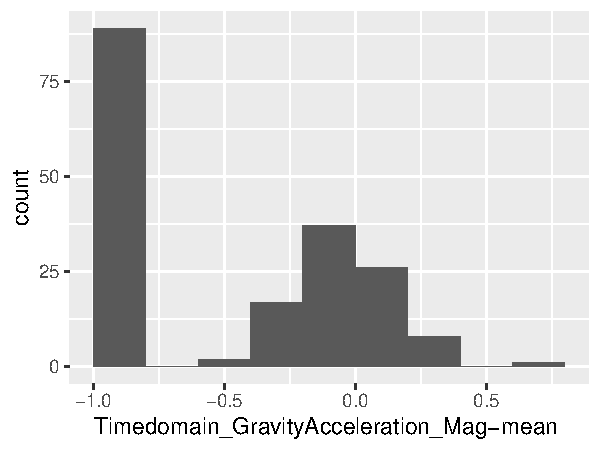
\includegraphics{codebook_tidydatasub_files/figure-latex/Var-35-Timedomain-GravityAcceleration-Mag-mean--1.pdf}

\end{minipage}

\noindent\makebox[\linewidth]{\rule{\textwidth}{0.4pt}}

\hypertarget{timedomain_gravityacceleration_mag-standard-deviation}{%
\subsection{Timedomain\_GravityAcceleration\_Mag-Standard-Deviation}\label{timedomain_gravityacceleration_mag-standard-deviation}}

\begin{minipage}{0.75 \textwidth}

\begin{longtable}[]{@{}lr@{}}
\toprule
\begin{minipage}[b]{0.34\columnwidth}\raggedright
Feature\strut
\end{minipage} & \begin{minipage}[b]{0.20\columnwidth}\raggedleft
Result\strut
\end{minipage}\tabularnewline
\midrule
\endhead
\begin{minipage}[t]{0.34\columnwidth}\raggedright
Variable type\strut
\end{minipage} & \begin{minipage}[t]{0.20\columnwidth}\raggedleft
numeric\strut
\end{minipage}\tabularnewline
\begin{minipage}[t]{0.34\columnwidth}\raggedright
Number of missing obs.\strut
\end{minipage} & \begin{minipage}[t]{0.20\columnwidth}\raggedleft
0 (0 \%)\strut
\end{minipage}\tabularnewline
\begin{minipage}[t]{0.34\columnwidth}\raggedright
Number of unique values\strut
\end{minipage} & \begin{minipage}[t]{0.20\columnwidth}\raggedleft
180\strut
\end{minipage}\tabularnewline
\begin{minipage}[t]{0.34\columnwidth}\raggedright
Median\strut
\end{minipage} & \begin{minipage}[t]{0.20\columnwidth}\raggedleft
-0.61\strut
\end{minipage}\tabularnewline
\begin{minipage}[t]{0.34\columnwidth}\raggedright
1st and 3rd quartiles\strut
\end{minipage} & \begin{minipage}[t]{0.20\columnwidth}\raggedleft
-0.94; -0.21\strut
\end{minipage}\tabularnewline
\begin{minipage}[t]{0.34\columnwidth}\raggedright
Min. and max.\strut
\end{minipage} & \begin{minipage}[t]{0.20\columnwidth}\raggedleft
-0.99; 0.43\strut
\end{minipage}\tabularnewline
\bottomrule
\end{longtable}

\end{minipage}
\begin{minipage}{0.25 \textwidth}

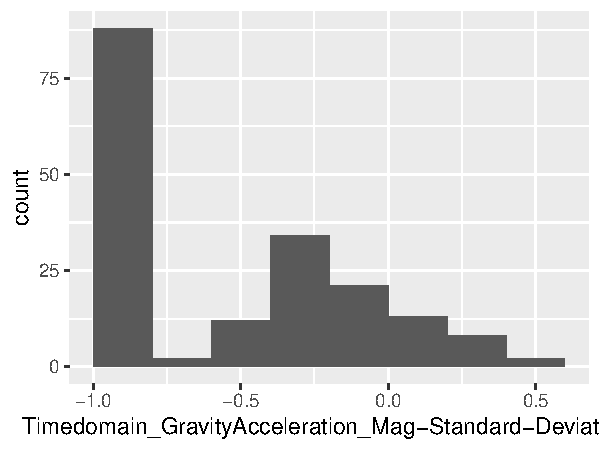
\includegraphics{codebook_tidydatasub_files/figure-latex/Var-36-Timedomain-GravityAcceleration-Mag-Standard-Deviation--1.pdf}

\end{minipage}

\noindent\makebox[\linewidth]{\rule{\textwidth}{0.4pt}}

\hypertarget{timedomain_bodyacceleration_jerkmag-mean}{%
\subsection{Timedomain\_BodyAcceleration\_JerkMag-mean}\label{timedomain_bodyacceleration_jerkmag-mean}}

\begin{minipage}{0.75 \textwidth}

\begin{longtable}[]{@{}lr@{}}
\toprule
\begin{minipage}[b]{0.34\columnwidth}\raggedright
Feature\strut
\end{minipage} & \begin{minipage}[b]{0.20\columnwidth}\raggedleft
Result\strut
\end{minipage}\tabularnewline
\midrule
\endhead
\begin{minipage}[t]{0.34\columnwidth}\raggedright
Variable type\strut
\end{minipage} & \begin{minipage}[t]{0.20\columnwidth}\raggedleft
numeric\strut
\end{minipage}\tabularnewline
\begin{minipage}[t]{0.34\columnwidth}\raggedright
Number of missing obs.\strut
\end{minipage} & \begin{minipage}[t]{0.20\columnwidth}\raggedleft
0 (0 \%)\strut
\end{minipage}\tabularnewline
\begin{minipage}[t]{0.34\columnwidth}\raggedright
Number of unique values\strut
\end{minipage} & \begin{minipage}[t]{0.20\columnwidth}\raggedleft
180\strut
\end{minipage}\tabularnewline
\begin{minipage}[t]{0.34\columnwidth}\raggedright
Median\strut
\end{minipage} & \begin{minipage}[t]{0.20\columnwidth}\raggedleft
-0.82\strut
\end{minipage}\tabularnewline
\begin{minipage}[t]{0.34\columnwidth}\raggedright
1st and 3rd quartiles\strut
\end{minipage} & \begin{minipage}[t]{0.20\columnwidth}\raggedleft
-0.98; -0.25\strut
\end{minipage}\tabularnewline
\begin{minipage}[t]{0.34\columnwidth}\raggedright
Min. and max.\strut
\end{minipage} & \begin{minipage}[t]{0.20\columnwidth}\raggedleft
-0.99; 0.43\strut
\end{minipage}\tabularnewline
\bottomrule
\end{longtable}

\end{minipage}
\begin{minipage}{0.25 \textwidth}

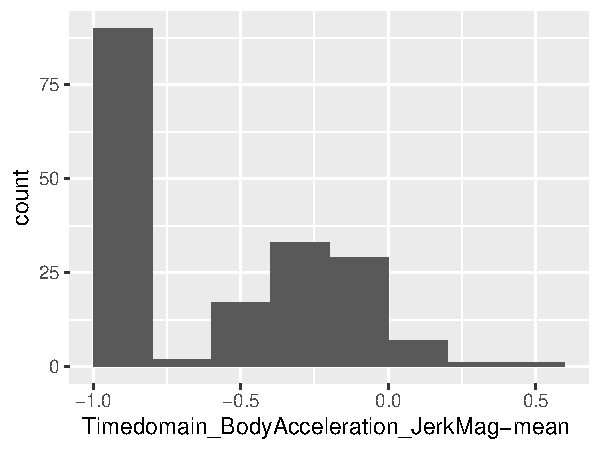
\includegraphics{codebook_tidydatasub_files/figure-latex/Var-37-Timedomain-BodyAcceleration-JerkMag-mean--1.pdf}

\end{minipage}

\noindent\makebox[\linewidth]{\rule{\textwidth}{0.4pt}}

\hypertarget{timedomain_bodyacceleration_jerkmag-standard-deviation}{%
\subsection{Timedomain\_BodyAcceleration\_JerkMag-Standard-Deviation}\label{timedomain_bodyacceleration_jerkmag-standard-deviation}}

\begin{minipage}{0.75 \textwidth}

\begin{longtable}[]{@{}lr@{}}
\toprule
\begin{minipage}[b]{0.34\columnwidth}\raggedright
Feature\strut
\end{minipage} & \begin{minipage}[b]{0.20\columnwidth}\raggedleft
Result\strut
\end{minipage}\tabularnewline
\midrule
\endhead
\begin{minipage}[t]{0.34\columnwidth}\raggedright
Variable type\strut
\end{minipage} & \begin{minipage}[t]{0.20\columnwidth}\raggedleft
numeric\strut
\end{minipage}\tabularnewline
\begin{minipage}[t]{0.34\columnwidth}\raggedright
Number of missing obs.\strut
\end{minipage} & \begin{minipage}[t]{0.20\columnwidth}\raggedleft
0 (0 \%)\strut
\end{minipage}\tabularnewline
\begin{minipage}[t]{0.34\columnwidth}\raggedright
Number of unique values\strut
\end{minipage} & \begin{minipage}[t]{0.20\columnwidth}\raggedleft
180\strut
\end{minipage}\tabularnewline
\begin{minipage}[t]{0.34\columnwidth}\raggedright
Median\strut
\end{minipage} & \begin{minipage}[t]{0.20\columnwidth}\raggedleft
-0.8\strut
\end{minipage}\tabularnewline
\begin{minipage}[t]{0.34\columnwidth}\raggedright
1st and 3rd quartiles\strut
\end{minipage} & \begin{minipage}[t]{0.20\columnwidth}\raggedleft
-0.98; -0.22\strut
\end{minipage}\tabularnewline
\begin{minipage}[t]{0.34\columnwidth}\raggedright
Min. and max.\strut
\end{minipage} & \begin{minipage}[t]{0.20\columnwidth}\raggedleft
-0.99; 0.45\strut
\end{minipage}\tabularnewline
\bottomrule
\end{longtable}

\end{minipage}
\begin{minipage}{0.25 \textwidth}

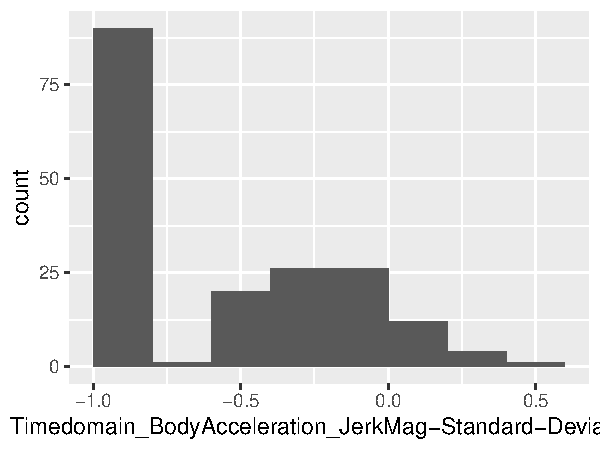
\includegraphics{codebook_tidydatasub_files/figure-latex/Var-38-Timedomain-BodyAcceleration-JerkMag-Standard-Deviation--1.pdf}

\end{minipage}

\noindent\makebox[\linewidth]{\rule{\textwidth}{0.4pt}}

\hypertarget{timedomain_bodygyroscopemag-mean}{%
\subsection{Timedomain\_BodyGyroscopeMag-mean}\label{timedomain_bodygyroscopemag-mean}}

\begin{minipage}{0.75 \textwidth}

\begin{longtable}[]{@{}lr@{}}
\toprule
\begin{minipage}[b]{0.34\columnwidth}\raggedright
Feature\strut
\end{minipage} & \begin{minipage}[b]{0.20\columnwidth}\raggedleft
Result\strut
\end{minipage}\tabularnewline
\midrule
\endhead
\begin{minipage}[t]{0.34\columnwidth}\raggedright
Variable type\strut
\end{minipage} & \begin{minipage}[t]{0.20\columnwidth}\raggedleft
numeric\strut
\end{minipage}\tabularnewline
\begin{minipage}[t]{0.34\columnwidth}\raggedright
Number of missing obs.\strut
\end{minipage} & \begin{minipage}[t]{0.20\columnwidth}\raggedleft
0 (0 \%)\strut
\end{minipage}\tabularnewline
\begin{minipage}[t]{0.34\columnwidth}\raggedright
Number of unique values\strut
\end{minipage} & \begin{minipage}[t]{0.20\columnwidth}\raggedleft
180\strut
\end{minipage}\tabularnewline
\begin{minipage}[t]{0.34\columnwidth}\raggedright
Median\strut
\end{minipage} & \begin{minipage}[t]{0.20\columnwidth}\raggedleft
-0.66\strut
\end{minipage}\tabularnewline
\begin{minipage}[t]{0.34\columnwidth}\raggedright
1st and 3rd quartiles\strut
\end{minipage} & \begin{minipage}[t]{0.20\columnwidth}\raggedleft
-0.95; -0.22\strut
\end{minipage}\tabularnewline
\begin{minipage}[t]{0.34\columnwidth}\raggedright
Min. and max.\strut
\end{minipage} & \begin{minipage}[t]{0.20\columnwidth}\raggedleft
-0.98; 0.42\strut
\end{minipage}\tabularnewline
\bottomrule
\end{longtable}

\end{minipage}
\begin{minipage}{0.25 \textwidth}

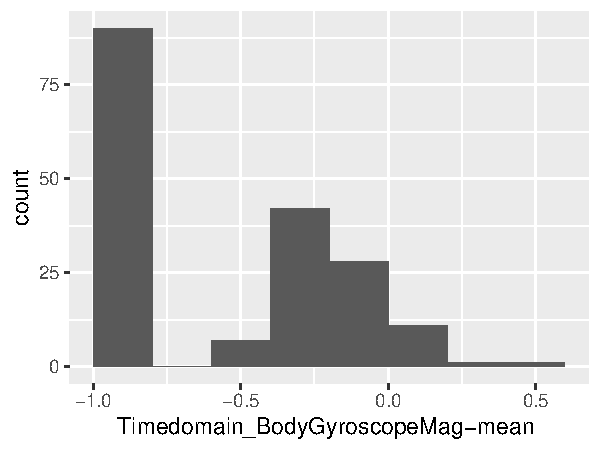
\includegraphics{codebook_tidydatasub_files/figure-latex/Var-39-Timedomain-BodyGyroscopeMag-mean--1.pdf}

\end{minipage}

\noindent\makebox[\linewidth]{\rule{\textwidth}{0.4pt}}

\hypertarget{timedomain_bodygyroscopemag-standard-deviation}{%
\subsection{Timedomain\_BodyGyroscopeMag-Standard-Deviation}\label{timedomain_bodygyroscopemag-standard-deviation}}

\begin{minipage}{0.75 \textwidth}

\begin{longtable}[]{@{}lr@{}}
\toprule
\begin{minipage}[b]{0.34\columnwidth}\raggedright
Feature\strut
\end{minipage} & \begin{minipage}[b]{0.20\columnwidth}\raggedleft
Result\strut
\end{minipage}\tabularnewline
\midrule
\endhead
\begin{minipage}[t]{0.34\columnwidth}\raggedright
Variable type\strut
\end{minipage} & \begin{minipage}[t]{0.20\columnwidth}\raggedleft
numeric\strut
\end{minipage}\tabularnewline
\begin{minipage}[t]{0.34\columnwidth}\raggedright
Number of missing obs.\strut
\end{minipage} & \begin{minipage}[t]{0.20\columnwidth}\raggedleft
0 (0 \%)\strut
\end{minipage}\tabularnewline
\begin{minipage}[t]{0.34\columnwidth}\raggedright
Number of unique values\strut
\end{minipage} & \begin{minipage}[t]{0.20\columnwidth}\raggedleft
180\strut
\end{minipage}\tabularnewline
\begin{minipage}[t]{0.34\columnwidth}\raggedright
Median\strut
\end{minipage} & \begin{minipage}[t]{0.20\columnwidth}\raggedleft
-0.74\strut
\end{minipage}\tabularnewline
\begin{minipage}[t]{0.34\columnwidth}\raggedright
1st and 3rd quartiles\strut
\end{minipage} & \begin{minipage}[t]{0.20\columnwidth}\raggedleft
-0.95; -0.36\strut
\end{minipage}\tabularnewline
\begin{minipage}[t]{0.34\columnwidth}\raggedright
Min. and max.\strut
\end{minipage} & \begin{minipage}[t]{0.20\columnwidth}\raggedleft
-0.98; 0.3\strut
\end{minipage}\tabularnewline
\bottomrule
\end{longtable}

\end{minipage}
\begin{minipage}{0.25 \textwidth}

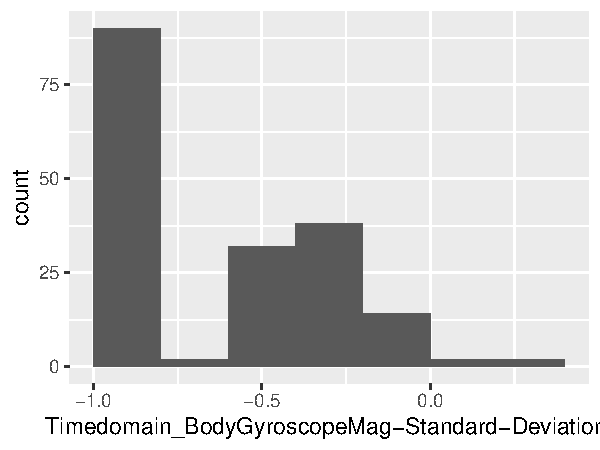
\includegraphics{codebook_tidydatasub_files/figure-latex/Var-40-Timedomain-BodyGyroscopeMag-Standard-Deviation--1.pdf}

\end{minipage}

\noindent\makebox[\linewidth]{\rule{\textwidth}{0.4pt}}

\hypertarget{timedomain_bodygyroscopejerkmag-mean}{%
\subsection{Timedomain\_BodyGyroscopeJerkMag-mean}\label{timedomain_bodygyroscopejerkmag-mean}}

\begin{minipage}{0.75 \textwidth}

\begin{longtable}[]{@{}lr@{}}
\toprule
\begin{minipage}[b]{0.34\columnwidth}\raggedright
Feature\strut
\end{minipage} & \begin{minipage}[b]{0.20\columnwidth}\raggedleft
Result\strut
\end{minipage}\tabularnewline
\midrule
\endhead
\begin{minipage}[t]{0.34\columnwidth}\raggedright
Variable type\strut
\end{minipage} & \begin{minipage}[t]{0.20\columnwidth}\raggedleft
numeric\strut
\end{minipage}\tabularnewline
\begin{minipage}[t]{0.34\columnwidth}\raggedright
Number of missing obs.\strut
\end{minipage} & \begin{minipage}[t]{0.20\columnwidth}\raggedleft
0 (0 \%)\strut
\end{minipage}\tabularnewline
\begin{minipage}[t]{0.34\columnwidth}\raggedright
Number of unique values\strut
\end{minipage} & \begin{minipage}[t]{0.20\columnwidth}\raggedleft
180\strut
\end{minipage}\tabularnewline
\begin{minipage}[t]{0.34\columnwidth}\raggedright
Median\strut
\end{minipage} & \begin{minipage}[t]{0.20\columnwidth}\raggedleft
-0.86\strut
\end{minipage}\tabularnewline
\begin{minipage}[t]{0.34\columnwidth}\raggedright
1st and 3rd quartiles\strut
\end{minipage} & \begin{minipage}[t]{0.20\columnwidth}\raggedleft
-0.99; -0.51\strut
\end{minipage}\tabularnewline
\begin{minipage}[t]{0.34\columnwidth}\raggedright
Min. and max.\strut
\end{minipage} & \begin{minipage}[t]{0.20\columnwidth}\raggedleft
-1; 0.09\strut
\end{minipage}\tabularnewline
\bottomrule
\end{longtable}

\end{minipage}
\begin{minipage}{0.25 \textwidth}

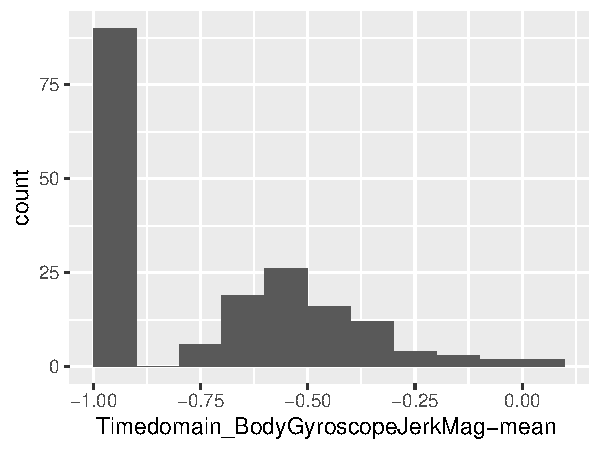
\includegraphics{codebook_tidydatasub_files/figure-latex/Var-41-Timedomain-BodyGyroscopeJerkMag-mean--1.pdf}

\end{minipage}

\noindent\makebox[\linewidth]{\rule{\textwidth}{0.4pt}}

\hypertarget{timedomain_bodygyroscopejerkmag-standard-deviation}{%
\subsection{Timedomain\_BodyGyroscopeJerkMag-Standard-Deviation}\label{timedomain_bodygyroscopejerkmag-standard-deviation}}

\begin{minipage}{0.75 \textwidth}

\begin{longtable}[]{@{}lr@{}}
\toprule
\begin{minipage}[b]{0.34\columnwidth}\raggedright
Feature\strut
\end{minipage} & \begin{minipage}[b]{0.20\columnwidth}\raggedleft
Result\strut
\end{minipage}\tabularnewline
\midrule
\endhead
\begin{minipage}[t]{0.34\columnwidth}\raggedright
Variable type\strut
\end{minipage} & \begin{minipage}[t]{0.20\columnwidth}\raggedleft
numeric\strut
\end{minipage}\tabularnewline
\begin{minipage}[t]{0.34\columnwidth}\raggedright
Number of missing obs.\strut
\end{minipage} & \begin{minipage}[t]{0.20\columnwidth}\raggedleft
0 (0 \%)\strut
\end{minipage}\tabularnewline
\begin{minipage}[t]{0.34\columnwidth}\raggedright
Number of unique values\strut
\end{minipage} & \begin{minipage}[t]{0.20\columnwidth}\raggedleft
180\strut
\end{minipage}\tabularnewline
\begin{minipage}[t]{0.34\columnwidth}\raggedright
Median\strut
\end{minipage} & \begin{minipage}[t]{0.20\columnwidth}\raggedleft
-0.88\strut
\end{minipage}\tabularnewline
\begin{minipage}[t]{0.34\columnwidth}\raggedright
1st and 3rd quartiles\strut
\end{minipage} & \begin{minipage}[t]{0.20\columnwidth}\raggedleft
-0.98; -0.58\strut
\end{minipage}\tabularnewline
\begin{minipage}[t]{0.34\columnwidth}\raggedright
Min. and max.\strut
\end{minipage} & \begin{minipage}[t]{0.20\columnwidth}\raggedleft
-1; 0.25\strut
\end{minipage}\tabularnewline
\bottomrule
\end{longtable}

\end{minipage}
\begin{minipage}{0.25 \textwidth}

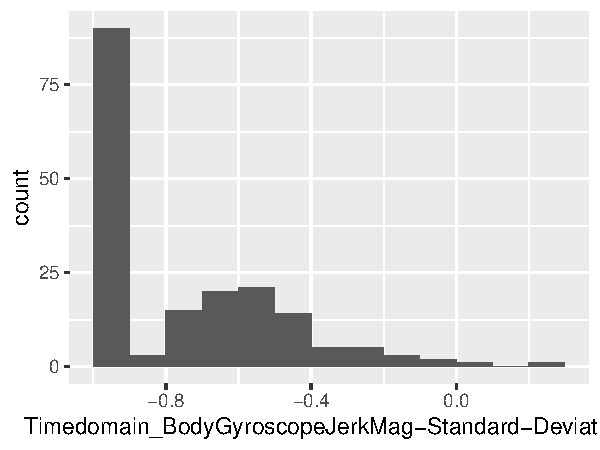
\includegraphics{codebook_tidydatasub_files/figure-latex/Var-42-Timedomain-BodyGyroscopeJerkMag-Standard-Deviation--1.pdf}

\end{minipage}

\noindent\makebox[\linewidth]{\rule{\textwidth}{0.4pt}}

\hypertarget{frequency_bodyacceleration_-mean--x}{%
\subsection{Frequency\_BodyAcceleration\_-mean
-X}\label{frequency_bodyacceleration_-mean--x}}

\begin{minipage}{0.75 \textwidth}

\begin{longtable}[]{@{}lr@{}}
\toprule
\begin{minipage}[b]{0.34\columnwidth}\raggedright
Feature\strut
\end{minipage} & \begin{minipage}[b]{0.20\columnwidth}\raggedleft
Result\strut
\end{minipage}\tabularnewline
\midrule
\endhead
\begin{minipage}[t]{0.34\columnwidth}\raggedright
Variable type\strut
\end{minipage} & \begin{minipage}[t]{0.20\columnwidth}\raggedleft
numeric\strut
\end{minipage}\tabularnewline
\begin{minipage}[t]{0.34\columnwidth}\raggedright
Number of missing obs.\strut
\end{minipage} & \begin{minipage}[t]{0.20\columnwidth}\raggedleft
0 (0 \%)\strut
\end{minipage}\tabularnewline
\begin{minipage}[t]{0.34\columnwidth}\raggedright
Number of unique values\strut
\end{minipage} & \begin{minipage}[t]{0.20\columnwidth}\raggedleft
180\strut
\end{minipage}\tabularnewline
\begin{minipage}[t]{0.34\columnwidth}\raggedright
Median\strut
\end{minipage} & \begin{minipage}[t]{0.20\columnwidth}\raggedleft
-0.77\strut
\end{minipage}\tabularnewline
\begin{minipage}[t]{0.34\columnwidth}\raggedright
1st and 3rd quartiles\strut
\end{minipage} & \begin{minipage}[t]{0.20\columnwidth}\raggedleft
-0.98; -0.22\strut
\end{minipage}\tabularnewline
\begin{minipage}[t]{0.34\columnwidth}\raggedright
Min. and max.\strut
\end{minipage} & \begin{minipage}[t]{0.20\columnwidth}\raggedleft
-1; 0.54\strut
\end{minipage}\tabularnewline
\bottomrule
\end{longtable}

\end{minipage}
\begin{minipage}{0.25 \textwidth}

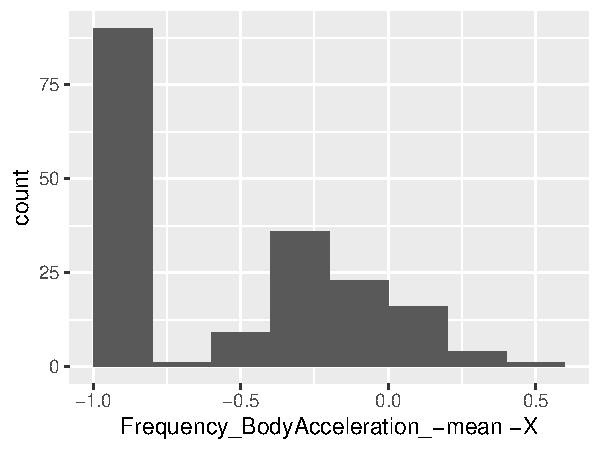
\includegraphics{codebook_tidydatasub_files/figure-latex/Var-43-Frequency-BodyAcceleration--mean--X-1.pdf}

\end{minipage}

\noindent\makebox[\linewidth]{\rule{\textwidth}{0.4pt}}

\hypertarget{frequency_bodyacceleration_-mean--y}{%
\subsection{Frequency\_BodyAcceleration\_-mean
-Y}\label{frequency_bodyacceleration_-mean--y}}

\begin{minipage}{0.75 \textwidth}

\begin{longtable}[]{@{}lr@{}}
\toprule
\begin{minipage}[b]{0.34\columnwidth}\raggedright
Feature\strut
\end{minipage} & \begin{minipage}[b]{0.20\columnwidth}\raggedleft
Result\strut
\end{minipage}\tabularnewline
\midrule
\endhead
\begin{minipage}[t]{0.34\columnwidth}\raggedright
Variable type\strut
\end{minipage} & \begin{minipage}[t]{0.20\columnwidth}\raggedleft
numeric\strut
\end{minipage}\tabularnewline
\begin{minipage}[t]{0.34\columnwidth}\raggedright
Number of missing obs.\strut
\end{minipage} & \begin{minipage}[t]{0.20\columnwidth}\raggedleft
0 (0 \%)\strut
\end{minipage}\tabularnewline
\begin{minipage}[t]{0.34\columnwidth}\raggedright
Number of unique values\strut
\end{minipage} & \begin{minipage}[t]{0.20\columnwidth}\raggedleft
180\strut
\end{minipage}\tabularnewline
\begin{minipage}[t]{0.34\columnwidth}\raggedright
Median\strut
\end{minipage} & \begin{minipage}[t]{0.20\columnwidth}\raggedleft
-0.59\strut
\end{minipage}\tabularnewline
\begin{minipage}[t]{0.34\columnwidth}\raggedright
1st and 3rd quartiles\strut
\end{minipage} & \begin{minipage}[t]{0.20\columnwidth}\raggedleft
-0.95; -0.06\strut
\end{minipage}\tabularnewline
\begin{minipage}[t]{0.34\columnwidth}\raggedright
Min. and max.\strut
\end{minipage} & \begin{minipage}[t]{0.20\columnwidth}\raggedleft
-0.99; 0.52\strut
\end{minipage}\tabularnewline
\bottomrule
\end{longtable}

\end{minipage}
\begin{minipage}{0.25 \textwidth}

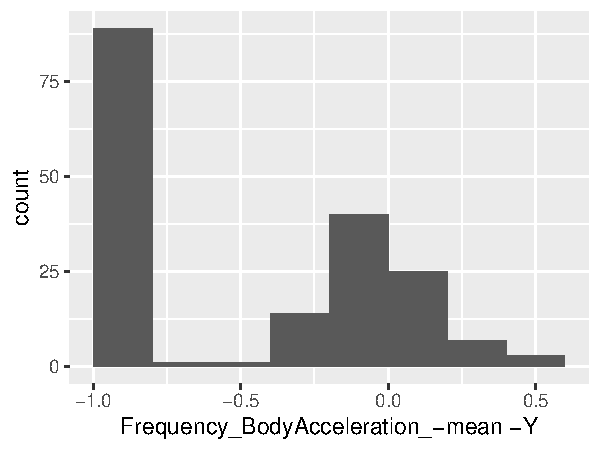
\includegraphics{codebook_tidydatasub_files/figure-latex/Var-44-Frequency-BodyAcceleration--mean--Y-1.pdf}

\end{minipage}

\noindent\makebox[\linewidth]{\rule{\textwidth}{0.4pt}}

\hypertarget{frequency_bodyacceleration_-mean--z}{%
\subsection{Frequency\_BodyAcceleration\_-mean
-Z}\label{frequency_bodyacceleration_-mean--z}}

\begin{minipage}{0.75 \textwidth}

\begin{longtable}[]{@{}lr@{}}
\toprule
\begin{minipage}[b]{0.34\columnwidth}\raggedright
Feature\strut
\end{minipage} & \begin{minipage}[b]{0.20\columnwidth}\raggedleft
Result\strut
\end{minipage}\tabularnewline
\midrule
\endhead
\begin{minipage}[t]{0.34\columnwidth}\raggedright
Variable type\strut
\end{minipage} & \begin{minipage}[t]{0.20\columnwidth}\raggedleft
numeric\strut
\end{minipage}\tabularnewline
\begin{minipage}[t]{0.34\columnwidth}\raggedright
Number of missing obs.\strut
\end{minipage} & \begin{minipage}[t]{0.20\columnwidth}\raggedleft
0 (0 \%)\strut
\end{minipage}\tabularnewline
\begin{minipage}[t]{0.34\columnwidth}\raggedright
Number of unique values\strut
\end{minipage} & \begin{minipage}[t]{0.20\columnwidth}\raggedleft
180\strut
\end{minipage}\tabularnewline
\begin{minipage}[t]{0.34\columnwidth}\raggedright
Median\strut
\end{minipage} & \begin{minipage}[t]{0.20\columnwidth}\raggedleft
-0.72\strut
\end{minipage}\tabularnewline
\begin{minipage}[t]{0.34\columnwidth}\raggedright
1st and 3rd quartiles\strut
\end{minipage} & \begin{minipage}[t]{0.20\columnwidth}\raggedleft
-0.96; -0.32\strut
\end{minipage}\tabularnewline
\begin{minipage}[t]{0.34\columnwidth}\raggedright
Min. and max.\strut
\end{minipage} & \begin{minipage}[t]{0.20\columnwidth}\raggedleft
-0.99; 0.28\strut
\end{minipage}\tabularnewline
\bottomrule
\end{longtable}

\end{minipage}
\begin{minipage}{0.25 \textwidth}

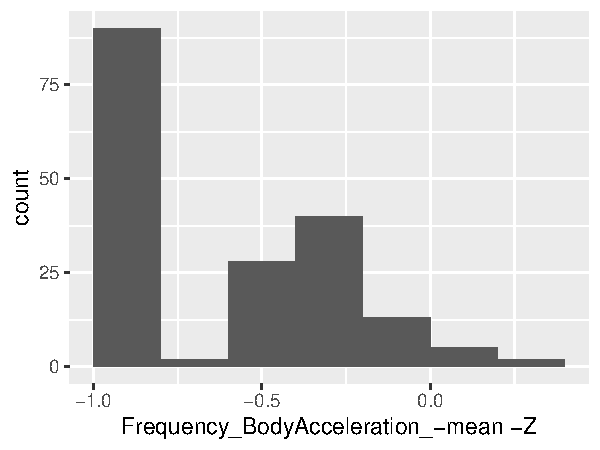
\includegraphics{codebook_tidydatasub_files/figure-latex/Var-45-Frequency-BodyAcceleration--mean--Z-1.pdf}

\end{minipage}

\noindent\makebox[\linewidth]{\rule{\textwidth}{0.4pt}}

\hypertarget{frequency_bodyacceleration_-standard-deviation--x}{%
\subsection{Frequency\_BodyAcceleration\_-Standard-Deviation
-X}\label{frequency_bodyacceleration_-standard-deviation--x}}

\begin{minipage}{0.75 \textwidth}

\begin{longtable}[]{@{}lr@{}}
\toprule
\begin{minipage}[b]{0.34\columnwidth}\raggedright
Feature\strut
\end{minipage} & \begin{minipage}[b]{0.18\columnwidth}\raggedleft
Result\strut
\end{minipage}\tabularnewline
\midrule
\endhead
\begin{minipage}[t]{0.34\columnwidth}\raggedright
Variable type\strut
\end{minipage} & \begin{minipage}[t]{0.18\columnwidth}\raggedleft
numeric\strut
\end{minipage}\tabularnewline
\begin{minipage}[t]{0.34\columnwidth}\raggedright
Number of missing obs.\strut
\end{minipage} & \begin{minipage}[t]{0.18\columnwidth}\raggedleft
0 (0 \%)\strut
\end{minipage}\tabularnewline
\begin{minipage}[t]{0.34\columnwidth}\raggedright
Number of unique values\strut
\end{minipage} & \begin{minipage}[t]{0.18\columnwidth}\raggedleft
180\strut
\end{minipage}\tabularnewline
\begin{minipage}[t]{0.34\columnwidth}\raggedright
Median\strut
\end{minipage} & \begin{minipage}[t]{0.18\columnwidth}\raggedleft
-0.75\strut
\end{minipage}\tabularnewline
\begin{minipage}[t]{0.34\columnwidth}\raggedright
1st and 3rd quartiles\strut
\end{minipage} & \begin{minipage}[t]{0.18\columnwidth}\raggedleft
-0.98; -0.2\strut
\end{minipage}\tabularnewline
\begin{minipage}[t]{0.34\columnwidth}\raggedright
Min. and max.\strut
\end{minipage} & \begin{minipage}[t]{0.18\columnwidth}\raggedleft
-1; 0.66\strut
\end{minipage}\tabularnewline
\bottomrule
\end{longtable}

\end{minipage}
\begin{minipage}{0.25 \textwidth}

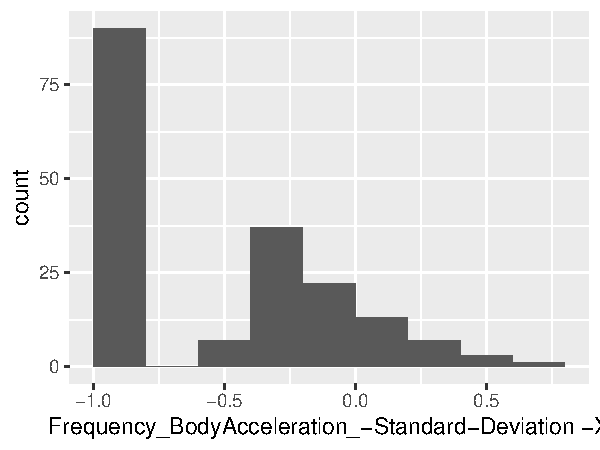
\includegraphics{codebook_tidydatasub_files/figure-latex/Var-46-Frequency-BodyAcceleration--Standard-Deviation--X-1.pdf}

\end{minipage}

\noindent\makebox[\linewidth]{\rule{\textwidth}{0.4pt}}

\hypertarget{frequency_bodyacceleration_-standard-deviation--y}{%
\subsection{Frequency\_BodyAcceleration\_-Standard-Deviation
-Y}\label{frequency_bodyacceleration_-standard-deviation--y}}

\begin{minipage}{0.75 \textwidth}

\begin{longtable}[]{@{}lr@{}}
\toprule
\begin{minipage}[b]{0.34\columnwidth}\raggedright
Feature\strut
\end{minipage} & \begin{minipage}[b]{0.20\columnwidth}\raggedleft
Result\strut
\end{minipage}\tabularnewline
\midrule
\endhead
\begin{minipage}[t]{0.34\columnwidth}\raggedright
Variable type\strut
\end{minipage} & \begin{minipage}[t]{0.20\columnwidth}\raggedleft
numeric\strut
\end{minipage}\tabularnewline
\begin{minipage}[t]{0.34\columnwidth}\raggedright
Number of missing obs.\strut
\end{minipage} & \begin{minipage}[t]{0.20\columnwidth}\raggedleft
0 (0 \%)\strut
\end{minipage}\tabularnewline
\begin{minipage}[t]{0.34\columnwidth}\raggedright
Number of unique values\strut
\end{minipage} & \begin{minipage}[t]{0.20\columnwidth}\raggedleft
180\strut
\end{minipage}\tabularnewline
\begin{minipage}[t]{0.34\columnwidth}\raggedright
Median\strut
\end{minipage} & \begin{minipage}[t]{0.20\columnwidth}\raggedleft
-0.51\strut
\end{minipage}\tabularnewline
\begin{minipage}[t]{0.34\columnwidth}\raggedright
1st and 3rd quartiles\strut
\end{minipage} & \begin{minipage}[t]{0.20\columnwidth}\raggedleft
-0.94; -0.08\strut
\end{minipage}\tabularnewline
\begin{minipage}[t]{0.34\columnwidth}\raggedright
Min. and max.\strut
\end{minipage} & \begin{minipage}[t]{0.20\columnwidth}\raggedleft
-0.99; 0.56\strut
\end{minipage}\tabularnewline
\bottomrule
\end{longtable}

\end{minipage}
\begin{minipage}{0.25 \textwidth}

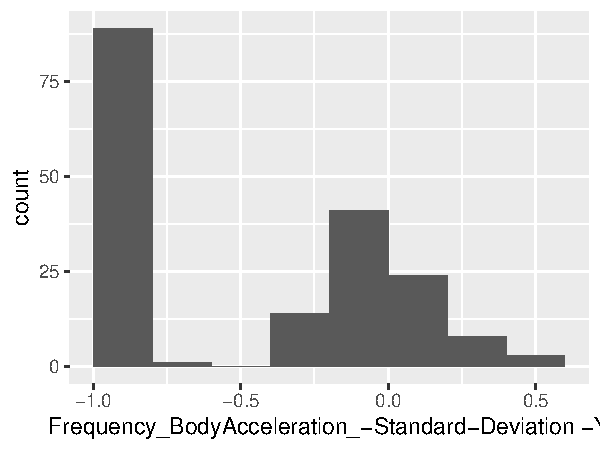
\includegraphics{codebook_tidydatasub_files/figure-latex/Var-47-Frequency-BodyAcceleration--Standard-Deviation--Y-1.pdf}

\end{minipage}

\noindent\makebox[\linewidth]{\rule{\textwidth}{0.4pt}}

\hypertarget{frequency_bodyacceleration_-standard-deviation--z}{%
\subsection{Frequency\_BodyAcceleration\_-Standard-Deviation
-Z}\label{frequency_bodyacceleration_-standard-deviation--z}}

\begin{minipage}{0.75 \textwidth}

\begin{longtable}[]{@{}lr@{}}
\toprule
\begin{minipage}[b]{0.34\columnwidth}\raggedright
Feature\strut
\end{minipage} & \begin{minipage}[b]{0.20\columnwidth}\raggedleft
Result\strut
\end{minipage}\tabularnewline
\midrule
\endhead
\begin{minipage}[t]{0.34\columnwidth}\raggedright
Variable type\strut
\end{minipage} & \begin{minipage}[t]{0.20\columnwidth}\raggedleft
numeric\strut
\end{minipage}\tabularnewline
\begin{minipage}[t]{0.34\columnwidth}\raggedright
Number of missing obs.\strut
\end{minipage} & \begin{minipage}[t]{0.20\columnwidth}\raggedleft
0 (0 \%)\strut
\end{minipage}\tabularnewline
\begin{minipage}[t]{0.34\columnwidth}\raggedright
Number of unique values\strut
\end{minipage} & \begin{minipage}[t]{0.20\columnwidth}\raggedleft
180\strut
\end{minipage}\tabularnewline
\begin{minipage}[t]{0.34\columnwidth}\raggedright
Median\strut
\end{minipage} & \begin{minipage}[t]{0.20\columnwidth}\raggedleft
-0.64\strut
\end{minipage}\tabularnewline
\begin{minipage}[t]{0.34\columnwidth}\raggedright
1st and 3rd quartiles\strut
\end{minipage} & \begin{minipage}[t]{0.20\columnwidth}\raggedleft
-0.95; -0.27\strut
\end{minipage}\tabularnewline
\begin{minipage}[t]{0.34\columnwidth}\raggedright
Min. and max.\strut
\end{minipage} & \begin{minipage}[t]{0.20\columnwidth}\raggedleft
-0.99; 0.69\strut
\end{minipage}\tabularnewline
\bottomrule
\end{longtable}

\end{minipage}
\begin{minipage}{0.25 \textwidth}

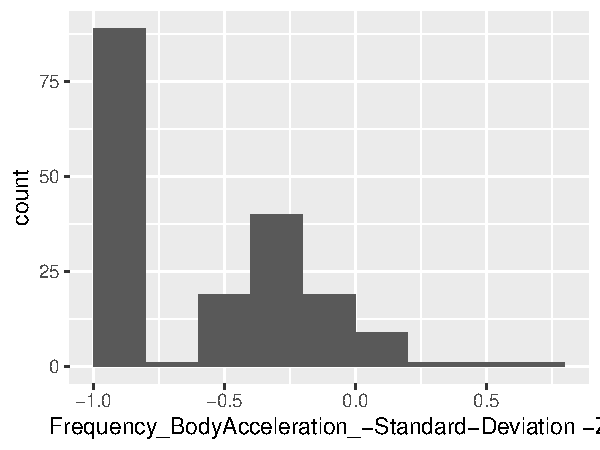
\includegraphics{codebook_tidydatasub_files/figure-latex/Var-48-Frequency-BodyAcceleration--Standard-Deviation--Z-1.pdf}

\end{minipage}

\noindent\makebox[\linewidth]{\rule{\textwidth}{0.4pt}}

\hypertarget{frequency_bodyacceleration_-meanfreq--x}{%
\subsection{Frequency\_BodyAcceleration\_-meanFreq
-X}\label{frequency_bodyacceleration_-meanfreq--x}}

\begin{minipage}{0.75 \textwidth}

\begin{longtable}[]{@{}lr@{}}
\toprule
\begin{minipage}[b]{0.34\columnwidth}\raggedright
Feature\strut
\end{minipage} & \begin{minipage}[b]{0.20\columnwidth}\raggedleft
Result\strut
\end{minipage}\tabularnewline
\midrule
\endhead
\begin{minipage}[t]{0.34\columnwidth}\raggedright
Variable type\strut
\end{minipage} & \begin{minipage}[t]{0.20\columnwidth}\raggedleft
numeric\strut
\end{minipage}\tabularnewline
\begin{minipage}[t]{0.34\columnwidth}\raggedright
Number of missing obs.\strut
\end{minipage} & \begin{minipage}[t]{0.20\columnwidth}\raggedleft
0 (0 \%)\strut
\end{minipage}\tabularnewline
\begin{minipage}[t]{0.34\columnwidth}\raggedright
Number of unique values\strut
\end{minipage} & \begin{minipage}[t]{0.20\columnwidth}\raggedleft
180\strut
\end{minipage}\tabularnewline
\begin{minipage}[t]{0.34\columnwidth}\raggedright
Median\strut
\end{minipage} & \begin{minipage}[t]{0.20\columnwidth}\raggedleft
-0.26\strut
\end{minipage}\tabularnewline
\begin{minipage}[t]{0.34\columnwidth}\raggedright
1st and 3rd quartiles\strut
\end{minipage} & \begin{minipage}[t]{0.20\columnwidth}\raggedleft
-0.39; -0.06\strut
\end{minipage}\tabularnewline
\begin{minipage}[t]{0.34\columnwidth}\raggedright
Min. and max.\strut
\end{minipage} & \begin{minipage}[t]{0.20\columnwidth}\raggedleft
-0.64; 0.16\strut
\end{minipage}\tabularnewline
\bottomrule
\end{longtable}

\end{minipage}
\begin{minipage}{0.25 \textwidth}

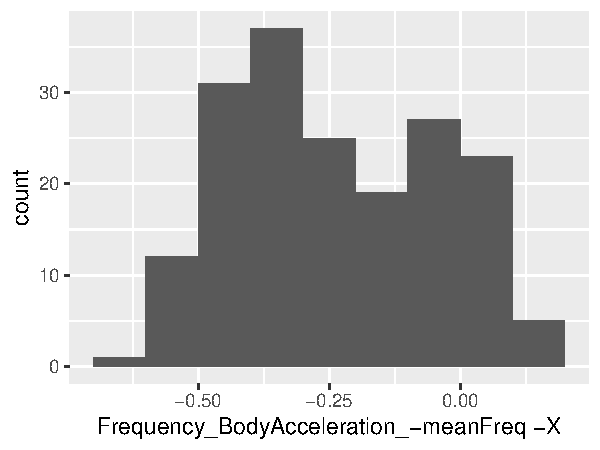
\includegraphics{codebook_tidydatasub_files/figure-latex/Var-49-Frequency-BodyAcceleration--meanFreq--X-1.pdf}

\end{minipage}

\noindent\makebox[\linewidth]{\rule{\textwidth}{0.4pt}}

\hypertarget{frequency_bodyacceleration_-meanfreq--y}{%
\subsection{Frequency\_BodyAcceleration\_-meanFreq
-Y}\label{frequency_bodyacceleration_-meanfreq--y}}

\begin{minipage}{0.75 \textwidth}

\begin{longtable}[]{@{}lr@{}}
\toprule
\begin{minipage}[b]{0.34\columnwidth}\raggedright
Feature\strut
\end{minipage} & \begin{minipage}[b]{0.18\columnwidth}\raggedleft
Result\strut
\end{minipage}\tabularnewline
\midrule
\endhead
\begin{minipage}[t]{0.34\columnwidth}\raggedright
Variable type\strut
\end{minipage} & \begin{minipage}[t]{0.18\columnwidth}\raggedleft
numeric\strut
\end{minipage}\tabularnewline
\begin{minipage}[t]{0.34\columnwidth}\raggedright
Number of missing obs.\strut
\end{minipage} & \begin{minipage}[t]{0.18\columnwidth}\raggedleft
0 (0 \%)\strut
\end{minipage}\tabularnewline
\begin{minipage}[t]{0.34\columnwidth}\raggedright
Number of unique values\strut
\end{minipage} & \begin{minipage}[t]{0.18\columnwidth}\raggedleft
180\strut
\end{minipage}\tabularnewline
\begin{minipage}[t]{0.34\columnwidth}\raggedright
Median\strut
\end{minipage} & \begin{minipage}[t]{0.18\columnwidth}\raggedleft
0.01\strut
\end{minipage}\tabularnewline
\begin{minipage}[t]{0.34\columnwidth}\raggedright
1st and 3rd quartiles\strut
\end{minipage} & \begin{minipage}[t]{0.18\columnwidth}\raggedleft
-0.08; 0.09\strut
\end{minipage}\tabularnewline
\begin{minipage}[t]{0.34\columnwidth}\raggedright
Min. and max.\strut
\end{minipage} & \begin{minipage}[t]{0.18\columnwidth}\raggedleft
-0.38; 0.47\strut
\end{minipage}\tabularnewline
\bottomrule
\end{longtable}

\end{minipage}
\begin{minipage}{0.25 \textwidth}

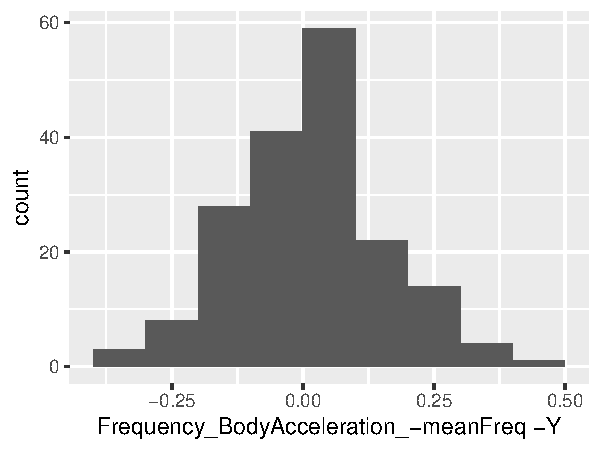
\includegraphics{codebook_tidydatasub_files/figure-latex/Var-50-Frequency-BodyAcceleration--meanFreq--Y-1.pdf}

\end{minipage}

\noindent\makebox[\linewidth]{\rule{\textwidth}{0.4pt}}

\hypertarget{frequency_bodyacceleration_-meanfreq--z}{%
\subsection{Frequency\_BodyAcceleration\_-meanFreq
-Z}\label{frequency_bodyacceleration_-meanfreq--z}}

\begin{minipage}{0.75 \textwidth}

\begin{longtable}[]{@{}lr@{}}
\toprule
\begin{minipage}[b]{0.34\columnwidth}\raggedright
Feature\strut
\end{minipage} & \begin{minipage}[b]{0.18\columnwidth}\raggedleft
Result\strut
\end{minipage}\tabularnewline
\midrule
\endhead
\begin{minipage}[t]{0.34\columnwidth}\raggedright
Variable type\strut
\end{minipage} & \begin{minipage}[t]{0.18\columnwidth}\raggedleft
numeric\strut
\end{minipage}\tabularnewline
\begin{minipage}[t]{0.34\columnwidth}\raggedright
Number of missing obs.\strut
\end{minipage} & \begin{minipage}[t]{0.18\columnwidth}\raggedleft
0 (0 \%)\strut
\end{minipage}\tabularnewline
\begin{minipage}[t]{0.34\columnwidth}\raggedright
Number of unique values\strut
\end{minipage} & \begin{minipage}[t]{0.18\columnwidth}\raggedleft
180\strut
\end{minipage}\tabularnewline
\begin{minipage}[t]{0.34\columnwidth}\raggedright
Median\strut
\end{minipage} & \begin{minipage}[t]{0.18\columnwidth}\raggedleft
0.07\strut
\end{minipage}\tabularnewline
\begin{minipage}[t]{0.34\columnwidth}\raggedright
1st and 3rd quartiles\strut
\end{minipage} & \begin{minipage}[t]{0.18\columnwidth}\raggedleft
-0.04; 0.18\strut
\end{minipage}\tabularnewline
\begin{minipage}[t]{0.34\columnwidth}\raggedright
Min. and max.\strut
\end{minipage} & \begin{minipage}[t]{0.18\columnwidth}\raggedleft
-0.52; 0.4\strut
\end{minipage}\tabularnewline
\bottomrule
\end{longtable}

\end{minipage}
\begin{minipage}{0.25 \textwidth}

\includegraphics{codebook_tidydatasub_files/figure-latex/Var-51-Frequency-BodyAcceleration--meanFreq--Z-1.pdf}

\end{minipage}

\noindent\makebox[\linewidth]{\rule{\textwidth}{0.4pt}}

\hypertarget{frequency_bodyacceleration_jerk-mean--x}{%
\subsection{Frequency\_BodyAcceleration\_Jerk-mean
-X}\label{frequency_bodyacceleration_jerk-mean--x}}

\begin{minipage}{0.75 \textwidth}

\begin{longtable}[]{@{}lr@{}}
\toprule
\begin{minipage}[b]{0.34\columnwidth}\raggedright
Feature\strut
\end{minipage} & \begin{minipage}[b]{0.20\columnwidth}\raggedleft
Result\strut
\end{minipage}\tabularnewline
\midrule
\endhead
\begin{minipage}[t]{0.34\columnwidth}\raggedright
Variable type\strut
\end{minipage} & \begin{minipage}[t]{0.20\columnwidth}\raggedleft
numeric\strut
\end{minipage}\tabularnewline
\begin{minipage}[t]{0.34\columnwidth}\raggedright
Number of missing obs.\strut
\end{minipage} & \begin{minipage}[t]{0.20\columnwidth}\raggedleft
0 (0 \%)\strut
\end{minipage}\tabularnewline
\begin{minipage}[t]{0.34\columnwidth}\raggedright
Number of unique values\strut
\end{minipage} & \begin{minipage}[t]{0.20\columnwidth}\raggedleft
180\strut
\end{minipage}\tabularnewline
\begin{minipage}[t]{0.34\columnwidth}\raggedright
Median\strut
\end{minipage} & \begin{minipage}[t]{0.20\columnwidth}\raggedleft
-0.81\strut
\end{minipage}\tabularnewline
\begin{minipage}[t]{0.34\columnwidth}\raggedright
1st and 3rd quartiles\strut
\end{minipage} & \begin{minipage}[t]{0.20\columnwidth}\raggedleft
-0.98; -0.28\strut
\end{minipage}\tabularnewline
\begin{minipage}[t]{0.34\columnwidth}\raggedright
Min. and max.\strut
\end{minipage} & \begin{minipage}[t]{0.20\columnwidth}\raggedleft
-0.99; 0.47\strut
\end{minipage}\tabularnewline
\bottomrule
\end{longtable}

\end{minipage}
\begin{minipage}{0.25 \textwidth}

\includegraphics{codebook_tidydatasub_files/figure-latex/Var-52-Frequency-BodyAcceleration-Jerk-mean--X-1.pdf}

\end{minipage}

\noindent\makebox[\linewidth]{\rule{\textwidth}{0.4pt}}

\hypertarget{frequency_bodyacceleration_jerk-mean--y}{%
\subsection{Frequency\_BodyAcceleration\_Jerk-mean
-Y}\label{frequency_bodyacceleration_jerk-mean--y}}

\begin{minipage}{0.75 \textwidth}

\begin{longtable}[]{@{}lr@{}}
\toprule
\begin{minipage}[b]{0.34\columnwidth}\raggedright
Feature\strut
\end{minipage} & \begin{minipage}[b]{0.18\columnwidth}\raggedleft
Result\strut
\end{minipage}\tabularnewline
\midrule
\endhead
\begin{minipage}[t]{0.34\columnwidth}\raggedright
Variable type\strut
\end{minipage} & \begin{minipage}[t]{0.18\columnwidth}\raggedleft
numeric\strut
\end{minipage}\tabularnewline
\begin{minipage}[t]{0.34\columnwidth}\raggedright
Number of missing obs.\strut
\end{minipage} & \begin{minipage}[t]{0.18\columnwidth}\raggedleft
0 (0 \%)\strut
\end{minipage}\tabularnewline
\begin{minipage}[t]{0.34\columnwidth}\raggedright
Number of unique values\strut
\end{minipage} & \begin{minipage}[t]{0.18\columnwidth}\raggedleft
180\strut
\end{minipage}\tabularnewline
\begin{minipage}[t]{0.34\columnwidth}\raggedright
Median\strut
\end{minipage} & \begin{minipage}[t]{0.18\columnwidth}\raggedleft
-0.78\strut
\end{minipage}\tabularnewline
\begin{minipage}[t]{0.34\columnwidth}\raggedright
1st and 3rd quartiles\strut
\end{minipage} & \begin{minipage}[t]{0.18\columnwidth}\raggedleft
-0.97; -0.2\strut
\end{minipage}\tabularnewline
\begin{minipage}[t]{0.34\columnwidth}\raggedright
Min. and max.\strut
\end{minipage} & \begin{minipage}[t]{0.18\columnwidth}\raggedleft
-0.99; 0.28\strut
\end{minipage}\tabularnewline
\bottomrule
\end{longtable}

\end{minipage}
\begin{minipage}{0.25 \textwidth}

\includegraphics{codebook_tidydatasub_files/figure-latex/Var-53-Frequency-BodyAcceleration-Jerk-mean--Y-1.pdf}

\end{minipage}

\noindent\makebox[\linewidth]{\rule{\textwidth}{0.4pt}}

\hypertarget{frequency_bodyacceleration_jerk-mean--z}{%
\subsection{Frequency\_BodyAcceleration\_Jerk-mean
-Z}\label{frequency_bodyacceleration_jerk-mean--z}}

\begin{minipage}{0.75 \textwidth}

\begin{longtable}[]{@{}lr@{}}
\toprule
\begin{minipage}[b]{0.34\columnwidth}\raggedright
Feature\strut
\end{minipage} & \begin{minipage}[b]{0.20\columnwidth}\raggedleft
Result\strut
\end{minipage}\tabularnewline
\midrule
\endhead
\begin{minipage}[t]{0.34\columnwidth}\raggedright
Variable type\strut
\end{minipage} & \begin{minipage}[t]{0.20\columnwidth}\raggedleft
numeric\strut
\end{minipage}\tabularnewline
\begin{minipage}[t]{0.34\columnwidth}\raggedright
Number of missing obs.\strut
\end{minipage} & \begin{minipage}[t]{0.20\columnwidth}\raggedleft
0 (0 \%)\strut
\end{minipage}\tabularnewline
\begin{minipage}[t]{0.34\columnwidth}\raggedright
Number of unique values\strut
\end{minipage} & \begin{minipage}[t]{0.20\columnwidth}\raggedleft
180\strut
\end{minipage}\tabularnewline
\begin{minipage}[t]{0.34\columnwidth}\raggedright
Median\strut
\end{minipage} & \begin{minipage}[t]{0.20\columnwidth}\raggedleft
-0.87\strut
\end{minipage}\tabularnewline
\begin{minipage}[t]{0.34\columnwidth}\raggedright
1st and 3rd quartiles\strut
\end{minipage} & \begin{minipage}[t]{0.20\columnwidth}\raggedleft
-0.98; -0.47\strut
\end{minipage}\tabularnewline
\begin{minipage}[t]{0.34\columnwidth}\raggedright
Min. and max.\strut
\end{minipage} & \begin{minipage}[t]{0.20\columnwidth}\raggedleft
-0.99; 0.16\strut
\end{minipage}\tabularnewline
\bottomrule
\end{longtable}

\end{minipage}
\begin{minipage}{0.25 \textwidth}

\includegraphics{codebook_tidydatasub_files/figure-latex/Var-54-Frequency-BodyAcceleration-Jerk-mean--Z-1.pdf}

\end{minipage}

\noindent\makebox[\linewidth]{\rule{\textwidth}{0.4pt}}

\hypertarget{frequency_bodyacceleration_jerk-standard-deviation--x}{%
\subsection{Frequency\_BodyAcceleration\_Jerk-Standard-Deviation
-X}\label{frequency_bodyacceleration_jerk-standard-deviation--x}}

\begin{minipage}{0.75 \textwidth}

\begin{longtable}[]{@{}lr@{}}
\toprule
\begin{minipage}[b]{0.34\columnwidth}\raggedright
Feature\strut
\end{minipage} & \begin{minipage}[b]{0.20\columnwidth}\raggedleft
Result\strut
\end{minipage}\tabularnewline
\midrule
\endhead
\begin{minipage}[t]{0.34\columnwidth}\raggedright
Variable type\strut
\end{minipage} & \begin{minipage}[t]{0.20\columnwidth}\raggedleft
numeric\strut
\end{minipage}\tabularnewline
\begin{minipage}[t]{0.34\columnwidth}\raggedright
Number of missing obs.\strut
\end{minipage} & \begin{minipage}[t]{0.20\columnwidth}\raggedleft
0 (0 \%)\strut
\end{minipage}\tabularnewline
\begin{minipage}[t]{0.34\columnwidth}\raggedright
Number of unique values\strut
\end{minipage} & \begin{minipage}[t]{0.20\columnwidth}\raggedleft
180\strut
\end{minipage}\tabularnewline
\begin{minipage}[t]{0.34\columnwidth}\raggedright
Median\strut
\end{minipage} & \begin{minipage}[t]{0.20\columnwidth}\raggedleft
-0.83\strut
\end{minipage}\tabularnewline
\begin{minipage}[t]{0.34\columnwidth}\raggedright
1st and 3rd quartiles\strut
\end{minipage} & \begin{minipage}[t]{0.20\columnwidth}\raggedleft
-0.98; -0.25\strut
\end{minipage}\tabularnewline
\begin{minipage}[t]{0.34\columnwidth}\raggedright
Min. and max.\strut
\end{minipage} & \begin{minipage}[t]{0.20\columnwidth}\raggedleft
-1; 0.48\strut
\end{minipage}\tabularnewline
\bottomrule
\end{longtable}

\end{minipage}
\begin{minipage}{0.25 \textwidth}

\includegraphics{codebook_tidydatasub_files/figure-latex/Var-55-Frequency-BodyAcceleration-Jerk-Standard-Deviation--X-1.pdf}

\end{minipage}

\noindent\makebox[\linewidth]{\rule{\textwidth}{0.4pt}}

\hypertarget{frequency_bodyacceleration_jerk-standard-deviation--y}{%
\subsection{Frequency\_BodyAcceleration\_Jerk-Standard-Deviation
-Y}\label{frequency_bodyacceleration_jerk-standard-deviation--y}}

\begin{minipage}{0.75 \textwidth}

\begin{longtable}[]{@{}lr@{}}
\toprule
\begin{minipage}[b]{0.34\columnwidth}\raggedright
Feature\strut
\end{minipage} & \begin{minipage}[b]{0.20\columnwidth}\raggedleft
Result\strut
\end{minipage}\tabularnewline
\midrule
\endhead
\begin{minipage}[t]{0.34\columnwidth}\raggedright
Variable type\strut
\end{minipage} & \begin{minipage}[t]{0.20\columnwidth}\raggedleft
numeric\strut
\end{minipage}\tabularnewline
\begin{minipage}[t]{0.34\columnwidth}\raggedright
Number of missing obs.\strut
\end{minipage} & \begin{minipage}[t]{0.20\columnwidth}\raggedleft
0 (0 \%)\strut
\end{minipage}\tabularnewline
\begin{minipage}[t]{0.34\columnwidth}\raggedright
Number of unique values\strut
\end{minipage} & \begin{minipage}[t]{0.20\columnwidth}\raggedleft
180\strut
\end{minipage}\tabularnewline
\begin{minipage}[t]{0.34\columnwidth}\raggedright
Median\strut
\end{minipage} & \begin{minipage}[t]{0.20\columnwidth}\raggedleft
-0.79\strut
\end{minipage}\tabularnewline
\begin{minipage}[t]{0.34\columnwidth}\raggedright
1st and 3rd quartiles\strut
\end{minipage} & \begin{minipage}[t]{0.20\columnwidth}\raggedleft
-0.97; -0.17\strut
\end{minipage}\tabularnewline
\begin{minipage}[t]{0.34\columnwidth}\raggedright
Min. and max.\strut
\end{minipage} & \begin{minipage}[t]{0.20\columnwidth}\raggedleft
-0.99; 0.35\strut
\end{minipage}\tabularnewline
\bottomrule
\end{longtable}

\end{minipage}
\begin{minipage}{0.25 \textwidth}

\includegraphics{codebook_tidydatasub_files/figure-latex/Var-56-Frequency-BodyAcceleration-Jerk-Standard-Deviation--Y-1.pdf}

\end{minipage}

\noindent\makebox[\linewidth]{\rule{\textwidth}{0.4pt}}

\hypertarget{frequency_bodyacceleration_jerk-standard-deviation--z}{%
\subsection{Frequency\_BodyAcceleration\_Jerk-Standard-Deviation
-Z}\label{frequency_bodyacceleration_jerk-standard-deviation--z}}

\begin{minipage}{0.75 \textwidth}

\begin{longtable}[]{@{}lr@{}}
\toprule
\begin{minipage}[b]{0.34\columnwidth}\raggedright
Feature\strut
\end{minipage} & \begin{minipage}[b]{0.20\columnwidth}\raggedleft
Result\strut
\end{minipage}\tabularnewline
\midrule
\endhead
\begin{minipage}[t]{0.34\columnwidth}\raggedright
Variable type\strut
\end{minipage} & \begin{minipage}[t]{0.20\columnwidth}\raggedleft
numeric\strut
\end{minipage}\tabularnewline
\begin{minipage}[t]{0.34\columnwidth}\raggedright
Number of missing obs.\strut
\end{minipage} & \begin{minipage}[t]{0.20\columnwidth}\raggedleft
0 (0 \%)\strut
\end{minipage}\tabularnewline
\begin{minipage}[t]{0.34\columnwidth}\raggedright
Number of unique values\strut
\end{minipage} & \begin{minipage}[t]{0.20\columnwidth}\raggedleft
180\strut
\end{minipage}\tabularnewline
\begin{minipage}[t]{0.34\columnwidth}\raggedright
Median\strut
\end{minipage} & \begin{minipage}[t]{0.20\columnwidth}\raggedleft
-0.9\strut
\end{minipage}\tabularnewline
\begin{minipage}[t]{0.34\columnwidth}\raggedright
1st and 3rd quartiles\strut
\end{minipage} & \begin{minipage}[t]{0.20\columnwidth}\raggedleft
-0.98; -0.54\strut
\end{minipage}\tabularnewline
\begin{minipage}[t]{0.34\columnwidth}\raggedright
Min. and max.\strut
\end{minipage} & \begin{minipage}[t]{0.20\columnwidth}\raggedleft
-0.99; -0.01\strut
\end{minipage}\tabularnewline
\bottomrule
\end{longtable}

\end{minipage}
\begin{minipage}{0.25 \textwidth}

\includegraphics{codebook_tidydatasub_files/figure-latex/Var-57-Frequency-BodyAcceleration-Jerk-Standard-Deviation--Z-1.pdf}

\end{minipage}

\noindent\makebox[\linewidth]{\rule{\textwidth}{0.4pt}}

\hypertarget{frequency_bodyacceleration_jerk-meanfreq--x}{%
\subsection{Frequency\_BodyAcceleration\_Jerk-meanFreq
-X}\label{frequency_bodyacceleration_jerk-meanfreq--x}}

\begin{minipage}{0.75 \textwidth}

\begin{longtable}[]{@{}lr@{}}
\toprule
\begin{minipage}[b]{0.34\columnwidth}\raggedright
Feature\strut
\end{minipage} & \begin{minipage}[b]{0.18\columnwidth}\raggedleft
Result\strut
\end{minipage}\tabularnewline
\midrule
\endhead
\begin{minipage}[t]{0.34\columnwidth}\raggedright
Variable type\strut
\end{minipage} & \begin{minipage}[t]{0.18\columnwidth}\raggedleft
numeric\strut
\end{minipage}\tabularnewline
\begin{minipage}[t]{0.34\columnwidth}\raggedright
Number of missing obs.\strut
\end{minipage} & \begin{minipage}[t]{0.18\columnwidth}\raggedleft
0 (0 \%)\strut
\end{minipage}\tabularnewline
\begin{minipage}[t]{0.34\columnwidth}\raggedright
Number of unique values\strut
\end{minipage} & \begin{minipage}[t]{0.18\columnwidth}\raggedleft
180\strut
\end{minipage}\tabularnewline
\begin{minipage}[t]{0.34\columnwidth}\raggedright
Median\strut
\end{minipage} & \begin{minipage}[t]{0.18\columnwidth}\raggedleft
-0.06\strut
\end{minipage}\tabularnewline
\begin{minipage}[t]{0.34\columnwidth}\raggedright
1st and 3rd quartiles\strut
\end{minipage} & \begin{minipage}[t]{0.18\columnwidth}\raggedleft
-0.29; 0.18\strut
\end{minipage}\tabularnewline
\begin{minipage}[t]{0.34\columnwidth}\raggedright
Min. and max.\strut
\end{minipage} & \begin{minipage}[t]{0.18\columnwidth}\raggedleft
-0.58; 0.33\strut
\end{minipage}\tabularnewline
\bottomrule
\end{longtable}

\end{minipage}
\begin{minipage}{0.25 \textwidth}

\includegraphics{codebook_tidydatasub_files/figure-latex/Var-58-Frequency-BodyAcceleration-Jerk-meanFreq--X-1.pdf}

\end{minipage}

\noindent\makebox[\linewidth]{\rule{\textwidth}{0.4pt}}

\hypertarget{frequency_bodyacceleration_jerk-meanfreq--y}{%
\subsection{Frequency\_BodyAcceleration\_Jerk-meanFreq
-Y}\label{frequency_bodyacceleration_jerk-meanfreq--y}}

\begin{minipage}{0.75 \textwidth}

\begin{longtable}[]{@{}lr@{}}
\toprule
\begin{minipage}[b]{0.34\columnwidth}\raggedright
Feature\strut
\end{minipage} & \begin{minipage}[b]{0.18\columnwidth}\raggedleft
Result\strut
\end{minipage}\tabularnewline
\midrule
\endhead
\begin{minipage}[t]{0.34\columnwidth}\raggedright
Variable type\strut
\end{minipage} & \begin{minipage}[t]{0.18\columnwidth}\raggedleft
numeric\strut
\end{minipage}\tabularnewline
\begin{minipage}[t]{0.34\columnwidth}\raggedright
Number of missing obs.\strut
\end{minipage} & \begin{minipage}[t]{0.18\columnwidth}\raggedleft
0 (0 \%)\strut
\end{minipage}\tabularnewline
\begin{minipage}[t]{0.34\columnwidth}\raggedright
Number of unique values\strut
\end{minipage} & \begin{minipage}[t]{0.18\columnwidth}\raggedleft
180\strut
\end{minipage}\tabularnewline
\begin{minipage}[t]{0.34\columnwidth}\raggedright
Median\strut
\end{minipage} & \begin{minipage}[t]{0.18\columnwidth}\raggedleft
-0.23\strut
\end{minipage}\tabularnewline
\begin{minipage}[t]{0.34\columnwidth}\raggedright
1st and 3rd quartiles\strut
\end{minipage} & \begin{minipage}[t]{0.18\columnwidth}\raggedleft
-0.4; -0.05\strut
\end{minipage}\tabularnewline
\begin{minipage}[t]{0.34\columnwidth}\raggedright
Min. and max.\strut
\end{minipage} & \begin{minipage}[t]{0.18\columnwidth}\raggedleft
-0.6; 0.2\strut
\end{minipage}\tabularnewline
\bottomrule
\end{longtable}

\end{minipage}
\begin{minipage}{0.25 \textwidth}

\includegraphics{codebook_tidydatasub_files/figure-latex/Var-59-Frequency-BodyAcceleration-Jerk-meanFreq--Y-1.pdf}

\end{minipage}

\noindent\makebox[\linewidth]{\rule{\textwidth}{0.4pt}}

\hypertarget{frequency_bodyacceleration_jerk-meanfreq--z}{%
\subsection{Frequency\_BodyAcceleration\_Jerk-meanFreq
-Z}\label{frequency_bodyacceleration_jerk-meanfreq--z}}

\begin{minipage}{0.75 \textwidth}

\begin{longtable}[]{@{}lr@{}}
\toprule
\begin{minipage}[b]{0.34\columnwidth}\raggedright
Feature\strut
\end{minipage} & \begin{minipage}[b]{0.18\columnwidth}\raggedleft
Result\strut
\end{minipage}\tabularnewline
\midrule
\endhead
\begin{minipage}[t]{0.34\columnwidth}\raggedright
Variable type\strut
\end{minipage} & \begin{minipage}[t]{0.18\columnwidth}\raggedleft
numeric\strut
\end{minipage}\tabularnewline
\begin{minipage}[t]{0.34\columnwidth}\raggedright
Number of missing obs.\strut
\end{minipage} & \begin{minipage}[t]{0.18\columnwidth}\raggedleft
0 (0 \%)\strut
\end{minipage}\tabularnewline
\begin{minipage}[t]{0.34\columnwidth}\raggedright
Number of unique values\strut
\end{minipage} & \begin{minipage}[t]{0.18\columnwidth}\raggedleft
180\strut
\end{minipage}\tabularnewline
\begin{minipage}[t]{0.34\columnwidth}\raggedright
Median\strut
\end{minipage} & \begin{minipage}[t]{0.18\columnwidth}\raggedleft
-0.09\strut
\end{minipage}\tabularnewline
\begin{minipage}[t]{0.34\columnwidth}\raggedright
1st and 3rd quartiles\strut
\end{minipage} & \begin{minipage}[t]{0.18\columnwidth}\raggedleft
-0.31; 0.04\strut
\end{minipage}\tabularnewline
\begin{minipage}[t]{0.34\columnwidth}\raggedright
Min. and max.\strut
\end{minipage} & \begin{minipage}[t]{0.18\columnwidth}\raggedleft
-0.63; 0.23\strut
\end{minipage}\tabularnewline
\bottomrule
\end{longtable}

\end{minipage}
\begin{minipage}{0.25 \textwidth}

\includegraphics{codebook_tidydatasub_files/figure-latex/Var-60-Frequency-BodyAcceleration-Jerk-meanFreq--Z-1.pdf}

\end{minipage}

\noindent\makebox[\linewidth]{\rule{\textwidth}{0.4pt}}

\hypertarget{frequency_bodygyroscope-mean--x}{%
\subsection{Frequency\_BodyGyroscope-mean
-X}\label{frequency_bodygyroscope-mean--x}}

\begin{minipage}{0.75 \textwidth}

\begin{longtable}[]{@{}lr@{}}
\toprule
\begin{minipage}[b]{0.34\columnwidth}\raggedright
Feature\strut
\end{minipage} & \begin{minipage}[b]{0.20\columnwidth}\raggedleft
Result\strut
\end{minipage}\tabularnewline
\midrule
\endhead
\begin{minipage}[t]{0.34\columnwidth}\raggedright
Variable type\strut
\end{minipage} & \begin{minipage}[t]{0.20\columnwidth}\raggedleft
numeric\strut
\end{minipage}\tabularnewline
\begin{minipage}[t]{0.34\columnwidth}\raggedright
Number of missing obs.\strut
\end{minipage} & \begin{minipage}[t]{0.20\columnwidth}\raggedleft
0 (0 \%)\strut
\end{minipage}\tabularnewline
\begin{minipage}[t]{0.34\columnwidth}\raggedright
Number of unique values\strut
\end{minipage} & \begin{minipage}[t]{0.20\columnwidth}\raggedleft
180\strut
\end{minipage}\tabularnewline
\begin{minipage}[t]{0.34\columnwidth}\raggedright
Median\strut
\end{minipage} & \begin{minipage}[t]{0.20\columnwidth}\raggedleft
-0.73\strut
\end{minipage}\tabularnewline
\begin{minipage}[t]{0.34\columnwidth}\raggedright
1st and 3rd quartiles\strut
\end{minipage} & \begin{minipage}[t]{0.20\columnwidth}\raggedleft
-0.97; -0.34\strut
\end{minipage}\tabularnewline
\begin{minipage}[t]{0.34\columnwidth}\raggedright
Min. and max.\strut
\end{minipage} & \begin{minipage}[t]{0.20\columnwidth}\raggedleft
-0.99; 0.47\strut
\end{minipage}\tabularnewline
\bottomrule
\end{longtable}

\end{minipage}
\begin{minipage}{0.25 \textwidth}

\includegraphics{codebook_tidydatasub_files/figure-latex/Var-61-Frequency-BodyGyroscope-mean--X-1.pdf}

\end{minipage}

\noindent\makebox[\linewidth]{\rule{\textwidth}{0.4pt}}

\hypertarget{frequency_bodygyroscope-mean--y}{%
\subsection{Frequency\_BodyGyroscope-mean
-Y}\label{frequency_bodygyroscope-mean--y}}

\begin{minipage}{0.75 \textwidth}

\begin{longtable}[]{@{}lr@{}}
\toprule
\begin{minipage}[b]{0.34\columnwidth}\raggedright
Feature\strut
\end{minipage} & \begin{minipage}[b]{0.20\columnwidth}\raggedleft
Result\strut
\end{minipage}\tabularnewline
\midrule
\endhead
\begin{minipage}[t]{0.34\columnwidth}\raggedright
Variable type\strut
\end{minipage} & \begin{minipage}[t]{0.20\columnwidth}\raggedleft
numeric\strut
\end{minipage}\tabularnewline
\begin{minipage}[t]{0.34\columnwidth}\raggedright
Number of missing obs.\strut
\end{minipage} & \begin{minipage}[t]{0.20\columnwidth}\raggedleft
0 (0 \%)\strut
\end{minipage}\tabularnewline
\begin{minipage}[t]{0.34\columnwidth}\raggedright
Number of unique values\strut
\end{minipage} & \begin{minipage}[t]{0.20\columnwidth}\raggedleft
180\strut
\end{minipage}\tabularnewline
\begin{minipage}[t]{0.34\columnwidth}\raggedright
Median\strut
\end{minipage} & \begin{minipage}[t]{0.20\columnwidth}\raggedleft
-0.81\strut
\end{minipage}\tabularnewline
\begin{minipage}[t]{0.34\columnwidth}\raggedright
1st and 3rd quartiles\strut
\end{minipage} & \begin{minipage}[t]{0.20\columnwidth}\raggedleft
-0.97; -0.45\strut
\end{minipage}\tabularnewline
\begin{minipage}[t]{0.34\columnwidth}\raggedright
Min. and max.\strut
\end{minipage} & \begin{minipage}[t]{0.20\columnwidth}\raggedleft
-0.99; 0.33\strut
\end{minipage}\tabularnewline
\bottomrule
\end{longtable}

\end{minipage}
\begin{minipage}{0.25 \textwidth}

\includegraphics{codebook_tidydatasub_files/figure-latex/Var-62-Frequency-BodyGyroscope-mean--Y-1.pdf}

\end{minipage}

\noindent\makebox[\linewidth]{\rule{\textwidth}{0.4pt}}

\hypertarget{frequency_bodygyroscope-mean--z}{%
\subsection{Frequency\_BodyGyroscope-mean
-Z}\label{frequency_bodygyroscope-mean--z}}

\begin{minipage}{0.75 \textwidth}

\begin{longtable}[]{@{}lr@{}}
\toprule
\begin{minipage}[b]{0.34\columnwidth}\raggedright
Feature\strut
\end{minipage} & \begin{minipage}[b]{0.20\columnwidth}\raggedleft
Result\strut
\end{minipage}\tabularnewline
\midrule
\endhead
\begin{minipage}[t]{0.34\columnwidth}\raggedright
Variable type\strut
\end{minipage} & \begin{minipage}[t]{0.20\columnwidth}\raggedleft
numeric\strut
\end{minipage}\tabularnewline
\begin{minipage}[t]{0.34\columnwidth}\raggedright
Number of missing obs.\strut
\end{minipage} & \begin{minipage}[t]{0.20\columnwidth}\raggedleft
0 (0 \%)\strut
\end{minipage}\tabularnewline
\begin{minipage}[t]{0.34\columnwidth}\raggedright
Number of unique values\strut
\end{minipage} & \begin{minipage}[t]{0.20\columnwidth}\raggedleft
180\strut
\end{minipage}\tabularnewline
\begin{minipage}[t]{0.34\columnwidth}\raggedright
Median\strut
\end{minipage} & \begin{minipage}[t]{0.20\columnwidth}\raggedleft
-0.79\strut
\end{minipage}\tabularnewline
\begin{minipage}[t]{0.34\columnwidth}\raggedright
1st and 3rd quartiles\strut
\end{minipage} & \begin{minipage}[t]{0.20\columnwidth}\raggedleft
-0.96; -0.26\strut
\end{minipage}\tabularnewline
\begin{minipage}[t]{0.34\columnwidth}\raggedright
Min. and max.\strut
\end{minipage} & \begin{minipage}[t]{0.20\columnwidth}\raggedleft
-0.99; 0.49\strut
\end{minipage}\tabularnewline
\bottomrule
\end{longtable}

\end{minipage}
\begin{minipage}{0.25 \textwidth}

\includegraphics{codebook_tidydatasub_files/figure-latex/Var-63-Frequency-BodyGyroscope-mean--Z-1.pdf}

\end{minipage}

\noindent\makebox[\linewidth]{\rule{\textwidth}{0.4pt}}

\hypertarget{frequency_bodygyroscope-standard-deviation--x}{%
\subsection{Frequency\_BodyGyroscope-Standard-Deviation
-X}\label{frequency_bodygyroscope-standard-deviation--x}}

\begin{minipage}{0.75 \textwidth}

\begin{longtable}[]{@{}lr@{}}
\toprule
\begin{minipage}[b]{0.34\columnwidth}\raggedright
Feature\strut
\end{minipage} & \begin{minipage}[b]{0.20\columnwidth}\raggedleft
Result\strut
\end{minipage}\tabularnewline
\midrule
\endhead
\begin{minipage}[t]{0.34\columnwidth}\raggedright
Variable type\strut
\end{minipage} & \begin{minipage}[t]{0.20\columnwidth}\raggedleft
numeric\strut
\end{minipage}\tabularnewline
\begin{minipage}[t]{0.34\columnwidth}\raggedright
Number of missing obs.\strut
\end{minipage} & \begin{minipage}[t]{0.20\columnwidth}\raggedleft
0 (0 \%)\strut
\end{minipage}\tabularnewline
\begin{minipage}[t]{0.34\columnwidth}\raggedright
Number of unique values\strut
\end{minipage} & \begin{minipage}[t]{0.20\columnwidth}\raggedleft
180\strut
\end{minipage}\tabularnewline
\begin{minipage}[t]{0.34\columnwidth}\raggedright
Median\strut
\end{minipage} & \begin{minipage}[t]{0.20\columnwidth}\raggedleft
-0.81\strut
\end{minipage}\tabularnewline
\begin{minipage}[t]{0.34\columnwidth}\raggedright
1st and 3rd quartiles\strut
\end{minipage} & \begin{minipage}[t]{0.20\columnwidth}\raggedleft
-0.98; -0.48\strut
\end{minipage}\tabularnewline
\begin{minipage}[t]{0.34\columnwidth}\raggedright
Min. and max.\strut
\end{minipage} & \begin{minipage}[t]{0.20\columnwidth}\raggedleft
-0.99; 0.2\strut
\end{minipage}\tabularnewline
\bottomrule
\end{longtable}

\end{minipage}
\begin{minipage}{0.25 \textwidth}

\includegraphics{codebook_tidydatasub_files/figure-latex/Var-64-Frequency-BodyGyroscope-Standard-Deviation--X-1.pdf}

\end{minipage}

\noindent\makebox[\linewidth]{\rule{\textwidth}{0.4pt}}

\hypertarget{frequency_bodygyroscope-standard-deviation--y}{%
\subsection{Frequency\_BodyGyroscope-Standard-Deviation
-Y}\label{frequency_bodygyroscope-standard-deviation--y}}

\begin{minipage}{0.75 \textwidth}

\begin{longtable}[]{@{}lr@{}}
\toprule
\begin{minipage}[b]{0.34\columnwidth}\raggedright
Feature\strut
\end{minipage} & \begin{minipage}[b]{0.20\columnwidth}\raggedleft
Result\strut
\end{minipage}\tabularnewline
\midrule
\endhead
\begin{minipage}[t]{0.34\columnwidth}\raggedright
Variable type\strut
\end{minipage} & \begin{minipage}[t]{0.20\columnwidth}\raggedleft
numeric\strut
\end{minipage}\tabularnewline
\begin{minipage}[t]{0.34\columnwidth}\raggedright
Number of missing obs.\strut
\end{minipage} & \begin{minipage}[t]{0.20\columnwidth}\raggedleft
0 (0 \%)\strut
\end{minipage}\tabularnewline
\begin{minipage}[t]{0.34\columnwidth}\raggedright
Number of unique values\strut
\end{minipage} & \begin{minipage}[t]{0.20\columnwidth}\raggedleft
180\strut
\end{minipage}\tabularnewline
\begin{minipage}[t]{0.34\columnwidth}\raggedright
Median\strut
\end{minipage} & \begin{minipage}[t]{0.20\columnwidth}\raggedleft
-0.8\strut
\end{minipage}\tabularnewline
\begin{minipage}[t]{0.34\columnwidth}\raggedright
1st and 3rd quartiles\strut
\end{minipage} & \begin{minipage}[t]{0.20\columnwidth}\raggedleft
-0.96; -0.42\strut
\end{minipage}\tabularnewline
\begin{minipage}[t]{0.34\columnwidth}\raggedright
Min. and max.\strut
\end{minipage} & \begin{minipage}[t]{0.20\columnwidth}\raggedleft
-0.99; 0.65\strut
\end{minipage}\tabularnewline
\bottomrule
\end{longtable}

\end{minipage}
\begin{minipage}{0.25 \textwidth}

\includegraphics{codebook_tidydatasub_files/figure-latex/Var-65-Frequency-BodyGyroscope-Standard-Deviation--Y-1.pdf}

\end{minipage}

\noindent\makebox[\linewidth]{\rule{\textwidth}{0.4pt}}

\hypertarget{frequency_bodygyroscope-standard-deviation--z}{%
\subsection{Frequency\_BodyGyroscope-Standard-Deviation
-Z}\label{frequency_bodygyroscope-standard-deviation--z}}

\begin{minipage}{0.75 \textwidth}

\begin{longtable}[]{@{}lr@{}}
\toprule
\begin{minipage}[b]{0.34\columnwidth}\raggedright
Feature\strut
\end{minipage} & \begin{minipage}[b]{0.20\columnwidth}\raggedleft
Result\strut
\end{minipage}\tabularnewline
\midrule
\endhead
\begin{minipage}[t]{0.34\columnwidth}\raggedright
Variable type\strut
\end{minipage} & \begin{minipage}[t]{0.20\columnwidth}\raggedleft
numeric\strut
\end{minipage}\tabularnewline
\begin{minipage}[t]{0.34\columnwidth}\raggedright
Number of missing obs.\strut
\end{minipage} & \begin{minipage}[t]{0.20\columnwidth}\raggedleft
0 (0 \%)\strut
\end{minipage}\tabularnewline
\begin{minipage}[t]{0.34\columnwidth}\raggedright
Number of unique values\strut
\end{minipage} & \begin{minipage}[t]{0.20\columnwidth}\raggedleft
180\strut
\end{minipage}\tabularnewline
\begin{minipage}[t]{0.34\columnwidth}\raggedright
Median\strut
\end{minipage} & \begin{minipage}[t]{0.20\columnwidth}\raggedleft
-0.82\strut
\end{minipage}\tabularnewline
\begin{minipage}[t]{0.34\columnwidth}\raggedright
1st and 3rd quartiles\strut
\end{minipage} & \begin{minipage}[t]{0.20\columnwidth}\raggedleft
-0.96; -0.39\strut
\end{minipage}\tabularnewline
\begin{minipage}[t]{0.34\columnwidth}\raggedright
Min. and max.\strut
\end{minipage} & \begin{minipage}[t]{0.20\columnwidth}\raggedleft
-0.99; 0.52\strut
\end{minipage}\tabularnewline
\bottomrule
\end{longtable}

\end{minipage}
\begin{minipage}{0.25 \textwidth}

\includegraphics{codebook_tidydatasub_files/figure-latex/Var-66-Frequency-BodyGyroscope-Standard-Deviation--Z-1.pdf}

\end{minipage}

\noindent\makebox[\linewidth]{\rule{\textwidth}{0.4pt}}

\hypertarget{frequency_bodygyroscope-meanfreq--x}{%
\subsection{Frequency\_BodyGyroscope-meanFreq
-X}\label{frequency_bodygyroscope-meanfreq--x}}

\begin{minipage}{0.75 \textwidth}

\begin{longtable}[]{@{}lr@{}}
\toprule
\begin{minipage}[b]{0.34\columnwidth}\raggedright
Feature\strut
\end{minipage} & \begin{minipage}[b]{0.17\columnwidth}\raggedleft
Result\strut
\end{minipage}\tabularnewline
\midrule
\endhead
\begin{minipage}[t]{0.34\columnwidth}\raggedright
Variable type\strut
\end{minipage} & \begin{minipage}[t]{0.17\columnwidth}\raggedleft
numeric\strut
\end{minipage}\tabularnewline
\begin{minipage}[t]{0.34\columnwidth}\raggedright
Number of missing obs.\strut
\end{minipage} & \begin{minipage}[t]{0.17\columnwidth}\raggedleft
0 (0 \%)\strut
\end{minipage}\tabularnewline
\begin{minipage}[t]{0.34\columnwidth}\raggedright
Number of unique values\strut
\end{minipage} & \begin{minipage}[t]{0.17\columnwidth}\raggedleft
180\strut
\end{minipage}\tabularnewline
\begin{minipage}[t]{0.34\columnwidth}\raggedright
Median\strut
\end{minipage} & \begin{minipage}[t]{0.17\columnwidth}\raggedleft
-0.12\strut
\end{minipage}\tabularnewline
\begin{minipage}[t]{0.34\columnwidth}\raggedright
1st and 3rd quartiles\strut
\end{minipage} & \begin{minipage}[t]{0.17\columnwidth}\raggedleft
-0.21; 0\strut
\end{minipage}\tabularnewline
\begin{minipage}[t]{0.34\columnwidth}\raggedright
Min. and max.\strut
\end{minipage} & \begin{minipage}[t]{0.17\columnwidth}\raggedleft
-0.4; 0.25\strut
\end{minipage}\tabularnewline
\bottomrule
\end{longtable}

\end{minipage}
\begin{minipage}{0.25 \textwidth}

\includegraphics{codebook_tidydatasub_files/figure-latex/Var-67-Frequency-BodyGyroscope-meanFreq--X-1.pdf}

\end{minipage}

\noindent\makebox[\linewidth]{\rule{\textwidth}{0.4pt}}

\hypertarget{frequency_bodygyroscope-meanfreq--y}{%
\subsection{Frequency\_BodyGyroscope-meanFreq
-Y}\label{frequency_bodygyroscope-meanfreq--y}}

\begin{minipage}{0.75 \textwidth}

\begin{longtable}[]{@{}lr@{}}
\toprule
\begin{minipage}[b]{0.34\columnwidth}\raggedright
Feature\strut
\end{minipage} & \begin{minipage}[b]{0.20\columnwidth}\raggedleft
Result\strut
\end{minipage}\tabularnewline
\midrule
\endhead
\begin{minipage}[t]{0.34\columnwidth}\raggedright
Variable type\strut
\end{minipage} & \begin{minipage}[t]{0.20\columnwidth}\raggedleft
numeric\strut
\end{minipage}\tabularnewline
\begin{minipage}[t]{0.34\columnwidth}\raggedright
Number of missing obs.\strut
\end{minipage} & \begin{minipage}[t]{0.20\columnwidth}\raggedleft
0 (0 \%)\strut
\end{minipage}\tabularnewline
\begin{minipage}[t]{0.34\columnwidth}\raggedright
Number of unique values\strut
\end{minipage} & \begin{minipage}[t]{0.20\columnwidth}\raggedleft
180\strut
\end{minipage}\tabularnewline
\begin{minipage}[t]{0.34\columnwidth}\raggedright
Median\strut
\end{minipage} & \begin{minipage}[t]{0.20\columnwidth}\raggedleft
-0.16\strut
\end{minipage}\tabularnewline
\begin{minipage}[t]{0.34\columnwidth}\raggedright
1st and 3rd quartiles\strut
\end{minipage} & \begin{minipage}[t]{0.20\columnwidth}\raggedleft
-0.29; -0.04\strut
\end{minipage}\tabularnewline
\begin{minipage}[t]{0.34\columnwidth}\raggedright
Min. and max.\strut
\end{minipage} & \begin{minipage}[t]{0.20\columnwidth}\raggedleft
-0.67; 0.27\strut
\end{minipage}\tabularnewline
\bottomrule
\end{longtable}

\end{minipage}
\begin{minipage}{0.25 \textwidth}

\includegraphics{codebook_tidydatasub_files/figure-latex/Var-68-Frequency-BodyGyroscope-meanFreq--Y-1.pdf}

\end{minipage}

\noindent\makebox[\linewidth]{\rule{\textwidth}{0.4pt}}

\hypertarget{frequency_bodygyroscope-meanfreq--z}{%
\subsection{Frequency\_BodyGyroscope-meanFreq
-Z}\label{frequency_bodygyroscope-meanfreq--z}}

\begin{minipage}{0.75 \textwidth}

\begin{longtable}[]{@{}lr@{}}
\toprule
\begin{minipage}[b]{0.34\columnwidth}\raggedright
Feature\strut
\end{minipage} & \begin{minipage}[b]{0.18\columnwidth}\raggedleft
Result\strut
\end{minipage}\tabularnewline
\midrule
\endhead
\begin{minipage}[t]{0.34\columnwidth}\raggedright
Variable type\strut
\end{minipage} & \begin{minipage}[t]{0.18\columnwidth}\raggedleft
numeric\strut
\end{minipage}\tabularnewline
\begin{minipage}[t]{0.34\columnwidth}\raggedright
Number of missing obs.\strut
\end{minipage} & \begin{minipage}[t]{0.18\columnwidth}\raggedleft
0 (0 \%)\strut
\end{minipage}\tabularnewline
\begin{minipage}[t]{0.34\columnwidth}\raggedright
Number of unique values\strut
\end{minipage} & \begin{minipage}[t]{0.18\columnwidth}\raggedleft
180\strut
\end{minipage}\tabularnewline
\begin{minipage}[t]{0.34\columnwidth}\raggedright
Median\strut
\end{minipage} & \begin{minipage}[t]{0.18\columnwidth}\raggedleft
-0.05\strut
\end{minipage}\tabularnewline
\begin{minipage}[t]{0.34\columnwidth}\raggedright
1st and 3rd quartiles\strut
\end{minipage} & \begin{minipage}[t]{0.18\columnwidth}\raggedleft
-0.15; 0.04\strut
\end{minipage}\tabularnewline
\begin{minipage}[t]{0.34\columnwidth}\raggedright
Min. and max.\strut
\end{minipage} & \begin{minipage}[t]{0.18\columnwidth}\raggedleft
-0.51; 0.38\strut
\end{minipage}\tabularnewline
\bottomrule
\end{longtable}

\end{minipage}
\begin{minipage}{0.25 \textwidth}

\includegraphics{codebook_tidydatasub_files/figure-latex/Var-69-Frequency-BodyGyroscope-meanFreq--Z-1.pdf}

\end{minipage}

\noindent\makebox[\linewidth]{\rule{\textwidth}{0.4pt}}

\hypertarget{frequency_bodyacceleration_mag-mean}{%
\subsection{Frequency\_BodyAcceleration\_Mag-mean}\label{frequency_bodyacceleration_mag-mean}}

\begin{minipage}{0.75 \textwidth}

\begin{longtable}[]{@{}lr@{}}
\toprule
\begin{minipage}[b]{0.34\columnwidth}\raggedright
Feature\strut
\end{minipage} & \begin{minipage}[b]{0.20\columnwidth}\raggedleft
Result\strut
\end{minipage}\tabularnewline
\midrule
\endhead
\begin{minipage}[t]{0.34\columnwidth}\raggedright
Variable type\strut
\end{minipage} & \begin{minipage}[t]{0.20\columnwidth}\raggedleft
numeric\strut
\end{minipage}\tabularnewline
\begin{minipage}[t]{0.34\columnwidth}\raggedright
Number of missing obs.\strut
\end{minipage} & \begin{minipage}[t]{0.20\columnwidth}\raggedleft
0 (0 \%)\strut
\end{minipage}\tabularnewline
\begin{minipage}[t]{0.34\columnwidth}\raggedright
Number of unique values\strut
\end{minipage} & \begin{minipage}[t]{0.20\columnwidth}\raggedleft
180\strut
\end{minipage}\tabularnewline
\begin{minipage}[t]{0.34\columnwidth}\raggedright
Median\strut
\end{minipage} & \begin{minipage}[t]{0.20\columnwidth}\raggedleft
-0.67\strut
\end{minipage}\tabularnewline
\begin{minipage}[t]{0.34\columnwidth}\raggedright
1st and 3rd quartiles\strut
\end{minipage} & \begin{minipage}[t]{0.20\columnwidth}\raggedleft
-0.96; -0.16\strut
\end{minipage}\tabularnewline
\begin{minipage}[t]{0.34\columnwidth}\raggedright
Min. and max.\strut
\end{minipage} & \begin{minipage}[t]{0.20\columnwidth}\raggedleft
-0.99; 0.59\strut
\end{minipage}\tabularnewline
\bottomrule
\end{longtable}

\end{minipage}
\begin{minipage}{0.25 \textwidth}

\includegraphics{codebook_tidydatasub_files/figure-latex/Var-70-Frequency-BodyAcceleration-Mag-mean--1.pdf}

\end{minipage}

\noindent\makebox[\linewidth]{\rule{\textwidth}{0.4pt}}

\hypertarget{frequency_bodyacceleration_mag-standard-deviation}{%
\subsection{Frequency\_BodyAcceleration\_Mag-Standard-Deviation}\label{frequency_bodyacceleration_mag-standard-deviation}}

\begin{minipage}{0.75 \textwidth}

\begin{longtable}[]{@{}lr@{}}
\toprule
\begin{minipage}[b]{0.34\columnwidth}\raggedright
Feature\strut
\end{minipage} & \begin{minipage}[b]{0.20\columnwidth}\raggedleft
Result\strut
\end{minipage}\tabularnewline
\midrule
\endhead
\begin{minipage}[t]{0.34\columnwidth}\raggedright
Variable type\strut
\end{minipage} & \begin{minipage}[t]{0.20\columnwidth}\raggedleft
numeric\strut
\end{minipage}\tabularnewline
\begin{minipage}[t]{0.34\columnwidth}\raggedright
Number of missing obs.\strut
\end{minipage} & \begin{minipage}[t]{0.20\columnwidth}\raggedleft
0 (0 \%)\strut
\end{minipage}\tabularnewline
\begin{minipage}[t]{0.34\columnwidth}\raggedright
Number of unique values\strut
\end{minipage} & \begin{minipage}[t]{0.20\columnwidth}\raggedleft
180\strut
\end{minipage}\tabularnewline
\begin{minipage}[t]{0.34\columnwidth}\raggedright
Median\strut
\end{minipage} & \begin{minipage}[t]{0.20\columnwidth}\raggedleft
-0.65\strut
\end{minipage}\tabularnewline
\begin{minipage}[t]{0.34\columnwidth}\raggedright
1st and 3rd quartiles\strut
\end{minipage} & \begin{minipage}[t]{0.20\columnwidth}\raggedleft
-0.95; -0.37\strut
\end{minipage}\tabularnewline
\begin{minipage}[t]{0.34\columnwidth}\raggedright
Min. and max.\strut
\end{minipage} & \begin{minipage}[t]{0.20\columnwidth}\raggedleft
-0.99; 0.18\strut
\end{minipage}\tabularnewline
\bottomrule
\end{longtable}

\end{minipage}
\begin{minipage}{0.25 \textwidth}

\includegraphics{codebook_tidydatasub_files/figure-latex/Var-71-Frequency-BodyAcceleration-Mag-Standard-Deviation--1.pdf}

\end{minipage}

\noindent\makebox[\linewidth]{\rule{\textwidth}{0.4pt}}

\hypertarget{frequency_bodyacceleration_mag-meanfreq}{%
\subsection{Frequency\_BodyAcceleration\_Mag-meanFreq}\label{frequency_bodyacceleration_mag-meanfreq}}

\begin{minipage}{0.75 \textwidth}

\begin{longtable}[]{@{}lr@{}}
\toprule
\begin{minipage}[b]{0.34\columnwidth}\raggedright
Feature\strut
\end{minipage} & \begin{minipage}[b]{0.18\columnwidth}\raggedleft
Result\strut
\end{minipage}\tabularnewline
\midrule
\endhead
\begin{minipage}[t]{0.34\columnwidth}\raggedright
Variable type\strut
\end{minipage} & \begin{minipage}[t]{0.18\columnwidth}\raggedleft
numeric\strut
\end{minipage}\tabularnewline
\begin{minipage}[t]{0.34\columnwidth}\raggedright
Number of missing obs.\strut
\end{minipage} & \begin{minipage}[t]{0.18\columnwidth}\raggedleft
0 (0 \%)\strut
\end{minipage}\tabularnewline
\begin{minipage}[t]{0.34\columnwidth}\raggedright
Number of unique values\strut
\end{minipage} & \begin{minipage}[t]{0.18\columnwidth}\raggedleft
180\strut
\end{minipage}\tabularnewline
\begin{minipage}[t]{0.34\columnwidth}\raggedright
Median\strut
\end{minipage} & \begin{minipage}[t]{0.18\columnwidth}\raggedleft
0.08\strut
\end{minipage}\tabularnewline
\begin{minipage}[t]{0.34\columnwidth}\raggedright
1st and 3rd quartiles\strut
\end{minipage} & \begin{minipage}[t]{0.18\columnwidth}\raggedleft
-0.01; 0.17\strut
\end{minipage}\tabularnewline
\begin{minipage}[t]{0.34\columnwidth}\raggedright
Min. and max.\strut
\end{minipage} & \begin{minipage}[t]{0.18\columnwidth}\raggedleft
-0.31; 0.44\strut
\end{minipage}\tabularnewline
\bottomrule
\end{longtable}

\end{minipage}
\begin{minipage}{0.25 \textwidth}

\includegraphics{codebook_tidydatasub_files/figure-latex/Var-72-Frequency-BodyAcceleration-Mag-meanFreq--1.pdf}

\end{minipage}

\noindent\makebox[\linewidth]{\rule{\textwidth}{0.4pt}}

\hypertarget{frequency_bodybodyacceleration_jerkmag-mean}{%
\subsection{Frequency\_BodyBodyAcceleration\_JerkMag-mean}\label{frequency_bodybodyacceleration_jerkmag-mean}}

\begin{minipage}{0.75 \textwidth}

\begin{longtable}[]{@{}lr@{}}
\toprule
\begin{minipage}[b]{0.34\columnwidth}\raggedright
Feature\strut
\end{minipage} & \begin{minipage}[b]{0.20\columnwidth}\raggedleft
Result\strut
\end{minipage}\tabularnewline
\midrule
\endhead
\begin{minipage}[t]{0.34\columnwidth}\raggedright
Variable type\strut
\end{minipage} & \begin{minipage}[t]{0.20\columnwidth}\raggedleft
numeric\strut
\end{minipage}\tabularnewline
\begin{minipage}[t]{0.34\columnwidth}\raggedright
Number of missing obs.\strut
\end{minipage} & \begin{minipage}[t]{0.20\columnwidth}\raggedleft
0 (0 \%)\strut
\end{minipage}\tabularnewline
\begin{minipage}[t]{0.34\columnwidth}\raggedright
Number of unique values\strut
\end{minipage} & \begin{minipage}[t]{0.20\columnwidth}\raggedleft
180\strut
\end{minipage}\tabularnewline
\begin{minipage}[t]{0.34\columnwidth}\raggedright
Median\strut
\end{minipage} & \begin{minipage}[t]{0.20\columnwidth}\raggedleft
-0.79\strut
\end{minipage}\tabularnewline
\begin{minipage}[t]{0.34\columnwidth}\raggedright
1st and 3rd quartiles\strut
\end{minipage} & \begin{minipage}[t]{0.20\columnwidth}\raggedleft
-0.98; -0.19\strut
\end{minipage}\tabularnewline
\begin{minipage}[t]{0.34\columnwidth}\raggedright
Min. and max.\strut
\end{minipage} & \begin{minipage}[t]{0.20\columnwidth}\raggedleft
-0.99; 0.54\strut
\end{minipage}\tabularnewline
\bottomrule
\end{longtable}

\end{minipage}
\begin{minipage}{0.25 \textwidth}

\includegraphics{codebook_tidydatasub_files/figure-latex/Var-73-Frequency-BodyBodyAcceleration-JerkMag-mean--1.pdf}

\end{minipage}

\noindent\makebox[\linewidth]{\rule{\textwidth}{0.4pt}}

\hypertarget{frequency_bodybodyacceleration_jerkmag-standard-deviation}{%
\subsection{Frequency\_BodyBodyAcceleration\_JerkMag-Standard-Deviation}\label{frequency_bodybodyacceleration_jerkmag-standard-deviation}}

\begin{minipage}{0.75 \textwidth}

\begin{longtable}[]{@{}lr@{}}
\toprule
\begin{minipage}[b]{0.34\columnwidth}\raggedright
Feature\strut
\end{minipage} & \begin{minipage}[b]{0.20\columnwidth}\raggedleft
Result\strut
\end{minipage}\tabularnewline
\midrule
\endhead
\begin{minipage}[t]{0.34\columnwidth}\raggedright
Variable type\strut
\end{minipage} & \begin{minipage}[t]{0.20\columnwidth}\raggedleft
numeric\strut
\end{minipage}\tabularnewline
\begin{minipage}[t]{0.34\columnwidth}\raggedright
Number of missing obs.\strut
\end{minipage} & \begin{minipage}[t]{0.20\columnwidth}\raggedleft
0 (0 \%)\strut
\end{minipage}\tabularnewline
\begin{minipage}[t]{0.34\columnwidth}\raggedright
Number of unique values\strut
\end{minipage} & \begin{minipage}[t]{0.20\columnwidth}\raggedleft
180\strut
\end{minipage}\tabularnewline
\begin{minipage}[t]{0.34\columnwidth}\raggedright
Median\strut
\end{minipage} & \begin{minipage}[t]{0.20\columnwidth}\raggedleft
-0.81\strut
\end{minipage}\tabularnewline
\begin{minipage}[t]{0.34\columnwidth}\raggedright
1st and 3rd quartiles\strut
\end{minipage} & \begin{minipage}[t]{0.20\columnwidth}\raggedleft
-0.98; -0.27\strut
\end{minipage}\tabularnewline
\begin{minipage}[t]{0.34\columnwidth}\raggedright
Min. and max.\strut
\end{minipage} & \begin{minipage}[t]{0.20\columnwidth}\raggedleft
-0.99; 0.32\strut
\end{minipage}\tabularnewline
\bottomrule
\end{longtable}

\end{minipage}
\begin{minipage}{0.25 \textwidth}

\includegraphics{codebook_tidydatasub_files/figure-latex/Var-74-Frequency-BodyBodyAcceleration-JerkMag-Standard-Deviation--1.pdf}

\end{minipage}

\noindent\makebox[\linewidth]{\rule{\textwidth}{0.4pt}}

\hypertarget{frequency_bodybodyacceleration_jerkmag-meanfreq}{%
\subsection{Frequency\_BodyBodyAcceleration\_JerkMag-meanFreq}\label{frequency_bodybodyacceleration_jerkmag-meanfreq}}

\begin{minipage}{0.75 \textwidth}

\begin{longtable}[]{@{}lr@{}}
\toprule
\begin{minipage}[b]{0.34\columnwidth}\raggedright
Feature\strut
\end{minipage} & \begin{minipage}[b]{0.18\columnwidth}\raggedleft
Result\strut
\end{minipage}\tabularnewline
\midrule
\endhead
\begin{minipage}[t]{0.34\columnwidth}\raggedright
Variable type\strut
\end{minipage} & \begin{minipage}[t]{0.18\columnwidth}\raggedleft
numeric\strut
\end{minipage}\tabularnewline
\begin{minipage}[t]{0.34\columnwidth}\raggedright
Number of missing obs.\strut
\end{minipage} & \begin{minipage}[t]{0.18\columnwidth}\raggedleft
0 (0 \%)\strut
\end{minipage}\tabularnewline
\begin{minipage}[t]{0.34\columnwidth}\raggedright
Number of unique values\strut
\end{minipage} & \begin{minipage}[t]{0.18\columnwidth}\raggedleft
180\strut
\end{minipage}\tabularnewline
\begin{minipage}[t]{0.34\columnwidth}\raggedright
Median\strut
\end{minipage} & \begin{minipage}[t]{0.18\columnwidth}\raggedleft
0.17\strut
\end{minipage}\tabularnewline
\begin{minipage}[t]{0.34\columnwidth}\raggedright
1st and 3rd quartiles\strut
\end{minipage} & \begin{minipage}[t]{0.18\columnwidth}\raggedleft
0.05; 0.28\strut
\end{minipage}\tabularnewline
\begin{minipage}[t]{0.34\columnwidth}\raggedright
Min. and max.\strut
\end{minipage} & \begin{minipage}[t]{0.18\columnwidth}\raggedleft
-0.13; 0.49\strut
\end{minipage}\tabularnewline
\bottomrule
\end{longtable}

\end{minipage}
\begin{minipage}{0.25 \textwidth}

\includegraphics{codebook_tidydatasub_files/figure-latex/Var-75-Frequency-BodyBodyAcceleration-JerkMag-meanFreq--1.pdf}

\end{minipage}

\noindent\makebox[\linewidth]{\rule{\textwidth}{0.4pt}}

\hypertarget{frequency_bodybodygyroscopemag-mean}{%
\subsection{Frequency\_BodyBodyGyroscopeMag-mean}\label{frequency_bodybodygyroscopemag-mean}}

\begin{minipage}{0.75 \textwidth}

\begin{longtable}[]{@{}lr@{}}
\toprule
\begin{minipage}[b]{0.34\columnwidth}\raggedright
Feature\strut
\end{minipage} & \begin{minipage}[b]{0.20\columnwidth}\raggedleft
Result\strut
\end{minipage}\tabularnewline
\midrule
\endhead
\begin{minipage}[t]{0.34\columnwidth}\raggedright
Variable type\strut
\end{minipage} & \begin{minipage}[t]{0.20\columnwidth}\raggedleft
numeric\strut
\end{minipage}\tabularnewline
\begin{minipage}[t]{0.34\columnwidth}\raggedright
Number of missing obs.\strut
\end{minipage} & \begin{minipage}[t]{0.20\columnwidth}\raggedleft
0 (0 \%)\strut
\end{minipage}\tabularnewline
\begin{minipage}[t]{0.34\columnwidth}\raggedright
Number of unique values\strut
\end{minipage} & \begin{minipage}[t]{0.20\columnwidth}\raggedleft
180\strut
\end{minipage}\tabularnewline
\begin{minipage}[t]{0.34\columnwidth}\raggedright
Median\strut
\end{minipage} & \begin{minipage}[t]{0.20\columnwidth}\raggedleft
-0.77\strut
\end{minipage}\tabularnewline
\begin{minipage}[t]{0.34\columnwidth}\raggedright
1st and 3rd quartiles\strut
\end{minipage} & \begin{minipage}[t]{0.20\columnwidth}\raggedleft
-0.96; -0.41\strut
\end{minipage}\tabularnewline
\begin{minipage}[t]{0.34\columnwidth}\raggedright
Min. and max.\strut
\end{minipage} & \begin{minipage}[t]{0.20\columnwidth}\raggedleft
-0.99; 0.2\strut
\end{minipage}\tabularnewline
\bottomrule
\end{longtable}

\end{minipage}
\begin{minipage}{0.25 \textwidth}

\includegraphics{codebook_tidydatasub_files/figure-latex/Var-76-Frequency-BodyBodyGyroscopeMag-mean--1.pdf}

\end{minipage}

\noindent\makebox[\linewidth]{\rule{\textwidth}{0.4pt}}

\hypertarget{frequency_bodybodygyroscopemag-standard-deviation}{%
\subsection{Frequency\_BodyBodyGyroscopeMag-Standard-Deviation}\label{frequency_bodybodygyroscopemag-standard-deviation}}

\begin{minipage}{0.75 \textwidth}

\begin{longtable}[]{@{}lr@{}}
\toprule
\begin{minipage}[b]{0.34\columnwidth}\raggedright
Feature\strut
\end{minipage} & \begin{minipage}[b]{0.20\columnwidth}\raggedleft
Result\strut
\end{minipage}\tabularnewline
\midrule
\endhead
\begin{minipage}[t]{0.34\columnwidth}\raggedright
Variable type\strut
\end{minipage} & \begin{minipage}[t]{0.20\columnwidth}\raggedleft
numeric\strut
\end{minipage}\tabularnewline
\begin{minipage}[t]{0.34\columnwidth}\raggedright
Number of missing obs.\strut
\end{minipage} & \begin{minipage}[t]{0.20\columnwidth}\raggedleft
0 (0 \%)\strut
\end{minipage}\tabularnewline
\begin{minipage}[t]{0.34\columnwidth}\raggedright
Number of unique values\strut
\end{minipage} & \begin{minipage}[t]{0.20\columnwidth}\raggedleft
180\strut
\end{minipage}\tabularnewline
\begin{minipage}[t]{0.34\columnwidth}\raggedright
Median\strut
\end{minipage} & \begin{minipage}[t]{0.20\columnwidth}\raggedleft
-0.77\strut
\end{minipage}\tabularnewline
\begin{minipage}[t]{0.34\columnwidth}\raggedright
1st and 3rd quartiles\strut
\end{minipage} & \begin{minipage}[t]{0.20\columnwidth}\raggedleft
-0.95; -0.43\strut
\end{minipage}\tabularnewline
\begin{minipage}[t]{0.34\columnwidth}\raggedright
Min. and max.\strut
\end{minipage} & \begin{minipage}[t]{0.20\columnwidth}\raggedleft
-0.98; 0.24\strut
\end{minipage}\tabularnewline
\bottomrule
\end{longtable}

\end{minipage}
\begin{minipage}{0.25 \textwidth}

\includegraphics{codebook_tidydatasub_files/figure-latex/Var-77-Frequency-BodyBodyGyroscopeMag-Standard-Deviation--1.pdf}

\end{minipage}

\noindent\makebox[\linewidth]{\rule{\textwidth}{0.4pt}}

\hypertarget{frequency_bodybodygyroscopemag-meanfreq}{%
\subsection{Frequency\_BodyBodyGyroscopeMag-meanFreq}\label{frequency_bodybodygyroscopemag-meanfreq}}

\begin{minipage}{0.75 \textwidth}

\begin{longtable}[]{@{}lr@{}}
\toprule
\begin{minipage}[b]{0.34\columnwidth}\raggedright
Feature\strut
\end{minipage} & \begin{minipage}[b]{0.18\columnwidth}\raggedleft
Result\strut
\end{minipage}\tabularnewline
\midrule
\endhead
\begin{minipage}[t]{0.34\columnwidth}\raggedright
Variable type\strut
\end{minipage} & \begin{minipage}[t]{0.18\columnwidth}\raggedleft
numeric\strut
\end{minipage}\tabularnewline
\begin{minipage}[t]{0.34\columnwidth}\raggedright
Number of missing obs.\strut
\end{minipage} & \begin{minipage}[t]{0.18\columnwidth}\raggedleft
0 (0 \%)\strut
\end{minipage}\tabularnewline
\begin{minipage}[t]{0.34\columnwidth}\raggedright
Number of unique values\strut
\end{minipage} & \begin{minipage}[t]{0.18\columnwidth}\raggedleft
180\strut
\end{minipage}\tabularnewline
\begin{minipage}[t]{0.34\columnwidth}\raggedright
Median\strut
\end{minipage} & \begin{minipage}[t]{0.18\columnwidth}\raggedleft
-0.05\strut
\end{minipage}\tabularnewline
\begin{minipage}[t]{0.34\columnwidth}\raggedright
1st and 3rd quartiles\strut
\end{minipage} & \begin{minipage}[t]{0.18\columnwidth}\raggedleft
-0.17; 0.08\strut
\end{minipage}\tabularnewline
\begin{minipage}[t]{0.34\columnwidth}\raggedright
Min. and max.\strut
\end{minipage} & \begin{minipage}[t]{0.18\columnwidth}\raggedleft
-0.46; 0.41\strut
\end{minipage}\tabularnewline
\bottomrule
\end{longtable}

\end{minipage}
\begin{minipage}{0.25 \textwidth}

\includegraphics{codebook_tidydatasub_files/figure-latex/Var-78-Frequency-BodyBodyGyroscopeMag-meanFreq--1.pdf}

\end{minipage}

\noindent\makebox[\linewidth]{\rule{\textwidth}{0.4pt}}

\hypertarget{frequency_bodybodygyroscopejerkmag-mean}{%
\subsection{Frequency\_BodyBodyGyroscopeJerkMag-mean}\label{frequency_bodybodygyroscopejerkmag-mean}}

\begin{minipage}{0.75 \textwidth}

\begin{longtable}[]{@{}lr@{}}
\toprule
\begin{minipage}[b]{0.34\columnwidth}\raggedright
Feature\strut
\end{minipage} & \begin{minipage}[b]{0.20\columnwidth}\raggedleft
Result\strut
\end{minipage}\tabularnewline
\midrule
\endhead
\begin{minipage}[t]{0.34\columnwidth}\raggedright
Variable type\strut
\end{minipage} & \begin{minipage}[t]{0.20\columnwidth}\raggedleft
numeric\strut
\end{minipage}\tabularnewline
\begin{minipage}[t]{0.34\columnwidth}\raggedright
Number of missing obs.\strut
\end{minipage} & \begin{minipage}[t]{0.20\columnwidth}\raggedleft
0 (0 \%)\strut
\end{minipage}\tabularnewline
\begin{minipage}[t]{0.34\columnwidth}\raggedright
Number of unique values\strut
\end{minipage} & \begin{minipage}[t]{0.20\columnwidth}\raggedleft
180\strut
\end{minipage}\tabularnewline
\begin{minipage}[t]{0.34\columnwidth}\raggedright
Median\strut
\end{minipage} & \begin{minipage}[t]{0.20\columnwidth}\raggedleft
-0.88\strut
\end{minipage}\tabularnewline
\begin{minipage}[t]{0.34\columnwidth}\raggedright
1st and 3rd quartiles\strut
\end{minipage} & \begin{minipage}[t]{0.20\columnwidth}\raggedleft
-0.98; -0.58\strut
\end{minipage}\tabularnewline
\begin{minipage}[t]{0.34\columnwidth}\raggedright
Min. and max.\strut
\end{minipage} & \begin{minipage}[t]{0.20\columnwidth}\raggedleft
-1; 0.15\strut
\end{minipage}\tabularnewline
\bottomrule
\end{longtable}

\end{minipage}
\begin{minipage}{0.25 \textwidth}

\includegraphics{codebook_tidydatasub_files/figure-latex/Var-79-Frequency-BodyBodyGyroscopeJerkMag-mean--1.pdf}

\end{minipage}

\noindent\makebox[\linewidth]{\rule{\textwidth}{0.4pt}}

\hypertarget{frequency_bodybodygyroscopejerkmag-standard-deviation}{%
\subsection{Frequency\_BodyBodyGyroscopeJerkMag-Standard-Deviation}\label{frequency_bodybodygyroscopejerkmag-standard-deviation}}

\begin{minipage}{0.75 \textwidth}

\begin{longtable}[]{@{}lr@{}}
\toprule
\begin{minipage}[b]{0.34\columnwidth}\raggedright
Feature\strut
\end{minipage} & \begin{minipage}[b]{0.20\columnwidth}\raggedleft
Result\strut
\end{minipage}\tabularnewline
\midrule
\endhead
\begin{minipage}[t]{0.34\columnwidth}\raggedright
Variable type\strut
\end{minipage} & \begin{minipage}[t]{0.20\columnwidth}\raggedleft
numeric\strut
\end{minipage}\tabularnewline
\begin{minipage}[t]{0.34\columnwidth}\raggedright
Number of missing obs.\strut
\end{minipage} & \begin{minipage}[t]{0.20\columnwidth}\raggedleft
0 (0 \%)\strut
\end{minipage}\tabularnewline
\begin{minipage}[t]{0.34\columnwidth}\raggedright
Number of unique values\strut
\end{minipage} & \begin{minipage}[t]{0.20\columnwidth}\raggedleft
180\strut
\end{minipage}\tabularnewline
\begin{minipage}[t]{0.34\columnwidth}\raggedright
Median\strut
\end{minipage} & \begin{minipage}[t]{0.20\columnwidth}\raggedleft
-0.89\strut
\end{minipage}\tabularnewline
\begin{minipage}[t]{0.34\columnwidth}\raggedright
1st and 3rd quartiles\strut
\end{minipage} & \begin{minipage}[t]{0.20\columnwidth}\raggedleft
-0.98; -0.61\strut
\end{minipage}\tabularnewline
\begin{minipage}[t]{0.34\columnwidth}\raggedright
Min. and max.\strut
\end{minipage} & \begin{minipage}[t]{0.20\columnwidth}\raggedleft
-1; 0.29\strut
\end{minipage}\tabularnewline
\bottomrule
\end{longtable}

\end{minipage}
\begin{minipage}{0.25 \textwidth}

\includegraphics{codebook_tidydatasub_files/figure-latex/Var-80-Frequency-BodyBodyGyroscopeJerkMag-Standard-Deviation--1.pdf}

\end{minipage}

\noindent\makebox[\linewidth]{\rule{\textwidth}{0.4pt}}

\hypertarget{frequency_bodybodygyroscopejerkmag-meanfreq}{%
\subsection{Frequency\_BodyBodyGyroscopeJerkMag-meanFreq}\label{frequency_bodybodygyroscopejerkmag-meanfreq}}

\begin{minipage}{0.75 \textwidth}

\begin{longtable}[]{@{}lr@{}}
\toprule
\begin{minipage}[b]{0.34\columnwidth}\raggedright
Feature\strut
\end{minipage} & \begin{minipage}[b]{0.18\columnwidth}\raggedleft
Result\strut
\end{minipage}\tabularnewline
\midrule
\endhead
\begin{minipage}[t]{0.34\columnwidth}\raggedright
Variable type\strut
\end{minipage} & \begin{minipage}[t]{0.18\columnwidth}\raggedleft
numeric\strut
\end{minipage}\tabularnewline
\begin{minipage}[t]{0.34\columnwidth}\raggedright
Number of missing obs.\strut
\end{minipage} & \begin{minipage}[t]{0.18\columnwidth}\raggedleft
0 (0 \%)\strut
\end{minipage}\tabularnewline
\begin{minipage}[t]{0.34\columnwidth}\raggedright
Number of unique values\strut
\end{minipage} & \begin{minipage}[t]{0.18\columnwidth}\raggedleft
180\strut
\end{minipage}\tabularnewline
\begin{minipage}[t]{0.34\columnwidth}\raggedright
Median\strut
\end{minipage} & \begin{minipage}[t]{0.18\columnwidth}\raggedleft
0.11\strut
\end{minipage}\tabularnewline
\begin{minipage}[t]{0.34\columnwidth}\raggedright
1st and 3rd quartiles\strut
\end{minipage} & \begin{minipage}[t]{0.18\columnwidth}\raggedleft
0.05; 0.21\strut
\end{minipage}\tabularnewline
\begin{minipage}[t]{0.34\columnwidth}\raggedright
Min. and max.\strut
\end{minipage} & \begin{minipage}[t]{0.18\columnwidth}\raggedleft
-0.18; 0.43\strut
\end{minipage}\tabularnewline
\bottomrule
\end{longtable}

\end{minipage}
\begin{minipage}{0.25 \textwidth}

\includegraphics{codebook_tidydatasub_files/figure-latex/Var-81-Frequency-BodyBodyGyroscopeJerkMag-meanFreq--1.pdf}

\end{minipage}

\noindent\makebox[\linewidth]{\rule{\textwidth}{0.4pt}}

Report generation information:

\begin{itemize}
\item
  Created by: Could not determine from system (username: Unknown)
\item
  Report creation time: Tue Dec 29 2020 16:24:33
\item
  Report was run from directory:
  \texttt{C:/Users/binay/OneDrive/Desktop/Getting-and-cleaning-datacoursework}
\item
  dataMaid v1.4.0 {[}Pkg: 2019-12-10 from CRAN (R 4.0.3){]}
\item
  R version 4.0.3 (2020-10-10).
\item
  Platform: x86\_64-w64-mingw32/x64 (64-bit)(Windows 10 x64 (build
  18363)).
\item
  Function call:
  \texttt{dataMaid::makeDataReport(data\ =\ tidydatasub,\ mode\ =\ c("summarize",\ \ "visualize",\ "check"),\ smartNum\ =\ FALSE,\ file\ =\ "codebook\_tidydatasub.Rmd",\ \ checks\ =\ list(character\ =\ "showAllFactorLevels",\ factor\ =\ "showAllFactorLevels",\ \ \ \ \ \ labelled\ =\ "showAllFactorLevels",\ haven\_labelled\ =\ "showAllFactorLevels",\ \ \ \ \ \ numeric\ =\ NULL,\ integer\ =\ NULL,\ logical\ =\ NULL,\ Date\ =\ NULL),\ \ listChecks\ =\ FALSE,\ maxProbVals\ =\ Inf,\ codebook\ =\ TRUE,\ reportTitle\ =\ "Codebook\ for\ tidydatasub")}
\end{itemize}

\end{document}
